
%%%%%%%%%%%%%%%%%%%%%%%%%%%%%%%%%%%%%%%%%%%%%%%%%
%
%
%
%
%
%
%
%	Master's thesis
%	Hongyu Su
%	Master's Degree Programme in Bioinformatics
%	UNIVERSITY OF HELSINKI
%	Department of Computer Science
%	Exacum, Kumpula
%	Jun-Aug 2010
%
%
%
%
%
%
%
%
%%%%%%%%%%%%%%%%%%%%%%%%%%%%%%%%%%%%%%%%%%%%%%%%%%

\documentclass[english]{tktltiki}

%%%%%%%%%%%%%%%%%%%%%%%%%%%%%%%%%%%%%%%%%%%%%%%%%%
%
% packages
%
%%%%%%%%%%%%%%%%%%%%%%%%%%%%%%%%%%%%%%%%%%%%%%%%%%
\usepackage[pdftex]{graphicx}
\usepackage{subfigure}
\usepackage{url}
\usepackage{comment}
\usepackage{amsthm}
\usepackage{amsmath}
\usepackage{amssymb}
\usepackage{graphicx}
\usepackage[all]{xy}
\usepackage{stmaryrd}
\usepackage{algorithm}
\usepackage{algorithmic}
\usepackage{multirow}


%%%%%%%%%%%%%%%%%%%%%%%%%%%%%%%%%%%%%%%%%%%%%%%%%%
%
% mathematical notations
%
%%%%%%%%%%%%%%%%%%%%%%%%%%%%%%%%%%%%%%%%%%%%%%%%%%
\renewcommand{\algorithmicrequire}{\textbf{Input:}}
\renewcommand{\algorithmicensure}{\textbf{Output:}}
\newcommand{\dphi}{\Delta \negthinspace \varphi}
\newcommand{\Dphi}{\Delta \negthinspace \Phi}
\newcommand{\pex}{\!+\!1} % +1 label
\newcommand{\nex}{\!-\!1} % -1 label\newcommand{\etal}{{\em et al.}}
\newcommand{\sbf}[1]{\boldsymbol{#1}}
\newcommand{\mbf}[1]{\mathbf{#1}} 
\newcommand{\KK}{K}
\newcommand{\ww}{w}
\newcommand{\set}[1]{\{#1\}}
\newcommand{\Ecal}{\mathcal{E}}
\newcommand{\Acal}{\mathcal{A}}
\newcommand{\Fcal}{\mathcal{F}} %feature space
\newcommand{\Gcal}{\mathcal{G}}
\newcommand{\Hcal}{\mathcal{H}} %feature space / RKHS
\newcommand{\Ncal}{\mathcal{N}} %covering numbers
\newcommand{\Pcal}{\mathcal{P}} %Family Probability
\newcommand{\Xcal}{\mathcal{X}} %set of possible inputs x
\newcommand{\Ycal}{\mathcal{Y}} %set of possible outputs y
\newcommand{\Zcal}{\mathcal{Z}}
\newcommand{\Rcal}{\mathcal{R}}
\newcommand{\Scal}{\mathcal{S}}
\newcommand{\Lcal}{\mathcal{L}}
\newcommand{\Mcal}{\mathcal{M}}
\newcommand{\Ccal}{\mathcal{C}}
\newcommand{\Vcal}{\mathcal{V}}
\newcommand{\argmax}{\textbf{argmax}}
\newcommand{\argmin}{\textbf{argmin}}
\newcommand{\ind}[1]{\llbracket #1 \rrbracket}
\newcommand{\norm}[1]{\left|\left| #1 \right|\right|}
\newcommand{\xb}{{\bf x}}
\newcommand{\yb}{{\bf y}}
\newcommand{\zb}{{\bf z}}
\newcommand{\gb}{{\bf g}}
%\newcommand{\pb}{{\bf p}}
\newcommand{\rb}{{\bf r}}
\newcommand{\wb}{{\bf w}}
\newcommand{\vb}{{\bf v}}
\newcommand{\ab}{{\bf a}}
\newcommand{\bb}{{\bf b}}
\newcommand{\cb}{{\bf c}}
\newcommand{\db}{{\bf d}}
\newcommand{\eb}{{\bf e}}
\newcommand{\ub}{{\bf u}}
\newcommand{\ib}{{\bf i}}
\newcommand{\jb}{{\bf j}}
\newcommand{\kb}{{\bf k}}
\newcommand{\tb}{{\bf t}}
\newcommand{\fb}{{\bf f}}
\newcommand{\xib}{{\bf \xi}}
\newcommand{\mub}{\mathbf{\mu}}
\newcommand{\vzero}{{\bf 0}}
\newcommand{\vone}{{\bf 1}}
\newcommand{\vDelta}{\mathbf{\Delta}}
\newcommand{\vxi}{\mathbf{\xi}}
\newcommand{\valpha}{\mathbf{\alpha}}
\newcommand{\vbeta}{\mathbf{\beta}}
\newcommand{\vphi}{\mathbf{\phi}}
\newcommand{\vell}{\mathbf{\ell}}
\newcommand{\zo}{0 \negthinspace / \negthinspace 1}
\newcommand{\lz}{\ell_{\zo}}
\newcommand{\lsym}{\ell_\Delta}
\newcommand{\lnicolo}{\ell_{H}}
\newcommand{\ledge}{\ell_{\tilde{H}}}
\newcommand{\HMcubed}{HM$^3$}
\newcommand{\SVcal}{\mathcal{SV}}


%%%%%%%%%%%%%%%%%%%%%%%%%%%%%%%%%%%%%%%%%%%%%%%%%%%%%%%%%%%%%%%%%%%
%
% front page, titles, classifications, library index, and other information
%
%%%%%%%%%%%%%%%%%%%%%%%%%%%%%%%%%%%%%%%%%%%%%%%%%%%%%%%%%%%%%%%%%%%
\begin{document}

%\doublespacing
\singlespacing
%\onehalfspacing

\faculty{Faculty of Science}
\department{Department of Computer Science}
\author{Hongyu Su}
\title{Multilabel Classification of Drug-like Molecules}
\subject{Bioinformatics}
\level{M.Sc. Thesis}
\date{\today}%{10.08.2010}
\numberofpagesinformation{\numberofpages\ pages + \numberofappendixpages\ appendices}
\classification{\protect{ \\
A. General Literature,\\
\hspace*{5mm}A.1 Introductory and Survey\\
I. Computing Methodologies,\\
\hspace*{5mm}I.6 Simulation and Modeling,\\
\hspace*{10mm}I.6.3 Applications\\
\hspace*{10mm}I.6.4 Model Validation and Analysis\\
\hspace*{10mm}I.6.5 Model Development\\
\hspace*{10mm}I.6.6 Simulation Output Analysis\\
J. Computer Applications,\\
\hspace*{5mm}J.3 Life and Medical Sciences
}}

\keywords{kernel methods, structured outputs, drug discovery}
\depositeplace{Kumpula Science Library, serial number C-}
\additionalinformation{}

\maketitle


%%%%%%%%%%%%%%%%%%%%%%%%%%%%%%%%%%%%%%%%%%%%%%%%%%%%%%%%%%%%%%%%%%%%%%%%
%
%	abstract
%
%%%%%%%%%%%%%%%%%%%%%%%%%%%%%%%%%%%%%%%%%%%%%%%%%%%%%%%%%%%%%%%%%%%%%%%%
\begin{abstract}

% general introduction
The increasing availability of large data repositories of chemical compounds greatly facilitates the drug discovery process and offers both challenges and opportunities to machine learning. The task studied in the thesis is to predict the bioactivity of the molecules so that the costly {\em in vitro} and {\em in vivo} drug testing can focus on the few most promising drug candidates. 

% molecular classification and support vector machine
Molecular classification is originated in the early research of structure activity relationships. It is based on the assumption that chemical or biological properties directly relates to geometric or physiological structures. After that, a number of methods have been proposed and extensively studied. Support vector machine with kernel methods emerged as an computationally effective way to handle non-linear properties of molecules. In particular, they offer promising results on molecular classification task and are regarded as the state-of-the-art.
% multilabel classification
However, the binary classification methods which predict the bioactivity against a single target at a time are not sufficient, especially when a large number of putative targets are associated to each molecule. 

In this thesis, we introduce the first multilabel learning approach for molecular classification task using structured output prediction. The relationships between multiple targets are modeled by a Markov network. Max-margin learning is used for separating the correct multilabel from the incorrect ones. The experiments are mostly based on NCI-cancer dataset which consists of molecular data for $60$ cancer cell line targets. The results show that the multilabel classification approach outperforms the state-of-the-art support vector machine approach in a statistically significant manner.
\\
\\
\end{abstract}



%%%%%%%%%%%%%%%%%%%%%%%%%%%%%%%%%%%%%%%%%%%%%%%%%%%%%%%%%%%%%%%%%%%%%%%%
%
%	acknowledgement
%
%%%%%%%%%%%%%%%%%%%%%%%%%%%%%%%%%%%%%%%%%%%%%%%%%%%%%%%%%%%%%%%%%%%%%%%%
\clearpage
\section*{Acknowledgement}

I could not have my thesis without the guidance of my supervisors. First and foremost, I would like to deeply thank my supervisor Professor Juho Rousu, who lets me freely explore and find my inspiration while timely putting me back to the right track. The encouragements and advise from him are indispensable during the whole procedure. I am also grateful to my supervisor Docent Raimo Ketola for his patience and expertise in reading and commenting the thesis.

I am indebted to Markus Heinonen, my tutor, who is always there offering ideas and dealing with my stupid questions. I would also like to thank the people in CSBB group, for the invaluable discussions with Esa Pitk{\"a}nen and the kind help from Katja Astikainen. The group meetings really help keeping me in track with ideas in related research areas. I should also thank all my friends in Department of Computer Science, to name but a few: Francois, Fang, Janne, Laura, Lu, Pasi and Sebastien for the coffees, lunches, talks and all the happy time that we shared together. I would like to thank all lecturers and professors in the MBI program for teaching me so many things, and all my classmates for enjoying or suffering in every lectures, wet labs and exams together. 

I would like to acknowledge the funding provided by Academy of Finland grant 118653 (ALGODAN).

Finally, I thank my parents for being there and supporting me all the time.



\begin{flushright}
\onehalfspacing
Helsinki, August 2010\\
Hongyu Su \,
\end{flushright}



%%%%%%%%%%%%%%%%%%%%%%%%%%%%%%%%%%%%%%%%%%%%%%%%%%%%%%%%%%%%%%%%%%%%%%%%
%
%	table of content
%
%%%%%%%%%%%%%%%%%%%%%%%%%%%%%%%%%%%%%%%%%%%%%%%%%%%%%%%%%%%%%%%%%%%%%%%%
\clearpage
\mytableofcontents


%%%%%%%%%%%%%%%%%%%%%%%%%%%%%%%%%%%%%%%%%%%%%%%%%%%%%%%%%%%%%%%%%%%%%%%%
%
%	list of figures and tables
%
%%%%%%%%%%%%%%%%%%%%%%%%%%%%%%%%%%%%%%%%%%%%%%%%%%%%%%%%%%%%%%%%%%%%%%%%
%\clearpage
%\listoffigures
%\clearpage
%\listoftables


%%%%%%%%%%%%%%%%%%%%%%%%%%%%%%%%%%%%%%%%%%%%%%%%%%%%%%%%%%%%%%%%%%%%%%%%
%
%	introduction
%
%%%%%%%%%%%%%%%%%%%%%%%%%%%%%%%%%%%%%%%%%%%%%%%%%%%%%%%%%%%%%%%%%%%%%%%%
\clearpage
\section{Introduction}

% reason of molecular classification 
Drug discovery is facilitated by big data repositories of chemical compounds from ultra-high-throughput screening techniques, where large number of molecules are tested and classified based on their activities against given targets. The increasing availabilities of data offers both challenges and opportunities to machine learning. The task in the thesis is to infer chemical or biological properties of molecules from structural representations in different dimensions. In particular, an accuracy {\em in silico} model will filter out a large number of unqualified molecules, and the costly preclinical trial can focus on few potential drug candidates \cite{trotter01}. These models are based on the assumption that molecules with similar geometric or physiologic properties will also have similar chemical and biological characteristics \cite{hansch64}.


% methods for molecular classification
Various methods have been proposed and extensively studied in order to deal with molecular classification task, including the early correlation analysis of quantitative structure activity relationship (QSAR) \cite{hansch64}, the recent inductive logic programming approach \cite{king96}, artificial neural networks methods \cite{bernazzani06, keseru00}, Bayesian classification approaches \cite{gao99, watson08} and decision tree methods \cite{stockfisch03}. 


% support vector machine and kernel methods
Support vector machine (SVM) and kernel methods \cite{cristianini00} emerged during the last decade and became important prediction methods in machine learning. They are suitable for tackling the non-linear properties of structured data of various kinds. The advantage of the methods is that the learning machine does not necessarily have to access high dimensional feature space when it interacts with objects in the dataset. The challenges for kernel methods is to construct a good kernel for a given task. In molecule classification problem, the kernels correspond to functions capable of measuring similarity between molecules based on different molecular representations. One of the first successful applications of kernel methods in molecule classification is often known as walk kernel continuously developed in \cite{gartner03, kashima03, mahe04}. After that, a variety of kernel methods were developed and applied in this area, including kernels based on molecular fingerprints \cite{ralaivola05}, kernels derived from differet string representations \cite{swamidass05}, and kernel considering local substructures \cite{menchetti05, ceroni07} or three-dimensional substructures \cite{ceroni07}. It should be noted that subgraph kernels were proven hard to calculate \cite{gartner05}, as they are NP-hard of subgraph isomorphism problems in nature. However, subgraph kernels, which are restricted to several salient subgraphs and applied to moderate-sized datasets, can still achieve promising results. These methods are usually known as reduced graph approaches \cite{harper}.


% multilabel classification
Although methods, that focus on a single target variable at a time commonly known as binary classification, became the mainstream methods for molecular classification task, they are not perfectly suitable for drug screening scenario where a number of targets need to be evaluated at the same time. For example more than $60$ target values are connected to each molecule from the anticancer therapy screening experiments \cite{wang09b}. The corresponding machine learning problem is known as multilabel classification, and can be roughly tackled by a collective binary classification procedures. However, they neglect the relationships between target variables. 

We addressed the multi-target scenario of molecular data by employing a multilabel structural learning approach. Our approach belongs to a structural output leaning family \cite{taskar03,THJA04,rousu2006kbl,rousu2007}, and can be taken as an instantiation of the algorithm proposed in \cite{rousu2006kbl, rousu2007} known as max-margin conditional random field learning (MMCRF). The method is a combination of the kernel method, the SVM liked optimization and the probabilistic graphical model. It arranges the multiple target variables into a Markov network, takes as input the kernel of molecules, and uses the discriminative max-margin optimization approach for learning parameters. MMCRF uses belief propagation inference over Markov network to learn the model and to construct predictions. From our experiments, our multilabel structural learning approach clearly outperforms traditional binary classification approach conducted by SVM.

% organization of the thesis
In this thesis, we will describe the definitions and the algorithms of both binary classification by SVM and the multilabel structural classification by MMCRF. Then, we will explain different ways to represent and describe molecules. After that, we will review popular kernel methods for molecular classification. Finally, we will show from our experiments the best kernel method for binary classification and the improvements we got by employing multilabel structural classification approach.


%%%%%%%%%%%%%%%%%%%%%%%%%%%%%%%%%%%%%%%%%%%%%%%%%%%%%%%%%%%%%%%%%%%%%%%%%%%%%%%%
%
%	SVM and MMCRF
%
%%%%%%%%%%%%%%%%%%%%%%%%%%%%%%%%%%%%%%%%%%%%%%%%%%%%%%%%%%%%%%%%%%%%%%%%%%%%%%%%
\clearpage
\section{Support vector machine and kernel methods}

\subsection{Support vector machine basis}

%svm introduction

Support vector machine (SVM) is a supervised learning algorithm that can be used in classification and regression. SVM was first introduced in \cite{boser92}. A detailed derivation of support vector machine can be found in the book \cite{cristianini00}. Other information about support vector machine are provided in \cite{vapnik99, burges98, muller01, herbrich02}. In the recent years, many new methods related to SVM have been developed and successfully applied to many challenging problems in many areas \cite{scholkopf02, scholkopf04}. 

We begin our discussion of the algorithm based on {\em binary classification} problem, where the training dataset \(\Scal\) consists of a series of $n$ objects \(\Xcal = \xb_1,\xb_2,\cdots,\xb_n\) together with a series of labels \(\Ycal = y_1, y_2, \cdots, y_n\) associated with the objects. Objects are usually formalized as vectors indicated by \(\Xcal \in \mathbb{R}^n\) and each object is classified into one of two classes indicated by \(y_i \in \{+1,-1\}\). Support vector machine tries to separate two classes of points by learning from \(\Scal\) a function
\begin{align}
f(\xb) = \wb^T \xb + b
\label{svm_def}
\end{align}
with \(\wb \in \mathbb{R}^n\) and \(\bb \in \mathbb{R}\). The function will give a label $+1$ to \(\xb \in \Xcal\) when \(f(\xb) \ge 0\), and a label $-1$ to \(\xb \in \Xcal\) when \(f(\xb) < 0\).

\subsection{Margin maximization}

%empirical risk
%linear perceptron

Given a candidate function that takes the form of (\ref{svm_def}), one can check each observation \((\xb_i, y_i)\) in training data set \(\Scal\) to see whether it is correctly classified, which happens when \(y_if(\xb_i) \ge 0\). Intuitively,  a good function is one with minimum number of misclassified observations in training data set \(\Scal\), denoted by $y_if(\xb_i)<0$. This is commonly known as {\em empirical risk minimization}. An example of {empirical risk minimization} is shown in Figure~\ref{empirical_risk}.

\begin{figure}[t]
\begin{center}
\centering
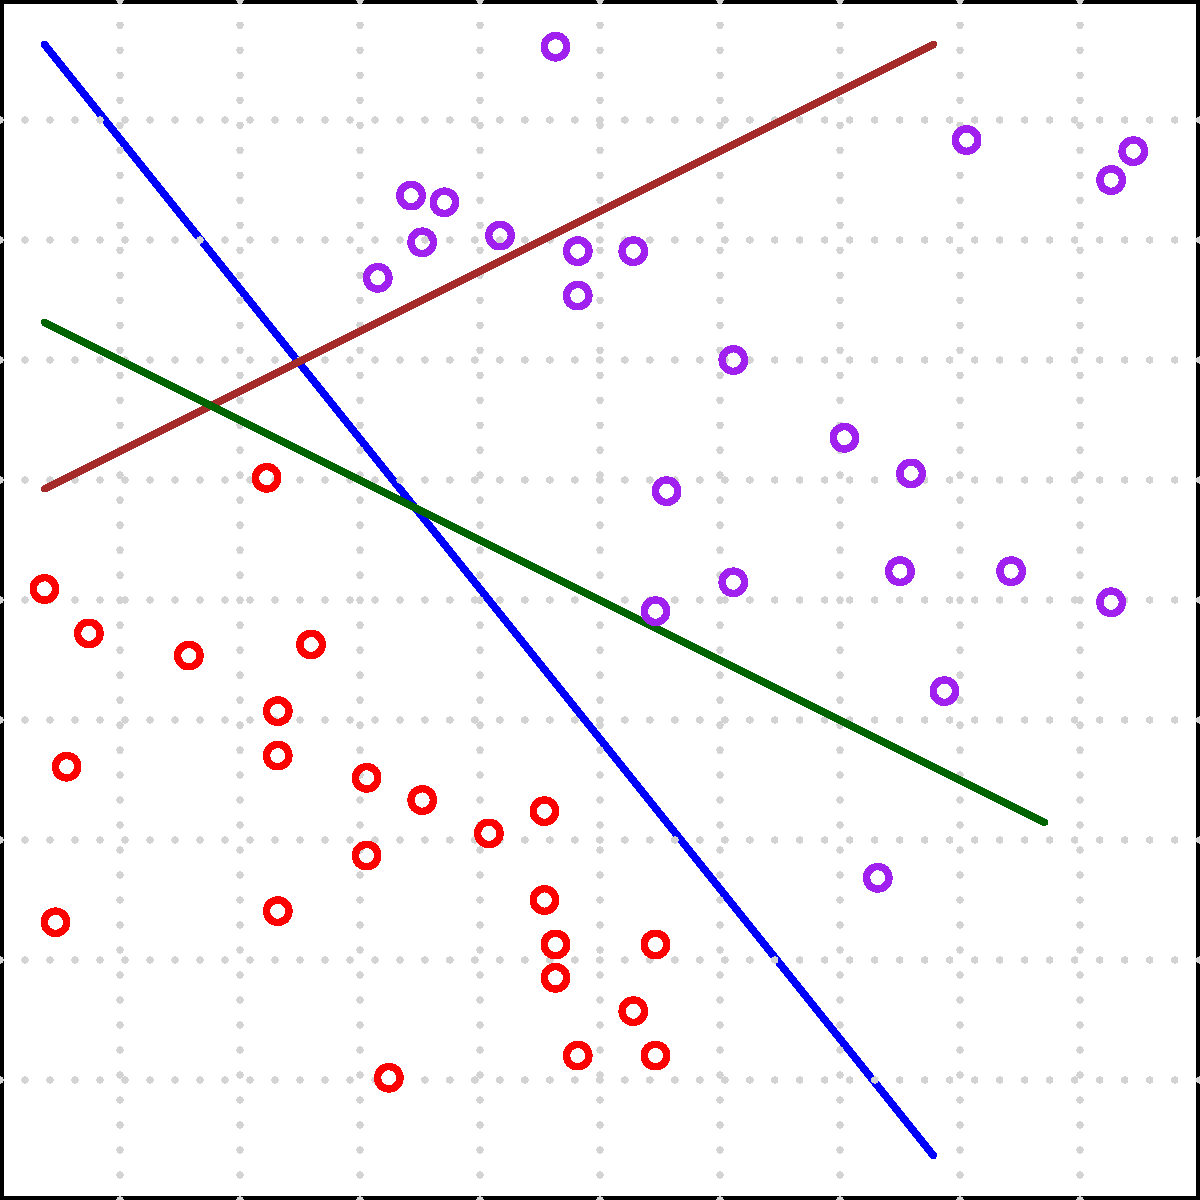
\includegraphics[width=0.60\columnwidth]{./plots/empirical_risk.pdf}
\caption[Empirical risk minimization.]{Empirical risk. Points in 2D space of two classes (red and purple) are classified by three linear classifiers (blue, green and dark red lines). The measure of success is to minimize empirical risk with respect to the number of misclassified points. The dark red lines leads five points to be misclassified, one point is misclassified by the green line, and the blue line has all points correctly classified. Therefore the blue line is the best separator in this case.}
\label{empirical_risk}
\end{center}
\end{figure}

Linear perceptron (e.g. \cite{freund99}) is an algorithm that is guaranteed to find a solution in a finite number of steps, with regards to minimizing empirical risk. However, the solution from linear perceptron algorithm is not unique when there exists more than one function to separate two classes of points that have the same empirical risk, shown in Figure~\ref{linear_perceptron}. The solutions are greatly affected by the initial values of $\wb$ and $b$, as well as the order to which observations in $\Scal$ are presented to perceptron. 

\begin{figure}[t]
\begin{center}
\centering
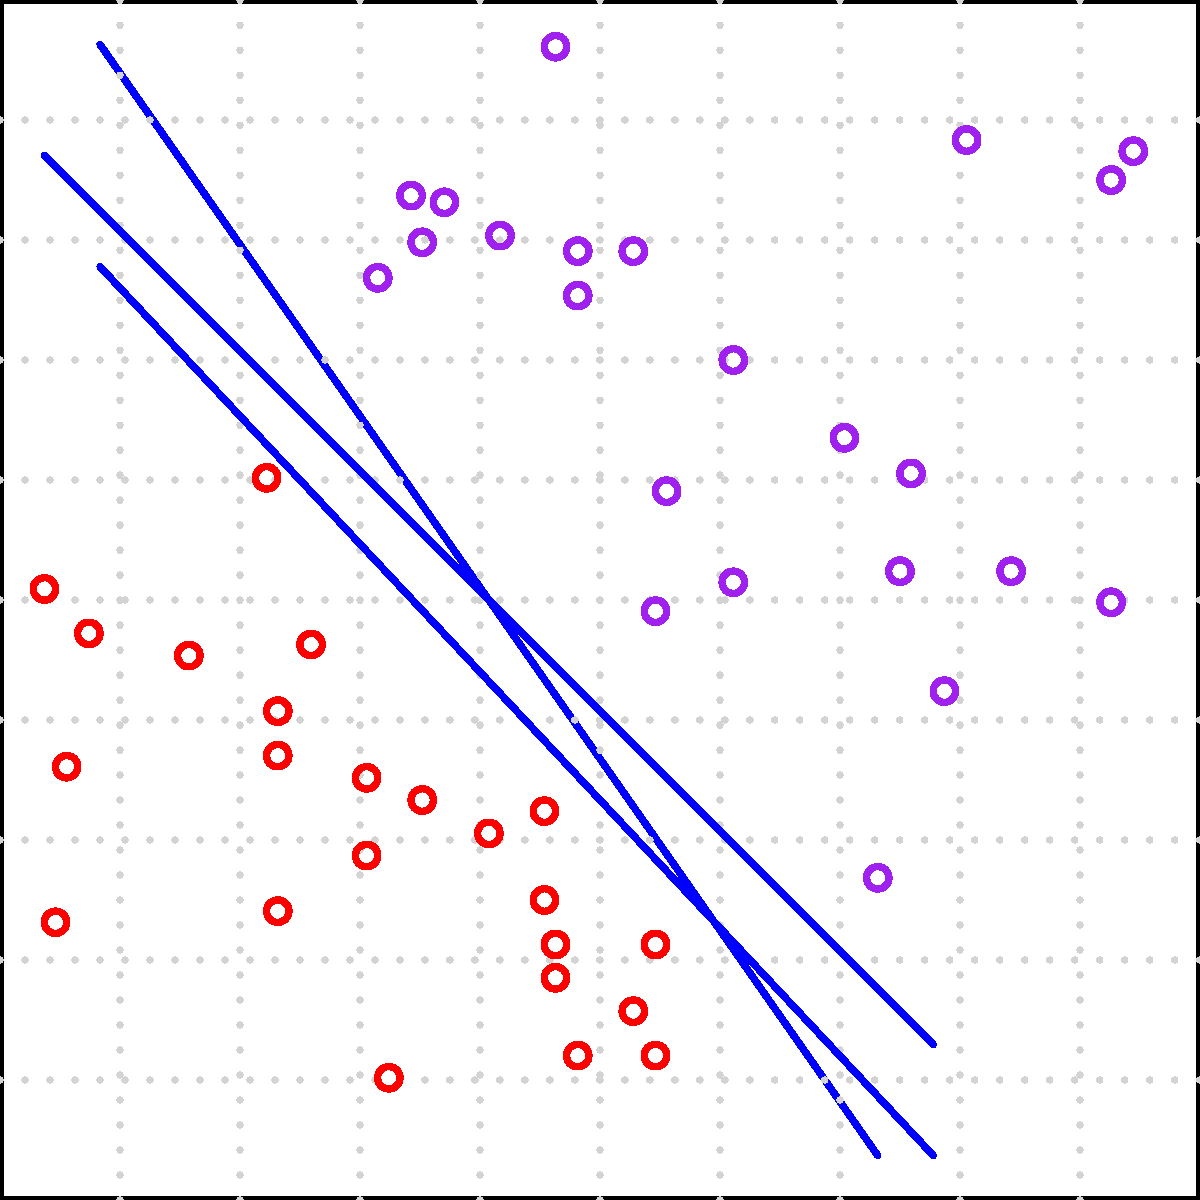
\includegraphics[width=0.60\columnwidth]{./plots/linear_perceptron.pdf}
\caption[Linear perceptron description.]{Linear perceptron. Points in 2D space are classified by three hyperplanes. Data are linearly separable and all of three hyperplane can correctly classify the data points. Therefore they are equivalent classifiers with respect to empirical risk minimization. The empirical risk principle does not uniquely define the solution in this case.}
\label{linear_perceptron}
\end{center}
\end{figure}

% hard margin

When multiple solutions exist, SVM employs the concept of {\em margin maximization} to work out this problem. {\em Margin} is defined as the distance between the decision boundary and the the closest data point. {Margin maximization} is to select a hyperplane with largest distances towards the closest data points, shown in Figure~\ref{margin_maximization}. Margin maximization can lead to a good generalization that has small error on unseen data points.

\begin{figure}[t]
\begin{center}
\centering
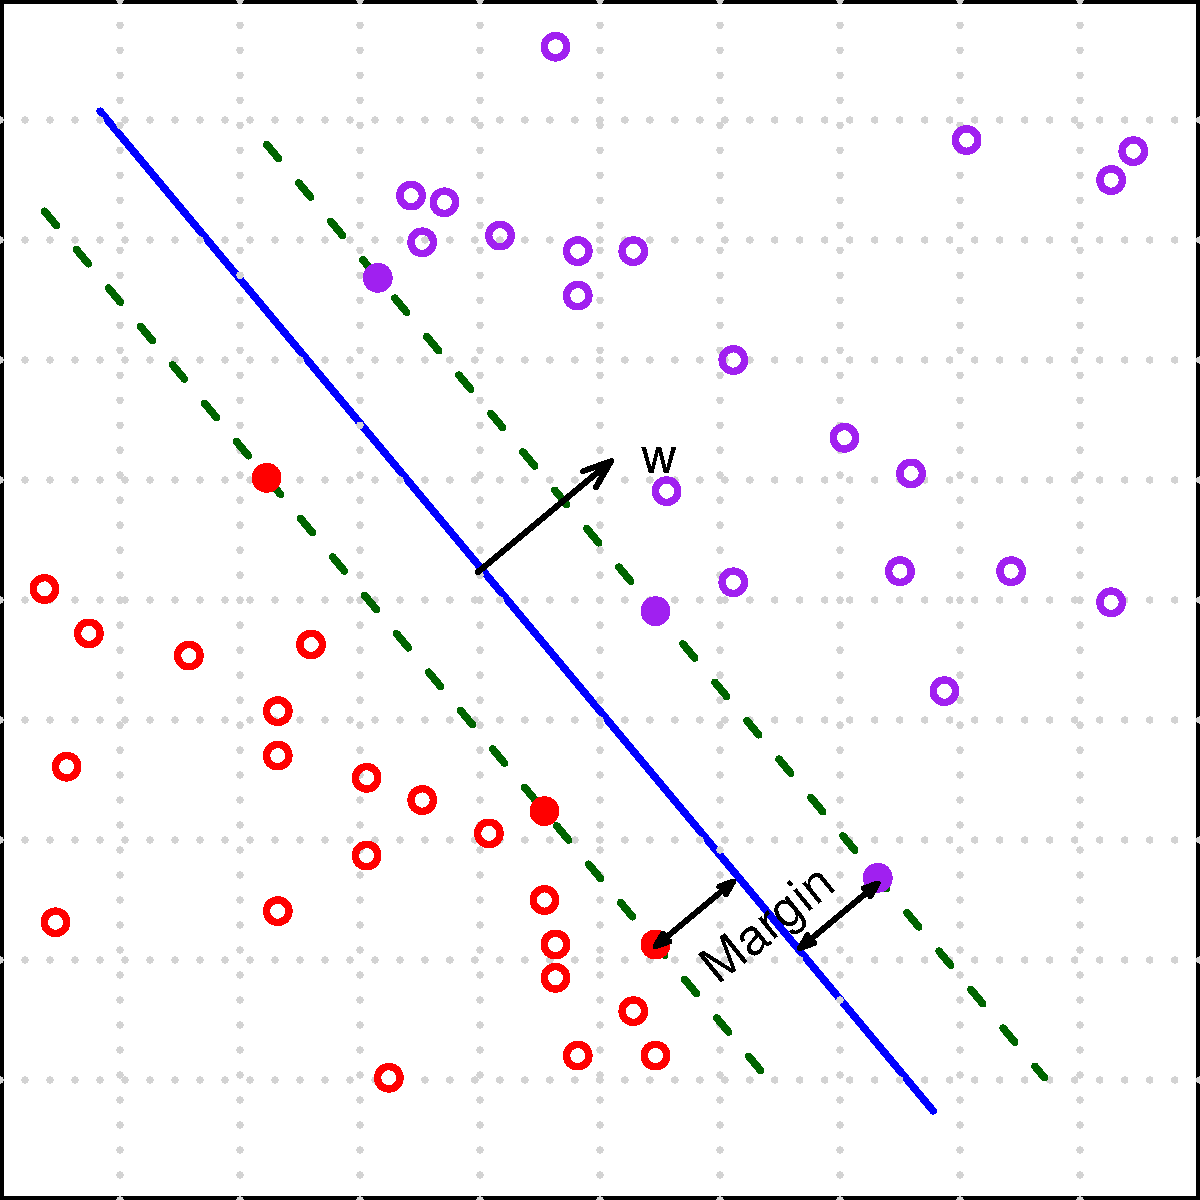
\includegraphics[width=0.60\columnwidth]{./plots/margin_maximization.pdf}
\caption[Margin maximization.]{Margin maximization. Data are linearly separable. A hyperplane defined by parameters $\wb$ and $b$ is shown as a blue line. The distance between the closest data points and the blue line is defined as margin. The green dashed lines are margin hyperplanes. Data points on margin hyperplanes are the so called support vectors.}
\label{margin_maximization}
\end{center}
\end{figure}

% hard margin optimization

Assume data are linearly separable in training data set $\Scal$. We can always select a hyperplane for each of two classes and make sure there are no data points between them. Decision boundary locates in the middle of the two hyperplanes. We try to maximize the distance between the two hyperplanes which also maximizes the distance between the decision boundary and the closest data points, the {margin} of SVM. The distance between two hyperplane is found to be $\frac{2}{||\wb||}$. Hence, {margin maximization} is to minimize $||\wb||$ with the constraint that each data point is correctly classified. This is commonly known as {\em hard margin SVM} and can be defined as the following optimization problem
\begin{align}
(\wb,b) & = \underset{\wb,b}{\operatorname{\argmin}} \, \frac{1}{2} ||\wb||^2,
\label{hard_margin_def} \\
\text{ s.t. } & y_i\,(\wb^T\xb_i + b) \ge 1,
\label{hard_margin_constraint} \\
 & 1 \leq i \leq n. \nonumber
\end{align}

% primal

This is an example of {\em quadratic programming} problem, which is to minimize a quadratic function with constraints of a set of linear equalities. SVM is not directly solved by (\ref{hard_margin_def}), but by {\em dual optimization}. We introduce a set of {\em Lagrange multipliers} $\valpha = (\alpha_i,\cdots,\alpha_n)$ with $\alpha_i \ge 0$ for all $i$, one for each constraint of (\ref{hard_margin_constraint}). It results in the {\em primal representation} of Lagrange function, where we minimize
\begin{align}
\Lcal(\wb, b, \valpha) = \frac{1}{2}||\wb||^2 - \sum_{i = 1}^n{\alpha_i(y_i(\wb^T \xb_i + b)-1)}.
\label{hard_margin_primal}
\end{align}
The Lagrange function can be interpreted as minimization with respect to $\wb$ and $b$ and maximization with respect to $\alpha_i$. Taking the partial derivatives of $\Lcal(\wb, b, \valpha)$ with respect to $\wb$ and $b$ results in following two constraints:
\begin{align*}
\frac{\partial \Lcal}{\partial \wb} &=  \wb - \sum_{i = 1}^{n}{\alpha_i y_i \xb_i} = 0, \\
\frac{\partial \Lcal}{\partial b} &=  \sum_{i = 1}^{n}{\alpha_i y_i} = 0.
\end{align*}

% dual form

Inserting the constraints from partial derivatives back to the primal (\ref{hard_margin_primal}) gives the {\em dual representation}, in which we maximize
\begin{align}
\tilde{\Lcal}(\valpha) = \sum_{i=1}^{n}{\alpha_i} - \sum_{i = 1}^{n}\sum_{j = 1}^{n}{\alpha_i \alpha_j y_i y_j (\xb_i \cdot \xb_j)},
\label{hard_margin_dual}
\end{align}
where $(\xb_i\cdot \xb_j)$ denotes the inner product of observations $\xb_i$ and $\xb_j$. It is subject to the positivity constraint $\alpha_i \ge 0$ for $1 \leq i \leq n$ and the equality constraint $\sum_{i=1}^{n}{\alpha_i y_i} = 0$.

% classify new data points

Predictions can be made by evaluating the sign of (\ref{svm_def}). Using learned parameters $\valpha$ to substitute $\wb$ results in
\begin{align}
f(\xb) = \sum_{i = 1}^{n}{\alpha_i y_i (\xb_i \cdot \xb)} + \bb.
\label{hard_margin_decision}
\end{align}

% support vectors

According to Karush-Kuhn Tucker (KKT) conditions \cite{kuhn50}, among observations $(\xb_i, y_i)$ in training data set $\Scal$, ones that lies on the correct side of the margin hyperplane will have $\alpha_i = 0$. They play no role in making predications of new data points, seen from (\ref{hard_margin_decision}). The remaining observations will have $\alpha_i > 0$. They locate on the margin hyperplane and satisfy $y_if(\xb_i) = 1$. These observations are known as {\em support vectors}, and are important in SVM theory. After one learns a model from training data set, only a small proportion of examples need to be retained while others can be discarded.

% calculate b

Once we solve the quadratic problem and find the values of $\valpha$, we can determine the parameter $b$ by using the equality $y_if(\xb_i) = 1$ of any support vector $(\xb_i, y_i)$. Combining with (\ref{hard_margin_decision}) leads to
\begin{align}
y_j\left(\sum_{i = 1}^{n}{\alpha_i y_i (\xb_i \cdot \xb_j)} + b\right) = 1.
\label{hard_margin_b_1}
\end{align}
Since non-{\em support vectors} will have $\alpha_i = 0$, we further rewrite the (\ref{hard_margin_b_1}) with only {\em support vectors} as:
\begin{align}
y_j\left(\sum_{m \in \SVcal}{\alpha_m y_m (\xb_m \cdot \xb_j)} + b\right) = 1,
\label{hard_margin_b_2}
\end{align}
where $\SVcal$ denote the index set of support vectors. Therefore, we can obtain the value of parameter $b$ with an arbitrary support vector by:
\begin{align*}
b = y_i - \sum_{m \in \SVcal}{\alpha_m y_m (\xb_m \cdot \xb_i)}
\end{align*}
For numerical stability \cite{higham96}, one common way is to take the average value of $b$ obtained from each support vector by:
\begin{align*}
b = \frac{1}{\Ncal_{\SVcal}}\sum_{i \in \SVcal}{\left(y_i - \sum_{m \in \SVcal}{\alpha_m y_m (\xb_m \cdot \xb_i)}\right)},
\end{align*}
where $\Ncal_{\SVcal}$ is the total number of support vectors.


\subsection{Soft margin optimization}

% slack parameter 

So far we have assumed that training data are linearly separable and hard margin SVM can exactly classify examples in two classes. In most real world cases data are not linearly separable. Training examples of two classes in feature space $\Xcal$ may overlap with each other. It is sometimes possible to classify all examples with a non-linear separator. However, this may lead to loss of generality and poor predictions of unseen data points.

We need to modify hard margin SVM to allow some of training examples be misclassified, shown in Figure~\ref{soft_margin}. We therefore introduce $n$ new parameters $\xi = (\xi_1,\cdots,\xi_n)$ where $\xi_i \ge 0$, with one for each training data points. Parameters $\xi$ are known as {\em slack parameters}, and were first introduced in \cite{cortes95}. They are defined so that $\xi_i = 0$ corresponds to data points that are outside or on the margin boundary, and $\xi_i = |y_i - f(\xb_i)|$ for others. More specifically, data points with $0<\xi_i<1$ locate between margin boundary and decision boundary, ones with $\xi_i = 1$ are on decision boundary, and ones with $\xi_i>1$ are misclassified.

\begin{figure}[t]
\begin{center}
\centering
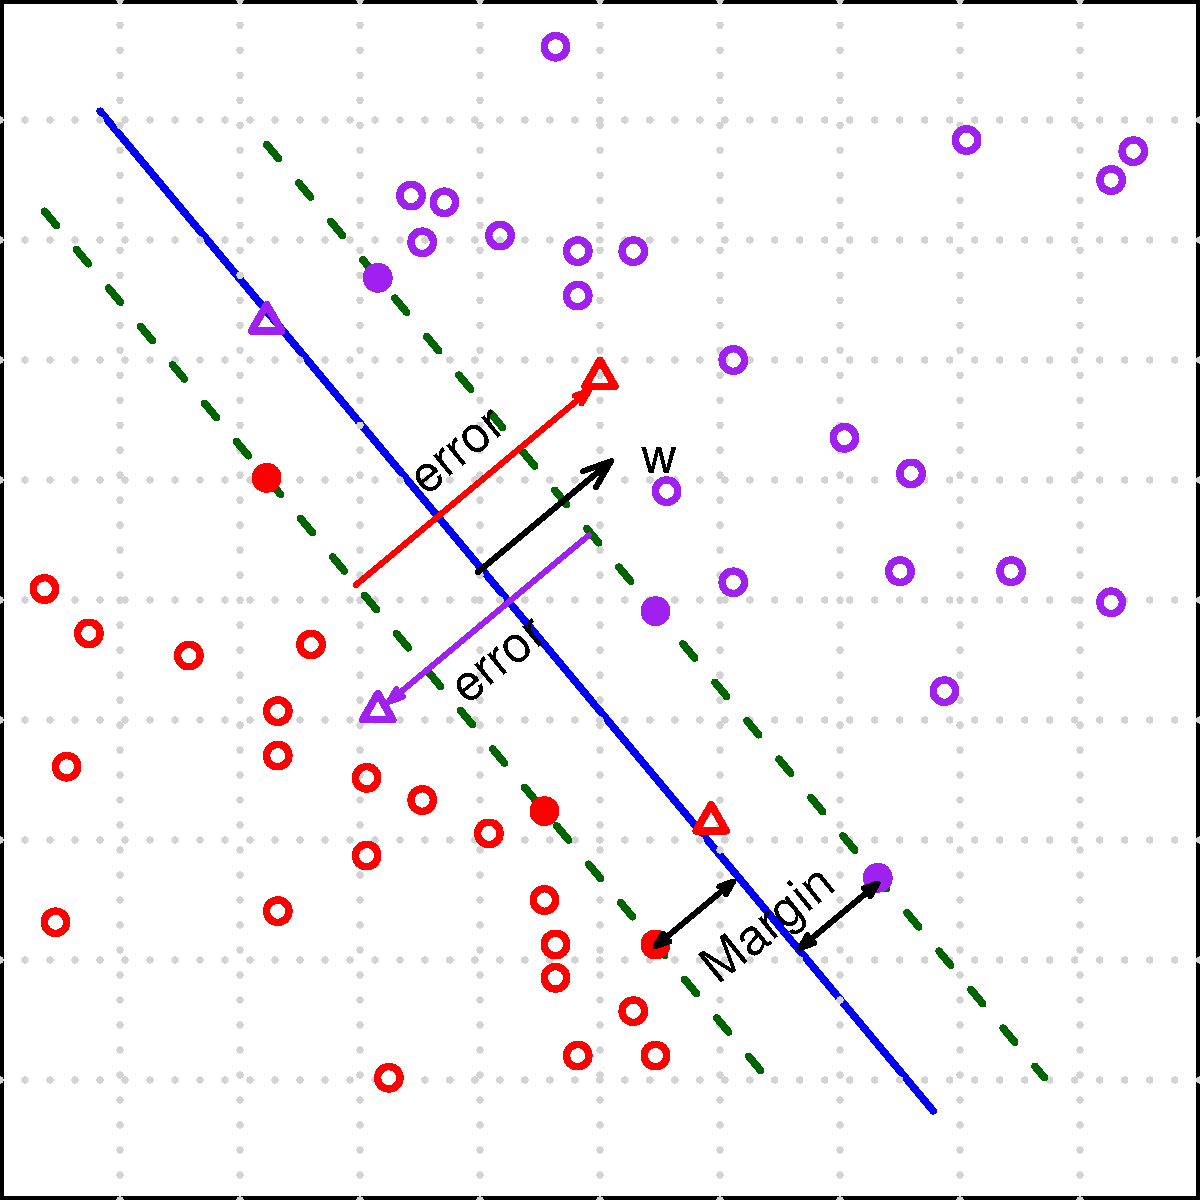
\includegraphics[width=0.60\columnwidth]{./plots/soft_margin.pdf}
\caption[Soft margin SVM.]{Soft margin SVM. The majority of data are linearly separable (circle points), with some of them overlaps (triangle points). A hyperplane is shown to classify points into two classes with respect to maximizing the margin. The optimization of soft margin SVM allows some points to be misclassified at the same time.}
\label{soft_margin}
\end{center}
\end{figure}

% soft margin and soft margin SVM

Intuitively, hard margin constraint being relaxed by slack parameters leads to a {\em soft margin}. The goal is therefore to maximize margin while penalize the data points that locate on the wrong side of margin boundary. This is commonly known as {\em soft margin SVM} and can be defined as the following optimization problem:
\begin{align}
(\wb,b)  &= \underset{\wb,b}{\operatorname{\argmin}}\left( \frac{1}{2} ||\wb||^2 + C \sum_{i=1}^m \xi_i \right) \text{,} \label{soft_margin_def} \\
\text{ s.t. } & y_i\,(\wb^T \xb_i + b) \ge 1 - \xi_i \text{,} \label{soft_margin_constraint_1} \\
 & \xi_i \ge 0  \text{, } 1 \leq i \leq n \text{,} \label{soft_margin_constraint_2} 
\end{align}
where $C > 0$ is the parameter that balances the margin maximization and penalties of misclassified examples (training errors). When $C \to \infty$, misclassifications are weighted so greatly that soft margin SVM defined in (\ref{soft_margin_def}) goes back to the earlier hard margin SVM defined in (\ref{hard_margin_def}).

% soft margin optimization

% primal

This is also an example of quadratic programming problem. We process the problem with Lagrange multiplier by introducing $\valpha = (\alpha_i,\cdots,\alpha_n)$ with one for each constraint of (\ref{soft_margin_constraint_1}), and $\vbeta = (\beta_i,\cdots,\beta_n)$ with one for each constraint of (\ref{soft_margin_constraint_2}). It leads to primal form of Lagrange function, where we minimize
\begin{align}
\Lcal(\wb, b, \xib, \valpha, \vbeta) = \frac{1}{2}||\wb||^2  + C\sum_{i=1}^{n}{\xi_i}- \sum_{i = 1}^n{\alpha_i(y_i(\wb^T \xb_i + b)-1 + \xi_i) - \sum_{i=1}^{n}{\beta_i \xi_i}} \text{.}
\label{soft_margin_primal}
\end{align}
Taking the partial derivatives of $\Lcal(\wb, b, \xib, \valpha, \vbeta)$ with respect to $\wb$, $b$ and $\xib$ results in following constraints:
\begin{align*}
\frac{\partial \Lcal}{\partial \wb} &=  \wb - \sum_{i = 1}^{n}{\alpha_i y_i \xb_i} = 0 \text{,} \\
\frac{\partial \Lcal}{\partial b} &=  \sum_{i = 1}^{n}{\alpha_i y_i} = 0 \text{,} \\
\frac{\partial \Lcal}{\partial \xi_i} &=  C - \alpha_i - \beta_i = 0 \text{, } 1 \leq i \leq n \text{.}\
\end{align*}

% dual form

Plunging the constraints from partial derivatives back to primal defined in (\ref{soft_margin_primal}) and eliminating $\wb$ and $b$ gives the dual form, in which we maximize
\begin{align}
\tilde{\Lcal}(\valpha) = \sum_{i=1}^{n}{\alpha_i} - \sum_{i = 1}^{n}\sum_{j = 1}^{n}{\alpha_i \alpha_j y_i y_j (\xb_i \cdot \xb_j)} \text{,}
\label{soft_margin_dual}
\end{align}
\begin{align*}
\text{ s.t. } & 0 \leq \alpha_i \leq C \text{,} 1 \leq i \leq n \text{,}\\
 & \sum_{i = 1}^{n}{\alpha_i y_i} = 0 \text{.}
\end{align*}
This is almost identical to the dual form of hard margin SVM defined in (\ref{hard_margin_dual}), except subjecting to different constraints. Once $\alpha_i$ is obtained, another dual variable $\beta$ can be found as:
\begin{align*}
\beta_i = C-\alpha_i \text{, }  1 \leq i \leq n \text{.}
\end{align*}

% decision, support vectors, calculating b

Similarly, predictions for new data points are based on (\ref{hard_margin_decision}). Training examples with $\alpha_i = 0$ do not affect the decisions. Examples with $\alpha_i = C$ require $\beta_i = 0$ which leads to either $\xi_i = 0$ corresponding to being inside the margin, or $0<\xi_i<1$ corresponding to being between margin boundary and decision boundary, or $\xi_i \ge 1$ corresponding to being misclassified. According to KKT condition, examples with $0<\alpha_i<C$ result in $\xi_i =0$, which correspond to being exactly on the margin boundary. They are support vectors in soft margin SVM. A numeric stable solution for $\bb$ is given by
\begin{align*}
b = \frac{1}{\Ncal_{\SVcal^{'}}}\sum_{i \in \SVcal^{'}}{\left(y_i - \sum_{m \in \SVcal^{'}}{\alpha_m y_m (\xb_m \cdot \xb_i)}\right)},
\end{align*}
where $\Ncal_{\SVcal^{'}}$ is the total number of support vectors in soft margin SVM that have $0<\alpha_i<C$.


\subsection{Non-linear SVM}

% introduction to non-linear svm

In the previous cases, we have discussed the SVM algorithm in the scope that an optimal classification hyperplane exists for a linear separation of training data. However, the optimal separation surface are not simply linear in many cases. Even with slack parameters, it is not possible to separate the training data with a linear separator, as shown in Figure~\ref{nonlinear_svm}. 

\begin{figure}[t]
\begin{center}
\centering
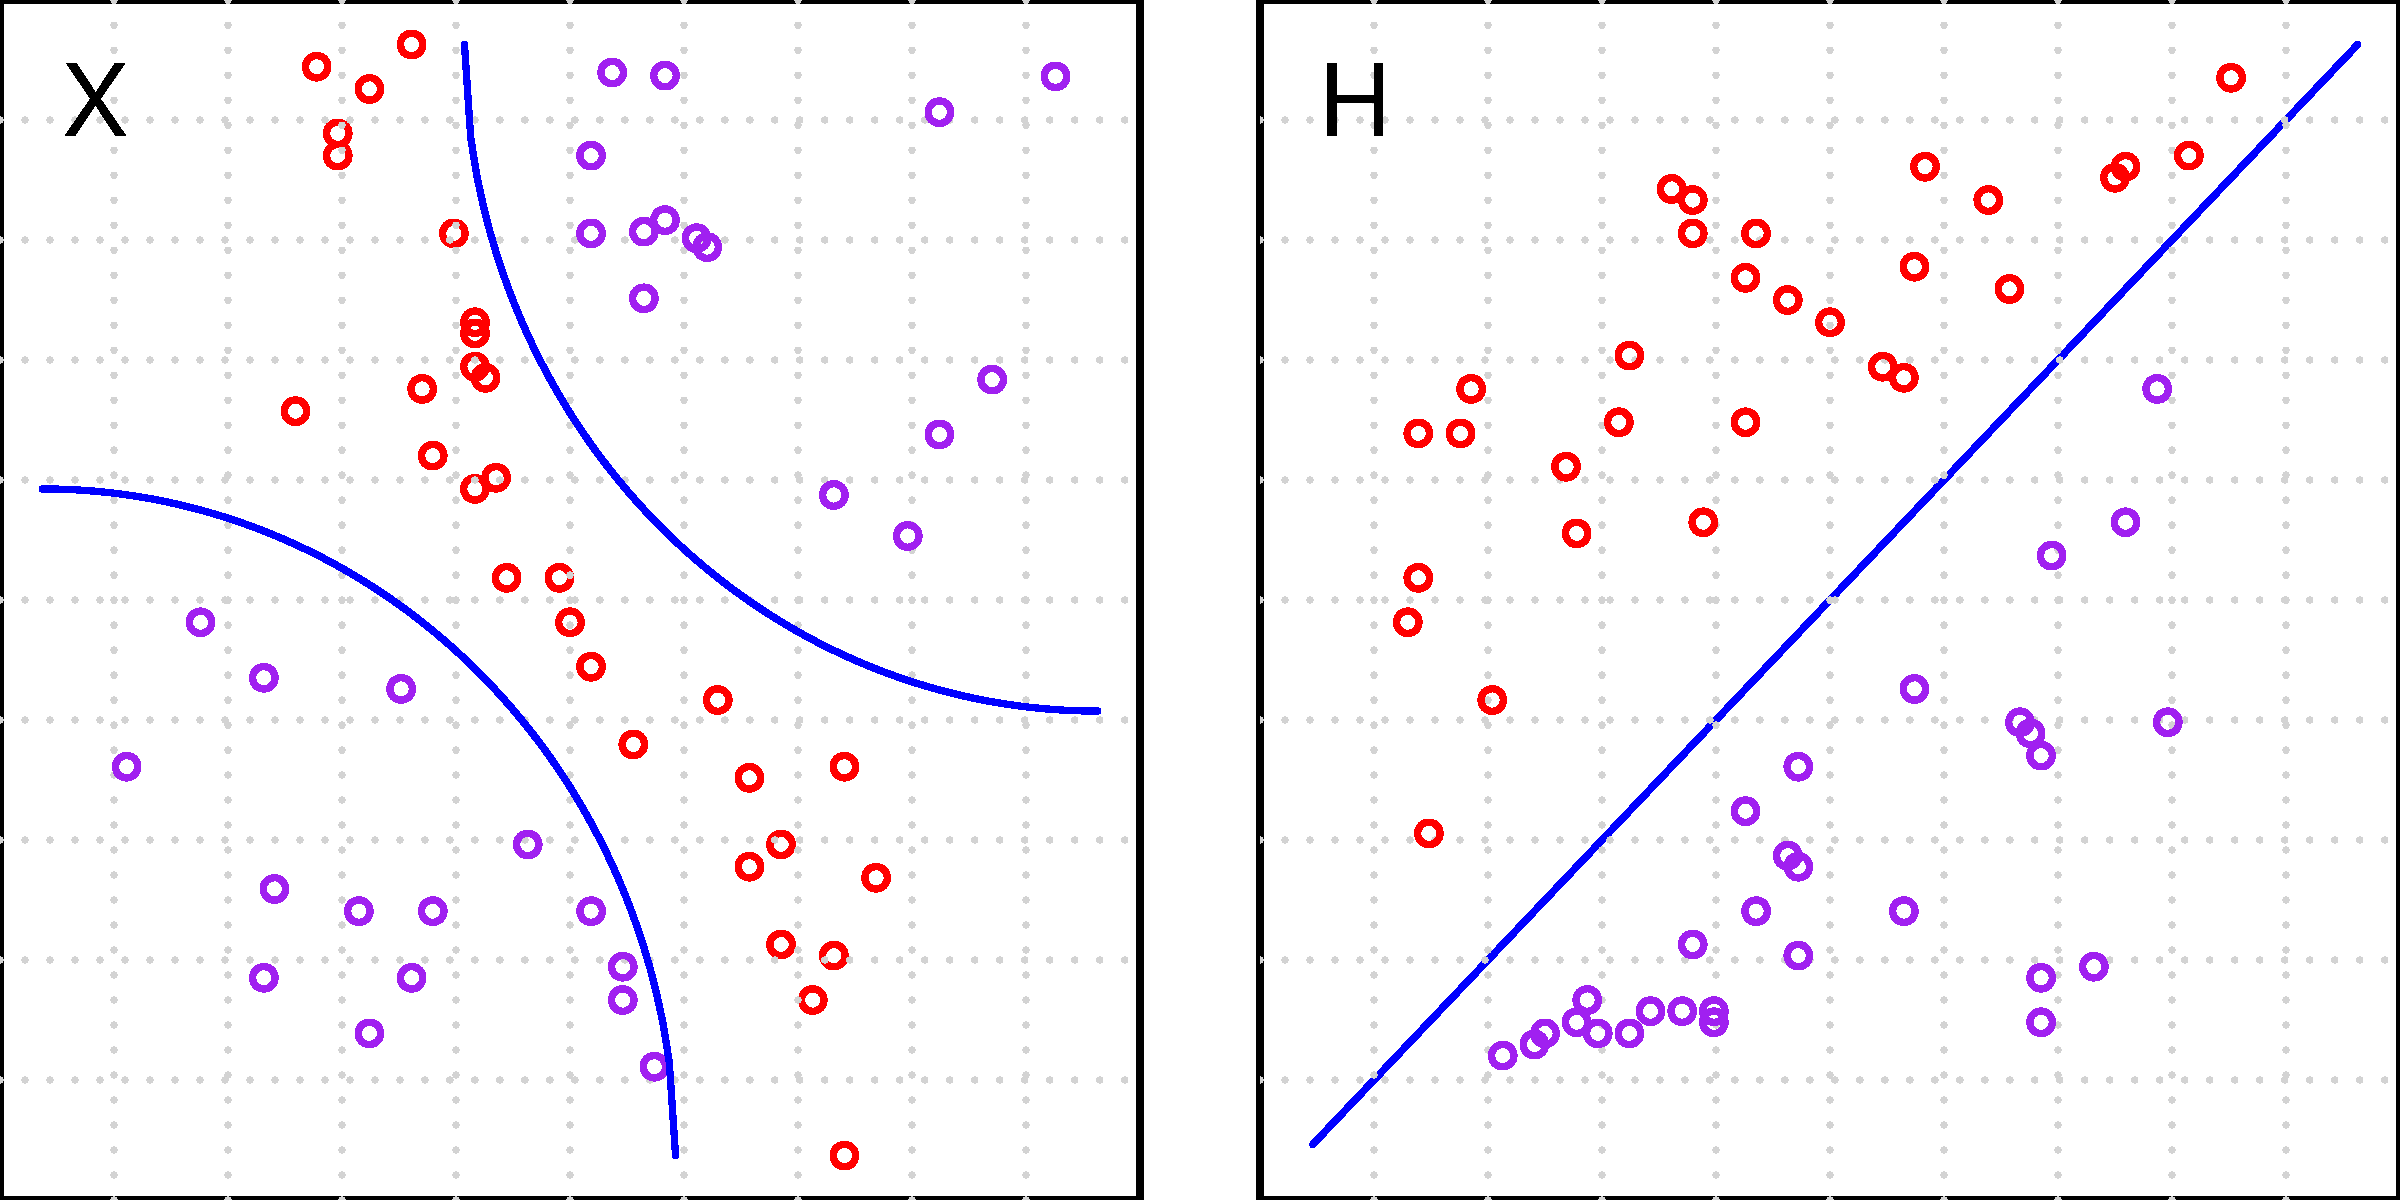
\includegraphics[width=.9\columnwidth]{./plots/kernel_svm.pdf}
\caption[Non-linear SVM.]{Non-linear SVM. Left, data points in 2D space are given in two classes. Even using soft-margin SVM with slack parameter $\xib$, it is not possible to classify the data points with a linear hyperplane. Right, non-linear SVM uses a feature mapping function $\varphi$ to transform data points in input space to a high dimensional feature space $\Hcal$. There may exist a linear separator in $\Hcal$ that can classify the data points.}
\label{nonlinear_svm}
\end{center}
\end{figure}

% feature mapping function

We can extend support vector machine to tackle the non-linear data by means of a feature mapping function $\varphi(\xb)$, which transforms the examples in input space $\Xcal$ to a higher dimensional feature space $\Hcal$, where training data is supposed to be classified by a linear separator. $\Hcal$ is commonly known as a {\em Hilbert} space with finite or infinite dimensions. Mathematically, training dataset \(\Scal\) consists of a series of $n$ objects \(\Xcal = \xb_1,\xb_2,\cdots,\xb_n \in \mathbb{R}^n\), where $\xb_i$ is a $n$ dimensional vector $\xb_i = (x_1, x_2,\cdots,x_n)$. A feature mapping function is comprised by a set of functions $\varphi = (\varphi_1, \varphi_2, \cdots, \varphi_k)$ that transfers each example $\xb_i$ to $\varphi(\xb_i)$, defined as
\begin{align*}
\xb_i = (x_1,x_2,\cdots,x_n) \xrightarrow{\varphi} \varphi(\xb_i) = (\varphi_1,\varphi_2,\cdots,\varphi_k) \text{.}
\end{align*}
Note $\xb_i$ and $\varphi$ can be in different dimensions, finite or infinite. As a result, we obtain a set of objects in high dimensional feature space $\varphi(\Xcal) = (\varphi(\xb_i), \varphi(\xb_2),\cdots,\varphi(\xb_n)) \in \Hcal$. Intuitively, even if training data in the input space $\Xcal$ are not linear separable, they may be separated by a hyperplane in high dimensional feature space $\Hcal$ if there exists an appropriate feature mapping function $\varphi:\xb \xrightarrow{\varphi} \varphi(\xb)$. The support vector machine with a non-linear feature mapping function is known as {\em non-linear SVM}, shown in Figure~\ref{nonlinear_svm}.

% formal definition of non-linear SVM

Substitute $\xb$ by $\varphi(\xb)$ in equations that defines the soft-margin SVM, we can obtain the mathematical formulations of the non-linear SVM. Specifically, optimization problem given in primal form is to minimize
\begin{align}
\Lcal(\wb, \bb, \xib, \valpha, \vbeta) = &\frac{1}{2}||\wb||^2  + C\sum_{i=1}^{n}{\xi_i}- \sum_{i = 1}^n{\alpha_i(y_i(\wb^T \varphi(\xb_i) + \bb)-1 + \xi_i) - \sum_{i=1}^{n}{\beta_i \xi_i}} \text{.}  \label{nonlinear_primal} 
%\text{ s.t. } &\frac{\partial \Lcal}{\partial \wb} =  \wb - \sum_{i = 1}^{n}{\alpha_i y_i \varphi(\xb_i)} = 0 \text{,} \nonumber \\
% &\frac{\partial \Lcal}{\partial \bb} =  \sum_{i = 1}^{n}{\alpha_i y_i} = 0 \text{,} \nonumber \\
% &\frac{\partial \Lcal}{\partial \xi_i} =  C - \alpha_i - \beta_i = 0 \text{, } 1 \leq i \leq n \text{.}\nonumber
\end{align}
The corresponding dual form is given by maximizing
\begin{align}
\tilde{\Lcal}(\valpha) = &\sum_{i=1}^{n}{\alpha_i} - \sum_{i = 1}^{n}\sum_{j = 1}^{n}{\alpha_i \alpha_j y_i y_j (\varphi(\xb_i) \cdot \varphi(\xb_j))} \text{.} \label{nonlinear_dual} 
%\text{ s.t. } & \sum_{i = 1}^{n}{\alpha_i y_i} = 0 \text{,} \nonumber \\
% & 0 \leq \alpha_i \leq C \text{,} 1 \leq i \leq n \text{.} \nonumber
\end{align}
Similarly, classification is done through the decision function give by
\begin{align}
f(\xb) = \sum_{i = 1}^{n}{\alpha_i y_i (\varphi(\xb_i) \cdot \varphi(\xb))} + \bb \text{.}
\label{nonlinear_decision}
\end{align}


\subsection{Kernel methods}
\label{kernel_sec}

% kernel comes out

Note that the problem of learning in non-linear separable data has been transformed to mapping data into feature space of higher dimension and performing a linear classification in the feature space. However, the dimensionality of feature space can be very high or even infinite and the feature mapping function can be quite complex. Therefore, we hope that we can avoid the direct inner product $\varphi(\xb_i) \cdot \varphi(\xb_j)$ in the feature space. This motivates the {\em kernel methods}. 

% TODO add definition
A function $K:\Xcal \times \Xcal \xrightarrow{K} \mathbb{R}$ is called {\em positive definite kernel} if and only if it is symmetric $K(\xb_i,\xb_j) = K(\xb_j,\xb_i)$ for any $\xb_i,\xb_j \in \Xcal$, and for any $C_i,C_j \ge 0$ it satisfies
\begin{align*}
\sum_{i=1}^{n}\sum_{i=1}^{n}{C_i C_j K(\xb_i, \xb_j)} \ge 0 \text{.}
\end{align*}
% TODO add theorem
It is also proved \cite{taylor04} that for any kernel function $K$ defined on the input space $\Xcal$, a mapping function $\varphi: \Xcal \xrightarrow{\varphi} \Hcal$ exists, which satisfies
\begin{align*}
K(\xb_i, \xb_j) = \varphi(\xb_i) \cdot \varphi(\xb_j) \text{, } \xb_i, \xb_j \in \Xcal \text{.}
\end{align*}
This property is very meaningful because we have to know neither the exact form of feature mapping function $\varphi$ nor the explicitly representations of objects in high dimensional feature space $\varphi(\xb)$. Only inner product is sufficient and can be calculated in input space with a kernel function.

Replacing inner product $\varphi(\xb_i) \cdot \varphi(\xb_j)$ with kernel function results in {\em kernel SVM}. The optimization problem in dual form is given by maximization of
\begin{align}
\tilde{\Lcal}(\valpha) = &\sum_{i=1}^{n}{\alpha_i} - \sum_{i = 1}^{n}\sum_{j = 1}^{n}{\alpha_i \alpha_j y_i y_j K(\xb_i, \xb_j)} \text{,} \label{kernel_dual} \\
\text{ s.t. } & \sum_{i = 1}^{n}{\alpha_i y_i} = 0 \text{,} \nonumber \\
 & 0 \leq \alpha_i \leq C \text{,} 1 \leq i \leq n \text{.} \nonumber
\end{align}
The decision function is given by
\begin{align}
f(\xb) = \sum_{i = 1}^{n}{\alpha_i y_i K(\xb_i, \xb)} + \bb \text{.}
\label{kernel_decision}
\end{align}

% kernel functions

Kernel function takes pairs of examples from input space. Therefore it can take various form, as long as it satisfies positive definite conditions. Commonly used kernel functions include:

{\em Linear Kernel} is the inner product of two training examples commonly used as a test for non-linear problem and serves as the reference for improvements achieved by other kernel functions, defined as
\begin{align*}
K(\xb_i,\xb_j) = (\xb_i \cdot \xb_j) \text{.}
\end{align*}
{\em Polynomial Kernel} is the simplest way to model the non-linear relationship which maps data into a higher dimensional space. The degree of the space is denoted by parameter $d$, and the parameter $c$ decides the smoothness of the resulted kernel. The polynomial kernel is defined as
\begin{align*}
K(\xb_i,\xb_j) = (\xb_i \cdot \xb_j + c)^d \text{.}
\end{align*}
{\em Radial Basis Function Kernel} is a widely used kernel function whose shape is controlled by parameter $\gamma$, defined as
\begin{align*}
K(\xb_i,\xb_j) = \exp(-\gamma{||\xb_i - \xb_j||^2}) \text{, } \gamma > 0 \text{.}
\end{align*}
{\em Gaussian Radial Basis Function Kernel} is another widely used kernel function which maps data into infinite dimension, defined as
\begin{align*}
K(\xb_i,\xb_j) = \exp(-\frac{||\xb_i - \xb_j||^2}{2\sigma}) \text{.}
\end{align*}
{\em Sigmoid Kernel} corresponds to the most used transformation function in neural networks with a sigmoid shape, defined as
\begin{align*}
K(\xb_i,\xb_j) = \tanh(a\xb_i \cdot \xb_j + b) \text{.}
\end{align*}
{\em Additive Kernel} follows one property of kernel function which is the summation of kernel functions is still a valid kernel function, defined as
\begin{align*}
K(\xb_i,\xb_j) = \sum_{m}{K_m(\xb_i,\xb_j)} \text{.}
\end{align*}
{\em Product Kernel} follows another property of kernel function which is the tensor product of kernel functions is still a valid kernel function, defined as
\begin{align*}
K(\xb_i,\xb_j) = \prod_{m}{K_m(\xb_i,\xb_j)} \text{.}
\end{align*}


Kernel normalization is independent of kernel types. It is defined as
\begin{align*}
\tilde{K}(\xb_i,\xb_j) = \frac{K(\xb_i,\xb_j)}{\sqrt{K(\xb_i,\xb_i)K(\xb_j,\xb_j)}} \text{.}
\end{align*}
This normalization ensures that the diagonal values of kernel matrix are $1$ and other values range from $0$ to $1$. It is quite important especially for generalized kernel functions, which are computed direct from objects other than feature representations. kernel normalization can avoid the biased results, for example bigger graph will result in large value in kernel matrix when calculating graph kernels.


\subsection{Multiclass SVM}

% multi class svm

The support vector machine is specially designed for classification of data in two classes, or so called binary classification problem. Many real world problem consists of, however, more than two classes. For example, functions of a protein or an enzyme can possibly belong to several EC families\footnote{http://www.brenda-enzymes.org/}. Therefore, several methods have been developed based on two-class SVM to tackle the multiclass problem.

% one method

One of the most popular way to solve the multiclass classification problem with $K$ classes is to split the problem into $K$ separate binary classification sub-problems \cite{vapnik98}. The $i'\text{th}$ sub-problem is defined such that only observations in the $i'\text{th}$ class are treated as positive examples, and other observations are treated as negative ones. For example, assume we have multiclass classification problem where the the label vector of training set is defined as
\begin{align*}
\Ycal = (4,4,1,1,3,3,2,2). \nonumber
\end{align*}
The four corresponding binary classification problem are defined as
\begin{align*}
\Ycal_1 = (-1,-1,-1,-1,-1,-1,+1,+1), \nonumber \\
\Ycal_2 = (+1,+1,-1,-1,-1,-1,-1,-1), \nonumber \\
\Ycal_3 = (-1,-1,-1,-1,+1,+1,-1,-1), \nonumber \\
\Ycal_4 = (-1,-1,+1,+1,-1,-1,-1,-1). \nonumber
\end{align*}
Once multiclass classification problem is divided, a two-class SVM is trained based on training data of each subproblem. This is known as {\em one-against-all} approaches. 

% problem

However, one-against-all approach has consistancy problems when an example is assigned positive target value by several binary classifiers at the same time, shown in the left of Figure~\ref{multiclass_svm}. The inconsistency can be roughly tackled by taking the class label with the maximum prediction value, defined by
\begin{align*}
(k) & = \underset{k \in K}{\operatorname{\argmax}} \, f_k(\xb).
\end{align*}
The label assignment schema is still problematic. Since each separate binary classifier is defined based on different optimization problem, the objective values may not be in the same range. There are still examples that cannot be assigned class labels.

% another problem

Another problem that comes with one-against-all strategy is that the labeling situation is quite biased in each binary classification sub-problem. Assume a multiclass classification problem with equivalent number of examples in five class. A binary classification sub-problem will have $20\%$ of training example be positive labeled and $80\%$ be negative labeled. Therefore, the balanced labeling distribution no more exists.

\begin{figure}[t]
\begin{center}
\centering
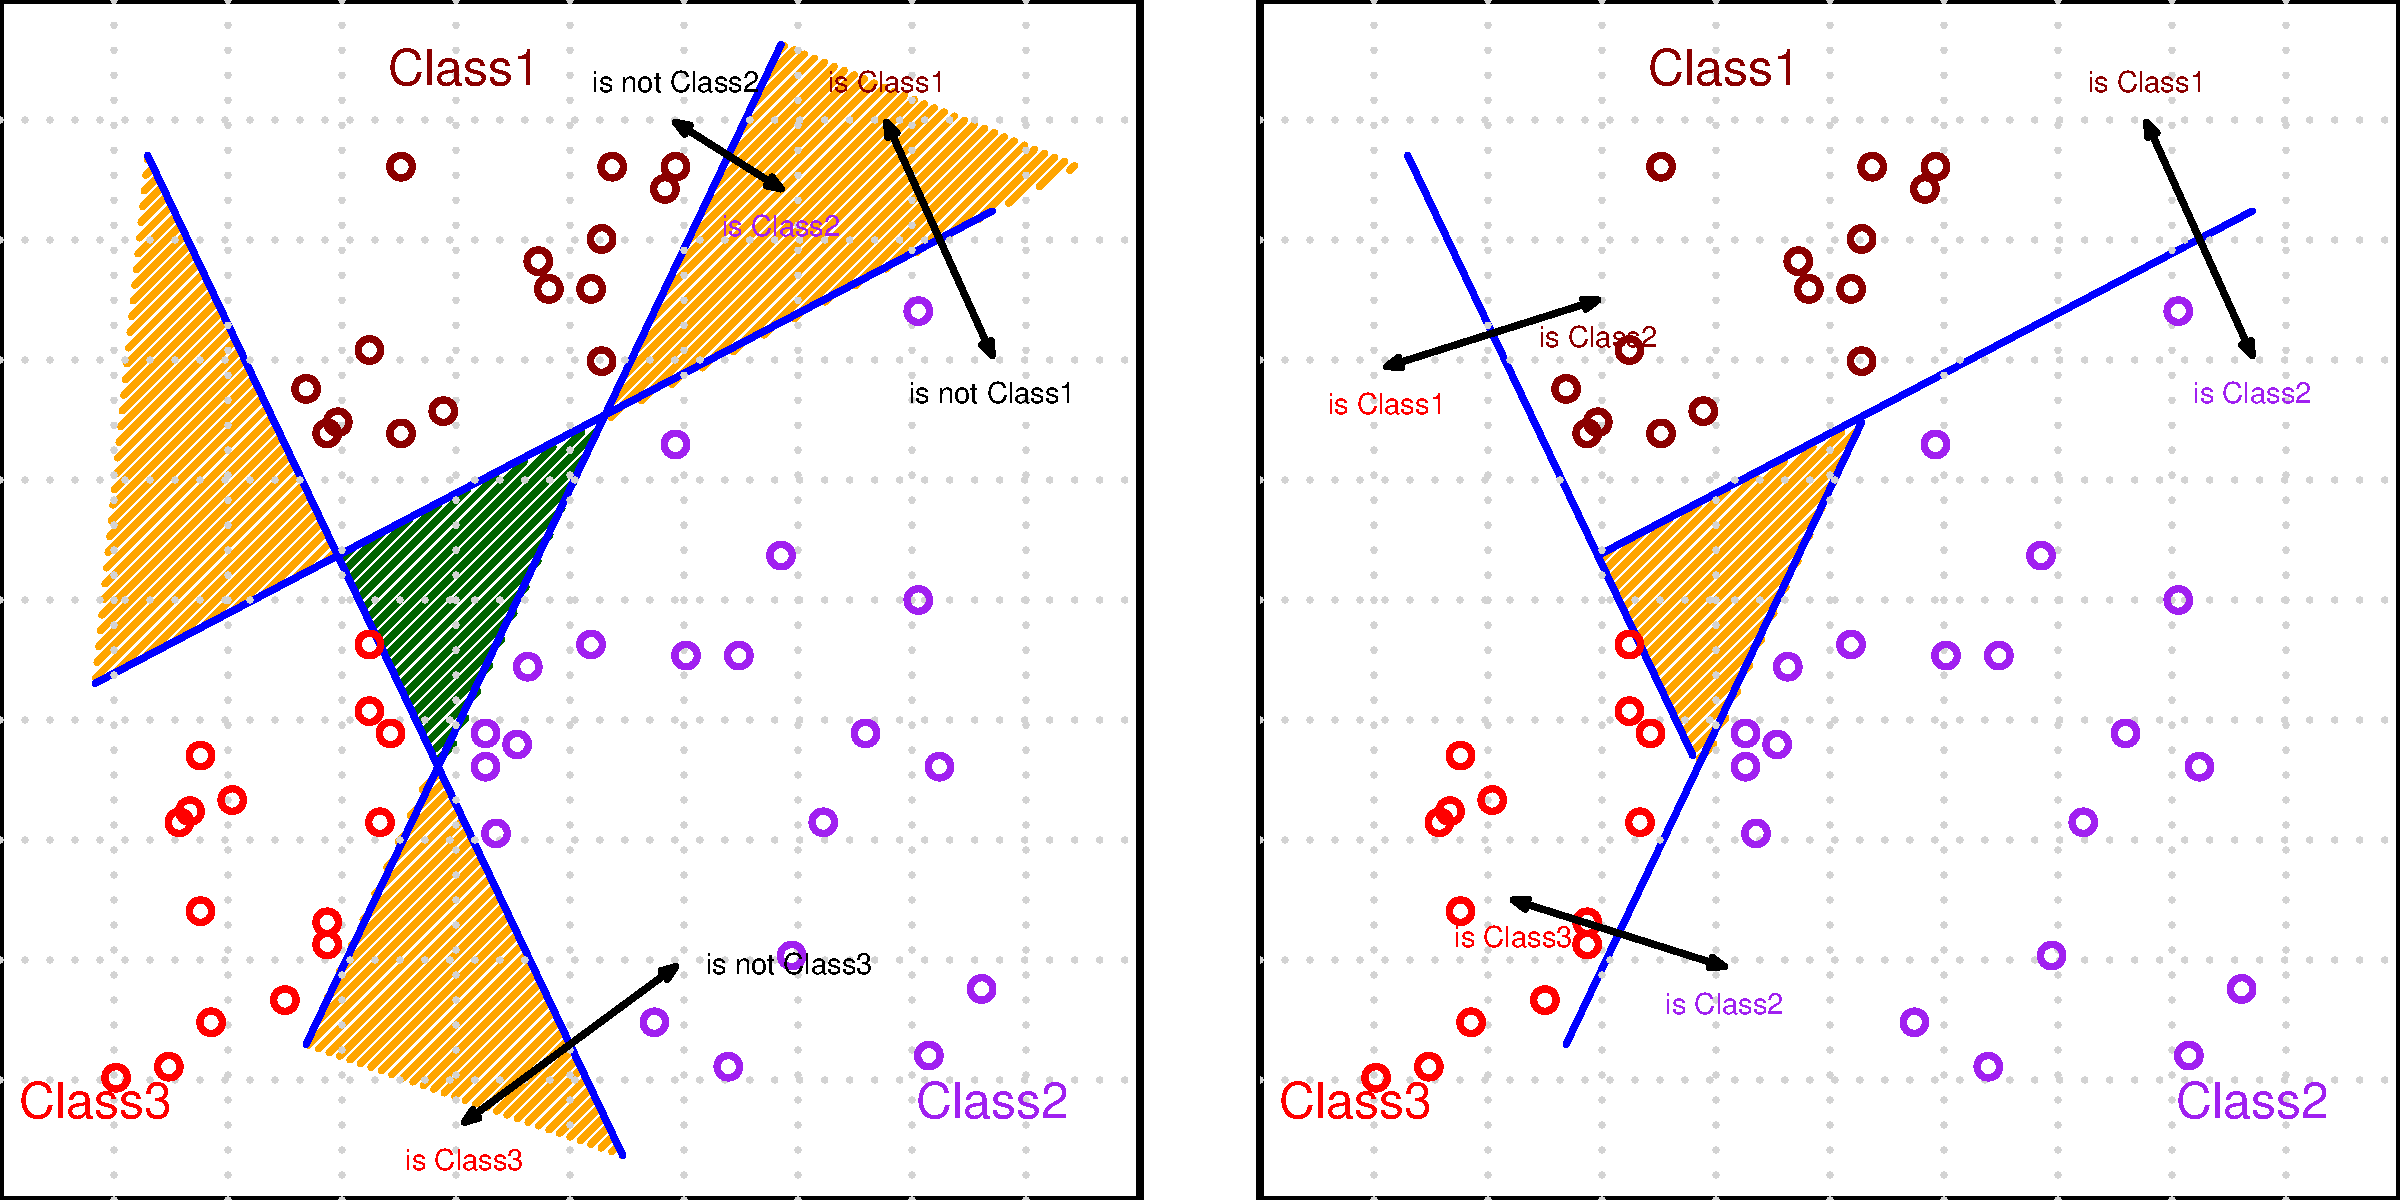
\includegraphics[width=.9\columnwidth]{./plots/multiclass_svm.pdf}
\caption[Multiclass support vector machines.]{Multiclass support vector machines. Left, points in three classes are separated by one-against-all approach. Inconstancy happens in the areas which belongs to more than one classes, as shown in orange areas. Blue area corresponding to the area resulted by crossing-over of three hyperplanes and therefore belongs to none of the three classes. Right, the inconstancy is addressed by one-again-one approach. Blue area does not exist in this approach. Inconstancy areas become smaller, while still exists.}
\label{multiclass_svm}
\end{center}
\end{figure}

% another approaches

A more elegant way for multiclass classification is to define the single objective function that considers all $K$ classifiers at the same time \cite{weston99}. The algorithm includes maximizing margin between pair of classes and remaining the number of classes. However, it needs more time to train such a classifier compared to one-against-all approach. 

Another method for multiclass classification is so-called {\em one-against-one} approach which aims to train $\frac{K(K-1)}{2}$ classifiers between any possible pair of classes \cite{kressel99}. The method assigns a label to an example following a majority vote stager. However, it still suffers from consistancy problem as one-against-all approach when one example is assigned several labels at the same time, shown in right of Figure~\ref{multiclass_svm}. 

Furthermore, there is a method for multiclass classification known as {\em error-correcting output code} \cite{allwein00}. It can be seen as generalized one-against-one approach. The method trains several binary classifiers, each of which takes several classes as positive class and the complementary classes as negative one. By using a smart way to partition the original classes and combining several binary classifiers, the method can alleviate the inconstancy inherited by multiclass classification problem. It is good alternative to most commonly used multiclass algorithms. 




\subsection{Multilabel classification}

%\subsubsection{Multilabel classification in general}

Compared to single label classification which assigns the object to one class when there exist two or more classes (corresponding to binary or multiclass classification), the multilabel classification is to categorize the object simultaneously to several classes \cite{ghamrawi05}. In the last ten years, multilabel classification has become increasingly important in many real world applications, for example music categorization \cite{juan03}, gene and enzyme function annotation \cite{barutcuoglu06, astikainen08}, image and document classification \cite{ghamrawi05}, medical diagnosis \cite{huang10} and molecular classification. 

A variety of models have been introduced for multilabel classification task, including approaches that use a collection of binary classifiers \cite{ghamrawi05, juan03, xiao07}. Other methods use Bayesian framework to combine multiple classifiers based on functional constraints \cite{barutcuoglu06, huang10}. These methods are usually referred as flat classification approach \cite{silla10}. However, objects are usually associated with hundred or thousand of labels. Most of the flat classification models do not scale well to such high computational demonds, as they are supposed to learn an individual classier for each possible label. Besides, the dependencies between labels are not explicitly modeled. Multilabels are mostly assumed to be independent in flat classification approaches.

Hierarchical classification emerged in recent years as an elegant way for multilabel classification task \cite{silla10}. It assumes an hierarchy exists over multilabels, and models the dependencies inside the hierarchy. Especially, hierarchical classification models combined with kernel methods help us manipulate high dimensional feature space without explicitly constructing feature maps. These methods include structured SVM \cite{THJA04}, M$^3$N \cite{taskar03}, HM$^3$ \cite{rousu2006kbl,rousu2007}, output kernel tree \cite{wehenkel06}, and max-margin regression \cite{szedmak06}. 


\subsubsection{Max-margin conditional random field (MMCRF)}

Max-margin conditional random field (MMCRF) is the method used in this thesis. It is an application of the algorithm developed in \cite{rousu2007}. In addition to original algorithm \cite{rousu2006kbl}, which was restricted to hierarchical tree structure, \cite{rousu2007} expands it for general graph structures. The model takes as inputs a Markov network over all labels and the kernel representation of the objects. It uses max-margin optimization for parameter learnings. Belief propagation inference is employed for learning parameters and constructing the predictions.

Mathematically, we assume that training data is comprised by a series of $n$ objects $\Xcal = x_1, x_2,\cdots,x_n$ and a set of labeling vectors $\Ycal = \Ycal_1 \times \Ycal_2 \times \cdots \times \Ycal_k$ which is a Cartesian product of the sets $\Ycal_j = \{-1,+1\}$ for $j = 1,\ldots, k$. There exists a labeling vector $\yb_i = (y_1,y_2,\cdots,y_k) \in \Ycal$, known as {\em multilabel}, associated to each object $x_i$. Each component of multilabel vector $\yb_i$ is called a {\em microlabel}, as denoted by $y_j$ for $j=1,\ldots,k$. The object and multilabel pair $(x_i,\yb_i) \in \Xcal \times \Ycal$ serving as training example is drawn from an unknown joint distribution $P(\Xcal, \Ycal)$. In addition, a pair $(x_i, \yb)$ where $\yb$ is an random labeling vector for object $x_i$ is called {\em pseudo example}. Training example and pseudo example are not necessarily from the same distribution. The task is to learn a conditional probability $P(\yb'|x')$, from where one can infer the most probable labeling vector $\yb'$ given an unknown object $x'$.

As mentioned previously, we have a Markov network $G = (\Vcal,\Ecal)$ defined over all labels, where node $v_j$ corresponds to the $j$th component of multilabel vector $\Ycal$, and edge $e = (v_j,v_i) \in \Ecal$ denotes the dependency relation between nodes $v_i$ and $v_j$. The conditional probability $P(\yb|x)$ can be modeled in factorization form of the exponential family based on the Markov network, defined as
\begin{align*}
P(\yb|x) &= \frac{1}{Z(x,\wb)}\prod_{e \in \Ecal}{\text{exp}(\wb^T_e \phi_e(x,\yb_e))} \\
 &= \frac{1}{Z(x,\wb)} {\text{exp}(\wb^T \phi(x,\yb))},
%\label{model_family}
\end{align*}
where $\wb_e$ is the parameter associated to each edge and $Z(x,\wb) = \sum_{y}{\text{exp}(\wb^T\phi(x,\yb))}$ is known as the partition function. $\phi_e(x,\yb_e) = \varphi(x) \otimes \varphi_e(\yb_e)$ is the tensor product between input feature map $\varphi(x)$ and output feature map $\varphi_e(\yb_e)$ which contains all possible labelings on the edge $e$. The tensor product ensures that no pre-alignment is needed between input and output feature maps. Besides, parameter $\wb$ is sensitive to edge labels.

\subsubsection{Max-margin learning}

Typically in above condition random field (CRF) model, one wants to learn a maximum log likelihood parameter $\wb$ defined by
\begin{align}
%(\wb) & = \underset{\wb}{\operatorname{\argmax}} \prod_{i=1}^{n}{P(\yb_i|x_i,\wb)} \\
(\wb) &= \underset{\wb}{\operatorname{\argmax}} \, \textbf{log} \prod_{i=1}^{n}{P(\yb_i|x_i,\wb)} \nonumber \\
 &= \underset{\wb}{\operatorname{\argmax}} \sum_{i=1}^{n}{\left[\wb^T\phi(x_i,\yb_i)-\textbf{log}(Z(x_i, \wb))\right]}.
\label{MMCRF_loglikelihood}
\end{align}
However, direct optimization of the (\ref{MMCRF_loglikelihood}) is usually not an easy task since the partition function $Z(x_i,\wb)$ is hard to solve. An alternative route is to maximize the ratio of the likelihood of correct training example against one of the most competetive pseudo example defined as
\begin{align}
(\wb) &= \underset{\wb}{\operatorname{\argmax}} \, \textbf{log} \prod_{i=1}^{n}\frac{P(\yb_i|x_i,\wb)}{\underset{\yb \ne \yb_i}{\operatorname{\bf max}}P(\yb|x_i,\wb)}
%(\wb) &= \underset{\wb}{\operatorname{\argmax}} \, \underset{}{\operatorname{\bf min}} \, \textbf{log} \frac{P(\yb_i|x_i,\wb)}{\underset{\yb \ne \yb_i}{\operatorname{\bf max}}P(\yb|x_i,\wb)}
\nonumber \\
 &= \underset{\wb}{\operatorname{\argmax}} \, \sum_{i=1}^{n}\left[\wb^T\phi(x_i,\yb_i) - \underset{\yb \ne \yb_i}{\operatorname{\bf max}} \, \wb^T\phi(x_i,\yb)\right] .
% &= \underset{\wb}{\operatorname{\argmax}} \, \underset{}{\operatorname{\bf min}} \,\left[\wb^T\phi(x_i,\yb_i) - \underset{\yb \ne \yb_i}{\operatorname{\bf max}} \, \wb^T\phi(x_i,\yb)\right] .
\label{MMCRF_def} 
\end{align}

As a result, the maximizing the ratio of log likelihood of training example against one of the most competetive pseudo example is transfered as maximizing the linear margin between them. The maximum odds ratio \cite{nurminen95} estimation defined in (\ref{MMCRF_def}) avoids calculating the partition function $Z(x_i,\wb)$, and is analog to optimization problem of canonical SVM as maximizing linear margin. 

In MMCRF, we want the margin here to be scaled according to a loss function, denoted by $\lsym$, such that the pseudo examples are push away farther from the training example when more divergences exist between the multilabels. According to hard margin SVM defined by (\ref{hard_margin_def}), the margin based structured output learning can be stated as the following minimization problem based on hard margin
\begin{align*}
(\wb) =& \underset{\wb}{\operatorname{\argmin}} \, \frac{1}{2}||w||^2, \\
 \text{s.t. } & \wb^T\Delta\phi(x_i,y) \ge \lsym(\yb_i,\yb), \\
 &  1 \le i \le n,
\end{align*}
where $\Delta\phi(x_i,y) = \phi(x_i,\yb_i) - \phi(x_i, \yb)$ and $\lsym(\yb_i,\yb)$ is the hamming loss function indicating the number of nonidentical positions between real labeling vector $\yb_i$ and the pseudo labeling vector $\yb$. The corresponding soft margin optimization problem is defined as
\begin{align*}
(\wb) =& \underset{\wb}{\operatorname{\argmin}} \, \frac{1}{2}||w||^2 + C\sum_{i=1}^{n}{\xi_i}, \\
 \text{s.t. } & \wb^T\Delta\phi(x_i,y) \ge \lsym(\yb_i,\yb) - \xi_i,\\
 &  1 \le i \le n.
\end{align*}
The margin slack parameter $\xi = (\xi_1,\xi_2,\cdots,\xi_n)$ tolerate the errors, as described in (\ref{soft_margin_def}).

The complexity for handling high dimensionality of feature map of input object requires a dual representation defined as
\begin{align}
(\alpha) =& \underset{\alpha > 0}{\operatorname{\argmax}} \, \alpha^T\gamma - \frac{1}{2}\alpha^TK\alpha, \label{MMCRF_dual}\\
 \text{s.t. } & \sum_{\yb}\alpha(i,\yb) \le C, \nonumber \\
 & 1 \le i \le n, \nonumber
\end{align}
where $\gamma = \gamma(\yb_i,\yb), 1 \le i \le n$ are the parameters required for each pseudo example $(x_i,\yb)$, and $K$ is joint kernel map between pseudo examples $(x_i, \yb)$ taking the form of 
\begin{align*}
K &= (\Delta\phi(x_i,\yb) \cdot \Delta\phi(x_j,\yb')) \\
 & = ((\varphi(x_i) \otimes \Delta\phi_e(\yb_i, \yb)) \cdot (\varphi(x_j) \otimes \Delta\phi_e(\yb_j, \yb'))) \\
 & = ((\varphi(x_i) \cdot \varphi(x_j)) \cdot (\Delta\phi_e(\yb_i,\yb) \cdot \Delta\phi_e(\yb_j,\yb'))),
\end{align*}
where $\Delta\phi_e(\yb_i,\yb) = \varphi_e(\yb_i) - \varphi_e(\yb)$. Hence, $K$ can be obtained from input kernel map in feature space and output kernel map on multilabels. 

For each training example $(x_i, \yb_i)$, there exists exponential number of pseudo examples $(x_i,\yb)$. Hence, exponential number of dual variable $\gamma(\yb_i,\yb)$ and constraints $\alpha(x_i,\yb)$ are required in (\ref{MMCRF_dual}), which makes the direct optimization not feasible.


\subsubsection{Marginal dual problem}

The exponential number of constraints or dual variables in (\ref{MMCRF_dual}) requires the approach from a different angle where we map the dual variable $\alpha(x_i,\yb)$ to a set variables defined as the edges of Markov network, known as edge marginals. Given a Markov network $G = (\Ecal, \Vcal)$, the marginal of an edge $e\in \Ecal$ is defined as 
\begin{align}
\mu_e(x_i,e, u) = \sum_{\yb' \in \yb}{\ind{\varphi(\yb')=u}\alpha(x_i,\yb')} \label{MMCRF_edge_marginal},
\end{align}
where $u \in \{--,-+,-+,--\}$ is a possible label of the edge $e$. The edge marginal variable $\mu_e(x_i,e,u)$ can be seen as the summation over all dual variables $\alpha(x_i,\yb)$ that have the same labels on edge $e$. The set of edge marginal variables is called marginal polytope, denoted by $\Mcal$, which is in polynomial dimension with exponential number of vertices. Hence we map a inference problem in exponential dimension into one in polynomial dimension. The corresponding dual representation of (\ref{MMCRF_dual}) is given by
\begin{align}
(\mu) &= \underset{\mu \in \Mcal^n}{\operatorname{\argmax}} \, \mu^T \vell-\frac{1}{2}\mu^TK_e\mu,
\label{MMCRF_edge_marginal_dual}
\end{align}
where $\vell = \vell(x_i,e,u)$ is the loss vector associated to each edge marginal variable $\mu(x_i,e,u)$, defined as the number of differences between edge label $u$ and label for edge $e$ in labeling vector $\yb$, and $K_e$ is the kernel value between input feature map and the edges.


\subsubsection{Optimization and inference}

The optimization of (\ref{MMCRF_edge_marginal_dual}) takes an iterative form by using conditional gradient algorithm on each object while keeping others fixed. The update direction is given by gradient from current working object. The solution from iterative conditional gradient algorithm is one from the set $\Mcal$ of marginal dual variables. Each marginal dual variable correspond to a pseudo labeling of the Markov network that is most competetive to the real one. Hence, it is equivalent to finding one configuration of the Markov network that maximizes the edge potential, which has approximate solution by loopy belief propagation algorithm (LBP). The approximate solution suffices since the optimization is iterative on all objects. The labeling scheme for a node of the Markov network need to be reconstructed by edge labels, since the inference algorithm is defined on edge labels. Detailed algorithm for optimization and inference can be referred to \cite{rousu2007}.

\begin{comment}
\subsubsection{Optimization and inference}

The optimization of (\ref{MMCRF_edge_marginal_dual}) takes an iterative form by using conditonal gradient algorithm on each one of the objects while fixing other objects. The update direction is given by the gradient $g$ of current working object as
\begin{align}
\mu_i^{*}=\argmax_{m \in \Mcal}\ g_{i}^T m. \label{eq_condgradient}.
\end{align}
Instead of solving (\ref{opt_1}) direct, we can resolve to finding 
\end{comment}




%%%%%%%%%%%%%%%%%%%%%%%%%%%%%%%%%%%%%%%%%%%%%%%%%%%%%%%%%%%%%%%%%%%%%%%%%%%%%%%%
%
% molecular representations & molecular fingerprints
%
%%%%%%%%%%%%%%%%%%%%%%%%%%%%%%%%%%%%%%%%%%%%%%%%%%%%%%%%%%%%%%%%%%%%%%%%%%%%%%%%

\clearpage
\section{Molecular representations}
When using kernel methods on molecules, most work centers on extracting information of atoms, bonds, and their relationships on molecular structures. There exists various representation of molecular structures on different levels, including simple representations in one dimension, graph representation and descriptor representation. In this section, we focus on molecular graph representations and descriptor representations.


\subsection{Molecular graph}

Labeled graph provides a natural structural representation of molecules, where a node exists for each atom and edges corresponds to chemical bonds. Different atom types (eg. {\em oxygen}, {\em carbon}, {\em nitrogen}, etc) are represented by node labels, and edges are labeled by the corresponding bond types (eg. {\em single}, {\em double}, {\em aromatic}, etc). Mostly, we use undirected graphs instead of directed ones since there are no difference whether a chemical bond goes from one atom to another or vice versa. Graph representations of molecules exist in 2D or 3D space. However, 2D graph is still the most reliable way to represent a molecule. We will focus graph representation in 2D space in the later work. An example of {\em cocaine} molecule and corresponding graph representation is shown in Figure~\ref{molecular_graph}.



% SMILE

Molecular graph can be described in different ways. The most simple way is via SMILES strings\footnote{http://www.daylight.com/dayhtml/doc/theory/theory.smiles.html}, which denotes Simplified Molecular Input Line Entry System. It is a specification that uniquely describes the structure of molecules. The theory was mostly developed at DAYLIGHT\footnote{http://www.daylight.com/}. SMILES string is a line notation of a molecules without 2D or 3D coordinates, which is suitable for database search. It is supported in most chemical toolboxes that can be identified and transformed to 2D or 3D descriptions of the corresponding molecules. Hydrogen atoms are excluded in SMILES string, other atoms are explicitly represented. Double bonds and triple bonds are denoted by "=" and "\#" respectively. For example, the SMILES string of {\em cocaine} molecule with formula "C9H8O4" is denoted by "\texttt{[H][C@]12CC[C@]([H])([C@H]([C @H](C1)OC(=O)c1ccccc1)C(=O)OC)N2C}". In simple words, a SMILES string of a molecule is generated in such a way that the molecule is written as backbone with branches after breaking the cycles in the corresponding 2D graph representation.

\begin{figure}
\begin{center}
\centering
\setlength{\unitlength}{.4in}
\begin{picture}(12,5.5)(1,1.7)
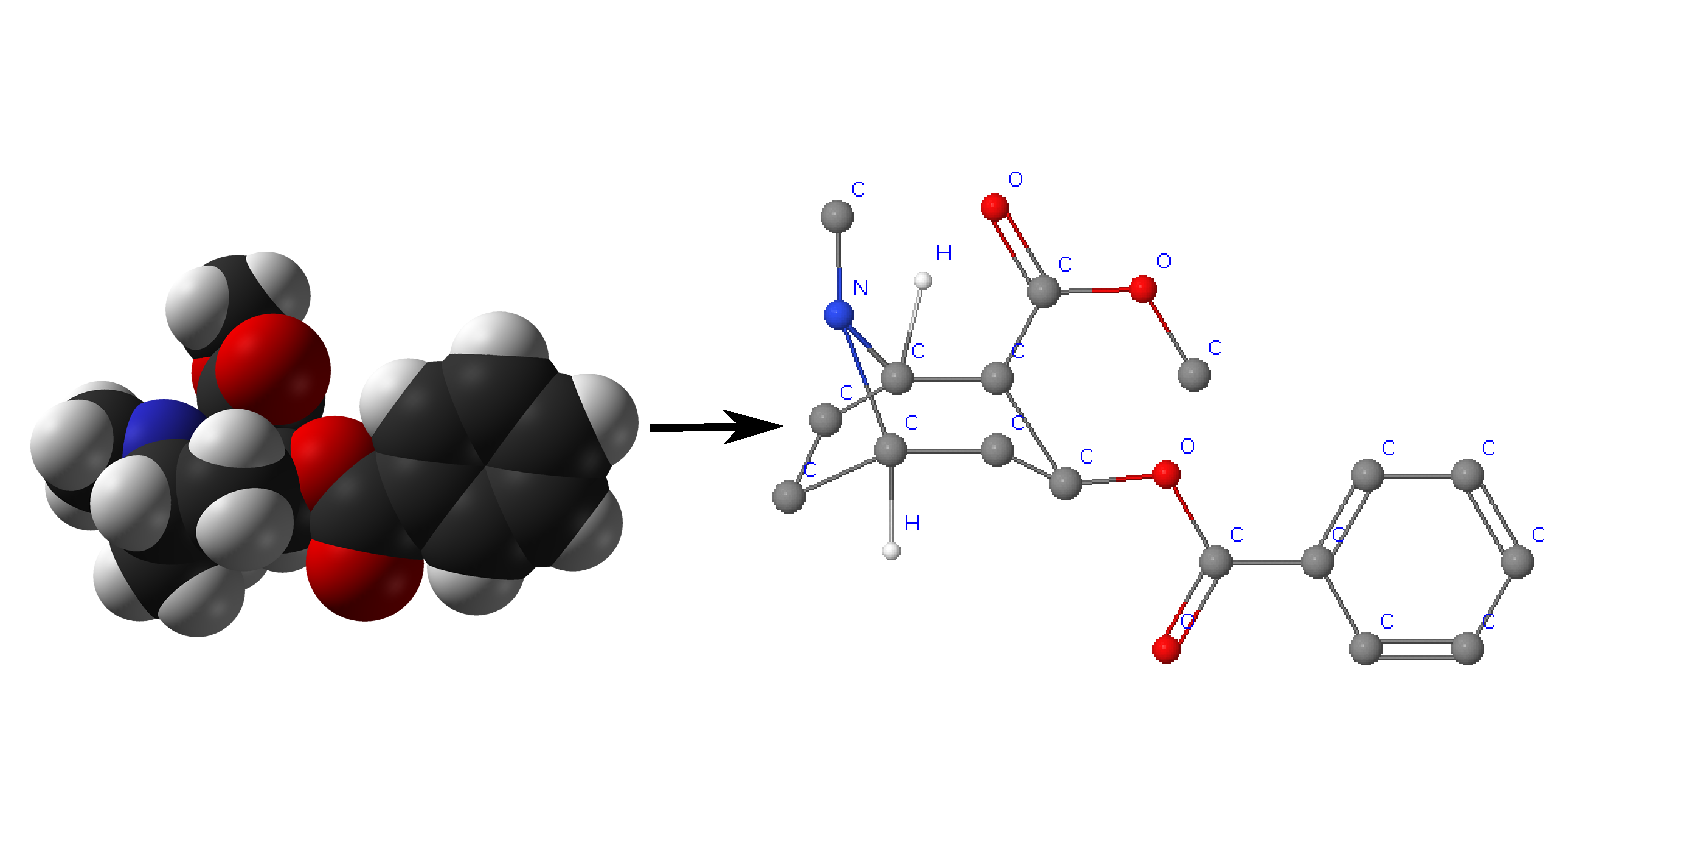
\includegraphics[width=1\columnwidth]{./plots/molecular_graph.pdf}
\put(-9, 5){3D}
\put(-4, 5){2D}
\end{picture}
\caption[Molecular graph representation.]{Example of molecular graph representation, structures are drawn by Jmol. Left, molecular structure of {\em cocaine} is represented as graph in 3D space. Right, the corresponding structure in 2D space.}
\label{molecular_graph}
\end{center}
\end{figure}

% MOL files

The MDL MOL file\footnote{http://www.symyx.com/solutions/white\_papers/ctfile\_formats.jsp} was developed by Symyx\footnote{http://www.symyx.com/}. It is employed in various biochemical databases (eg. KEGG\footnote{http://www.kegg.com/}, PubChem\footnote{http://pubchem.ncbi.nlm.nih.gov/}, ect.) as a standard file format to describe the molecules or chemical objects (eg. proteins, enzymes, etc.). A typical MOL file contains header information, connection table (including atoms and bonds information), and the tail section for identifying the end of a MOL file. It is capable of representing the atoms, bonds, as well the connectivity and relationship of a molecule in a detailed manner. 
% SD file
The structural data file (SDF) format serves as an extension of MOL file format, and can wrap up MOL files of several molecules. The most important feature of SDF file is that the format allow one to contain various properties of molecules (eg. ID, weight, LogP, etc.)

% MOL2 files

Another widely used file format is known as MOL2 file\footnote{http://www.tripos.com/data/support/mol2.pdf}, originated at TRIPOS\footnote{http://www.tripos.com}. Like MOL file format, MOL2 format also contains atoms, bonds, as well as their connectivity and coordinates of a molecule. Besides, it supports partial charge and isotopes. Furthermore, the MOL2 file describe the atom and bond types in a detailed manner which includes substructure information to increase specificity of the atoms and bonds. An example of MOL and MOL2 file formats is shown in Figure~\ref{mol_file}. 

\begin{figure}
\begin{center}
\centering

\setlength{\unitlength}{.4in}
\begin{picture}(11,5)(0,0.5)
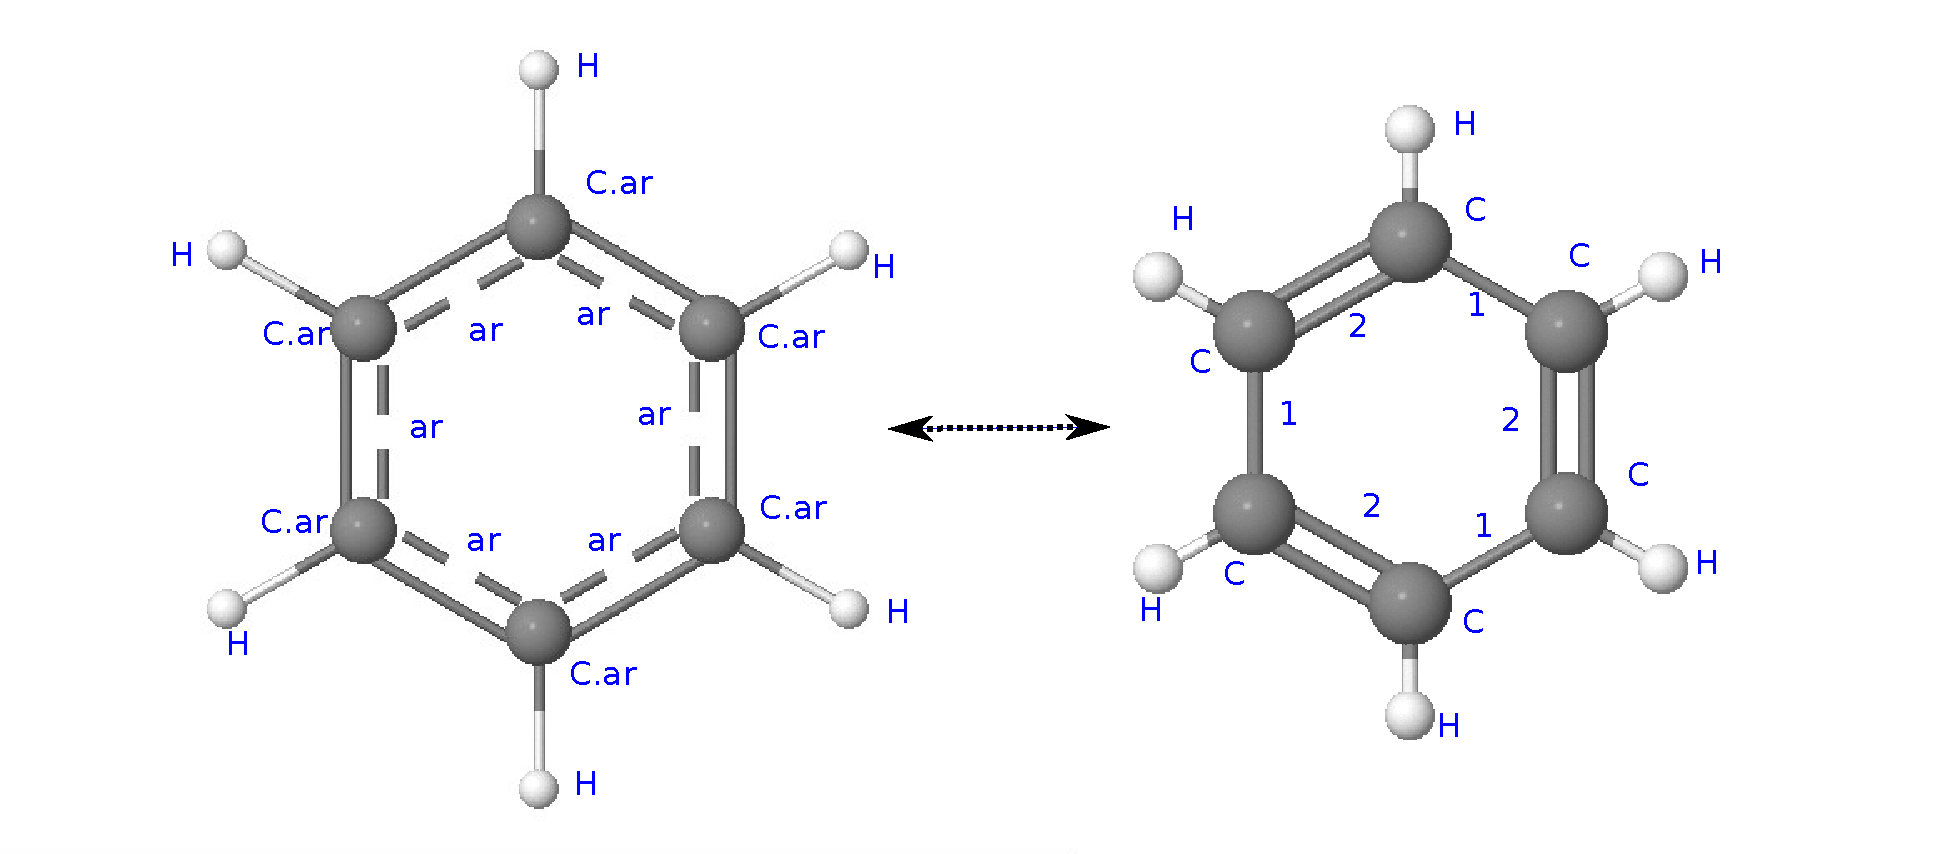
\includegraphics[width=0.80\columnwidth]{./plots/mol_file.pdf}
\put(-3.8,5){MOL}
\put(-9,5){MOL2}
\end{picture}

\caption[MOL1 and MOL2 representations of {\em benzene} molecule.]{Example of MOL and MOL2 formats of {\em benzene}. Left, molecular graph in MOL2 format where {\em aromatic carbon} atoms are explicitly expressed as 'C.ar', and {\em aromatic} bonds are denoted by 'ar'. Right, corresponding graph in MOL format where only simple atom and bond types are supported.}
\label{mol_file}
\end{center}
\end{figure}


\subsection{Reduced graph}

Besides molecular graph, there exists another graph representation of molecules which is known as reduced graph. It is derived from a molecular graph, and initially designed for similarity searching \cite{gillet03}. It is also employed in building structure activity relationship models \cite{barker03}. It only retains the functional structures of a molecule by performing a series of transformations, for example merging nodes that belong to the same functional units. Two kinds of reduction techniques are frequently used, topological pharmacophore reduction and functional group reduction. 

% topological pharmacophore reduction
\subsubsection{Topological pharmacophore reduction}

Topological pharmacophore reduction technique is to collapse nodes in the molecules that represents the set of feature types. The set of feature types was firstly defined in \cite{gillet03}, including ring features and ionization features. Then, it was expanded in \cite{harper} by adding up electron state feature (donor or acceptor) and merging joint features, for example the joint donor-acceptor feature. The complete feature set proposed in \cite{harper} is shown in Table~\ref{tp_feature}. Figure~\ref{tp_reducing} shows an example of topological pharmacophore reduced graph of {\em aspirin} molecule, where features are calculate from JoeLib\footnote{http://www.ra.cs.uni-tuebingen.de/software/joelib/} and the priority of features are ordered according to Table~\ref{tp_feature}.

\begin{center}
\begin{table}\small
\centering
\begin{tabular}{|c|c|c|c|}\hline
\textbf{\em Notation}	&\textbf{\em Ring type}	&\textbf{\em Electron state}	&\textbf{\em Ionization}\\ \hline \hline
Sc &Aromatic &- &- \\ \hline
Ti &Aromatic &Donor &- \\ \hline
V &Aromatic &Acceptor &- \\ \hline
Cr &Aromatic &Donor\&Acceptor &- \\ \hline
Mn &Aromatic &- &Positive \\ \hline
Fe &Aromatic &- &Negative \\ \hline
Co &- &Donor &- \\ \hline
Ni &- &Acceptor &- \\ \hline
Cu &- &Donor\&Acceptor &- \\ \hline
Nb &- &- &Positive \\ \hline
Mo &- &- &Negative \\ \hline
Hf &Aliphatic &Donor &- \\ \hline
Ta &Aliphatic &Acceptor &- \\ \hline
W &Aliphatic &Donor\&Acceptor &- \\ \hline
Re &Aliphatic &- &Positive \\ \hline
Y &Aliphatic &- &Negative \\ \hline
Zr &Aliphatic &- &- \\ \hline
Zn &- &- &- \\ \hline
\end{tabular}
\caption[Topological pharmacophore features.]{Topological pharamacophore features.}
\label{tp_feature}
\end{table}
\end{center} 


\begin{figure}
\begin{center}
\centering

\setlength{\unitlength}{.4in}
\begin{picture}(13,5)(0,1)
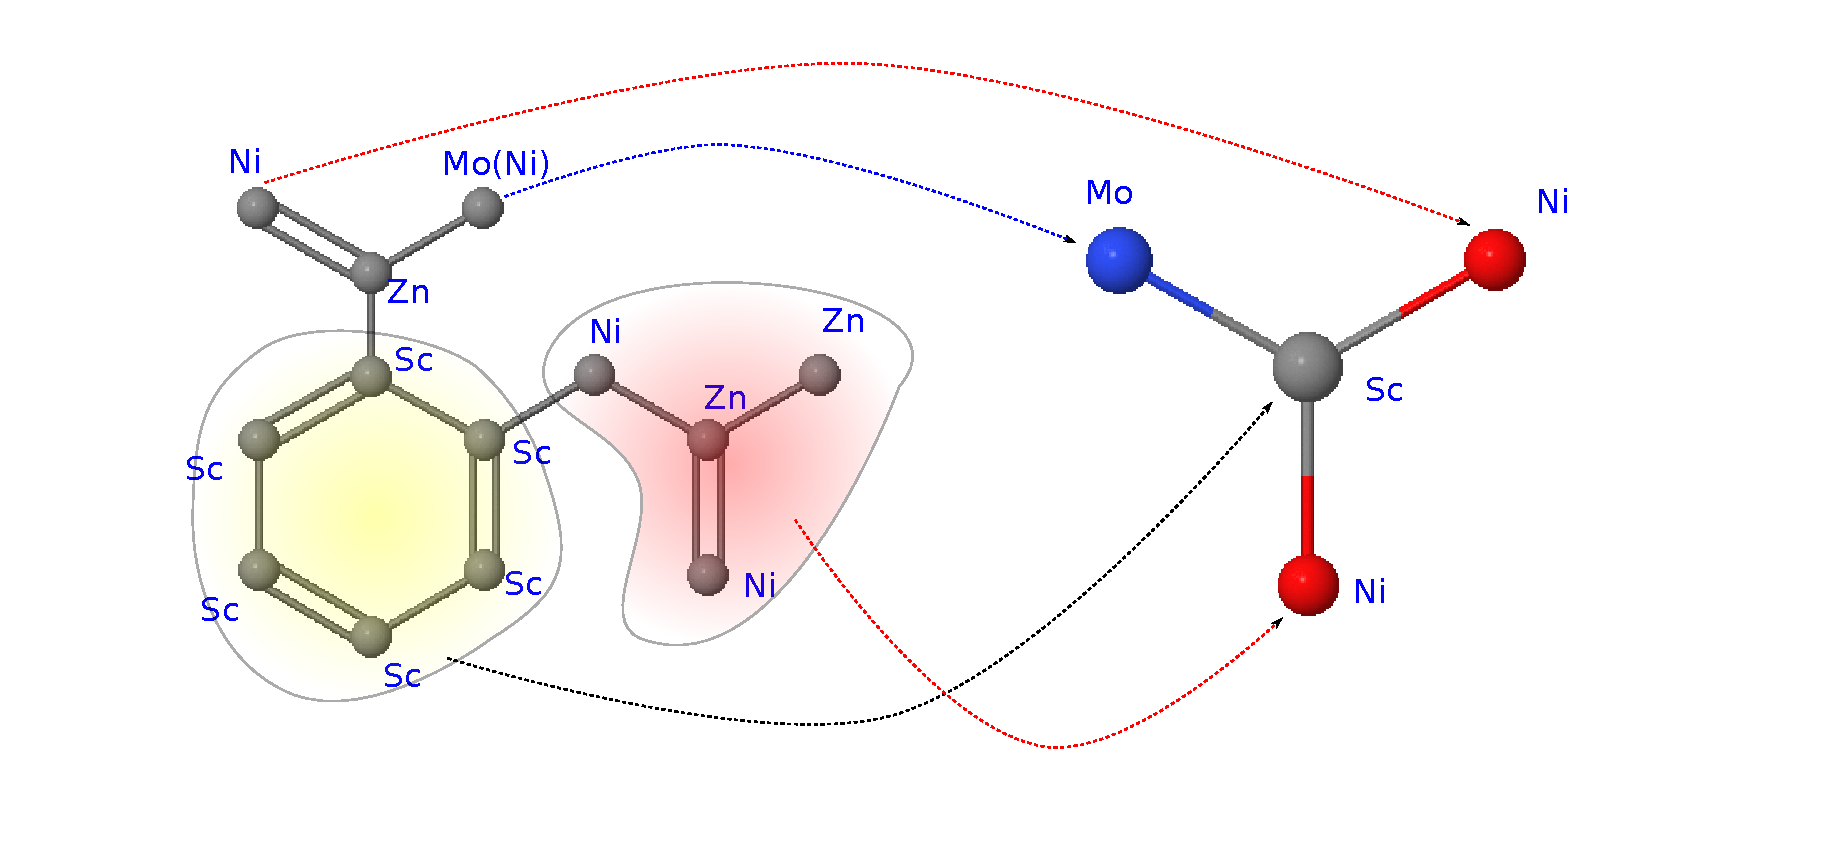
\includegraphics[width=1\columnwidth]{./plots/tp_reducing.pdf}
%\put(0,6){hello}
\end{picture}

\caption[Topological pharmacophore reduction.]{An example of topological pharmacophore reduction. Left, {\em aspirin} molecule labeled by topological pharmacophore features. Topological pharmacophore features are calculated by JoeLib. Right, corresponding reduced graph with feature type {\em Zn} excluded.}
\label{tp_reducing}
\end{center}
\end{figure}

% functional group reducing
\subsubsection{Functional group reduction}

Another reduction technique is based on functional groups, which are specific groups of atoms within molecules that are responsible for chemical properties of those molecules. Functional groups are usually defined by domain experts and therefore have different versions with various size. For example PubChem and OpenBabel have definitions for hundreds of functional groups; on the other hand only $49$ functional groups are employed in \cite{ranu09}. Derived from topological pharmacophore reduction, functional group reduction is to extract atoms in molecules that belong to functional groups and replace them by special notation. Figure~\ref{fg_reducing} demonstrates the functional group reduction of {\em aspirin} molecule based on functional group definition from PubChem\footnote{ftp://ftp.ncbi.nlm.nih.gov/pubchem/specifications/pubchem\_fingerprints.txt}. The priority of functional groups are ordered by size where functional group with more atoms will have higher priority to be extracted. 

\begin{figure}
\begin{center}
\centering

\setlength{\unitlength}{.4in}
\begin{picture}(13,5)(0,1)
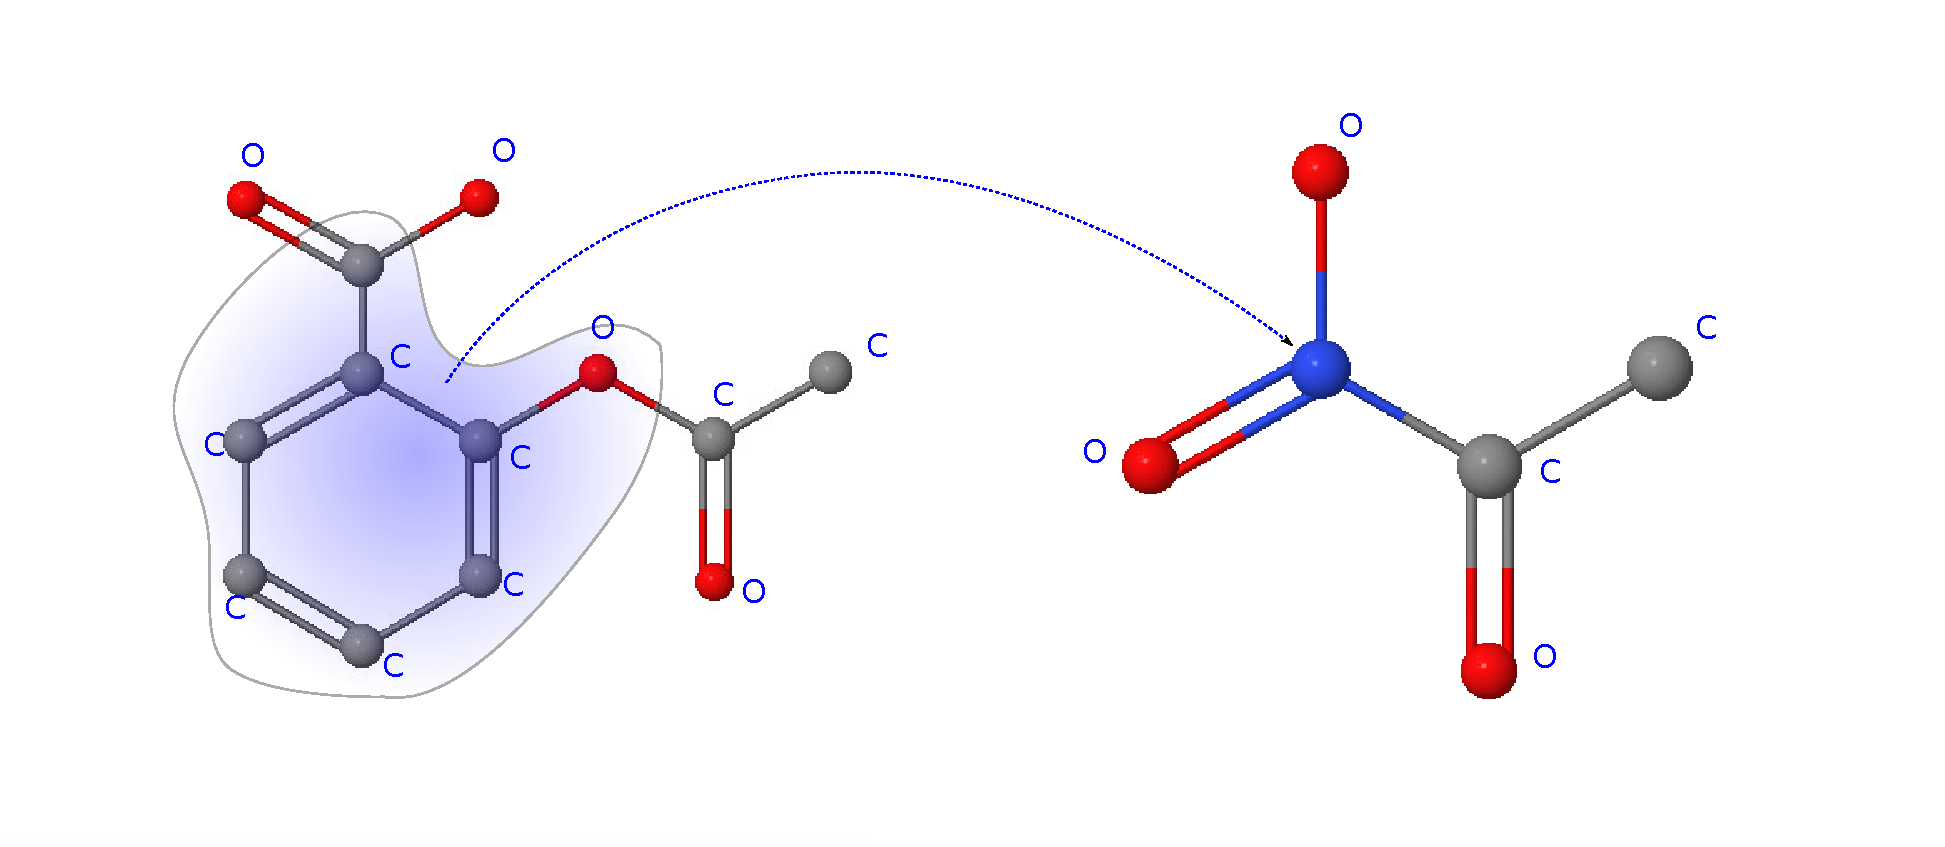
\includegraphics[width=1\columnwidth]{./plots/fg_reducing.pdf}
%\put(0,6){hello}
\end{picture}

\caption[Function group reduction.]{An example of functional group reduction. Left, a functional group with aromatic ring structure is detected in {\em aspirin} molecule. Right, the corresponding reduced graph with functional group being replaced and other atoms being remained.}
\label{fg_reducing}
\end{center}
\end{figure}

% problem with reduced graph
One problem inherited with reduced graph is the order of pharmacophore features or functional groups to be reduced. Different priority strategy will lead to different reduced graph representation of original molecular graph, especially when one atom can be represented by several features or functional groups. For example, one {\em oxygen} atom in Figure~\ref{tp_reducing} represents both acceptor and negative ionization features (Mo and Ni). The priority of feature type Mo is higher than Ni. It therefore be replaced by Mo feature type. Currently, there is no good way to solve the problem except arranging the feature types and functional groups by experts.


\subsection{Molecular descriptors}

Molecular descriptors are designed to encode a molecular structure in a fixed width binary bit vector, which represents the presence or absence of particular substructures or fragments in the molecule. They are extensively used for various tasks in chemical informatics especially for similarity searching, based on the assumption that comparing molecular descriptors will give insight into molecules. There are several variations of molecular descriptors.

\subsubsection{Substructure key}

One kind of fingerprints that was used first is commonly known as {\em substructural key}. It is based on pattern matching of a molecular structure to a set of pre-defined substructures. Each substructure becomes a part of the key and has a fixed position in the descriptor space. These substructures are considered to be independent functional units and are identified based on domain knowledge. Two standards exist for substructure key, MACCS (Molecular Access System) from Symyx and CACTVS \cite{ihlenfeldt94} from PubChem. Figure~\ref{substructure_key} illustrates an example of generation and comparison of substructure keys.

\begin{figure}
\begin{center}
\centering

\setlength{\unitlength}{.4in}
\begin{picture}(12,7.6)(0,-0)
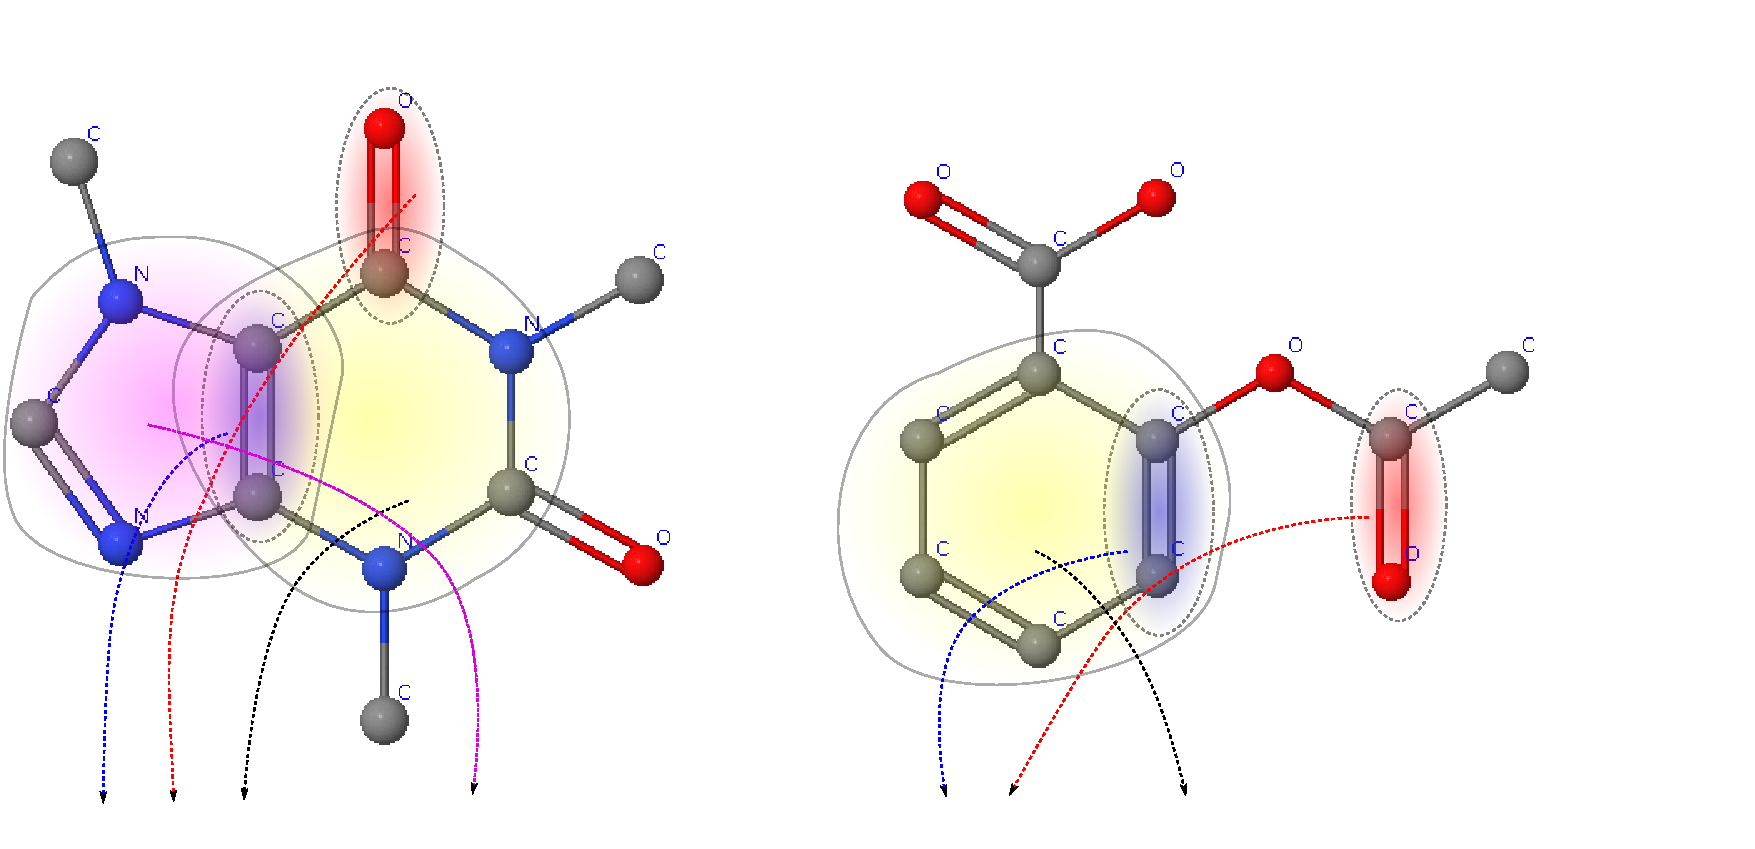
\includegraphics[width=1.0\columnwidth]{./plots/substructure_key.pdf}
\put(-14.5,0){
\begin{tabular}{|c|c|c|c|c|c|} \hline
1 & 1 & 1 & 0 & $\cdots$ & 1 \\ \hline
\end{tabular}
}
\put(-7.3,0){
\begin{tabular}{|c|c|c|c|c|c|} \hline
1 & 1 & 0 & 1 & $\cdots$ & 0 \\ \hline
\end{tabular}
}
\end{picture}

\caption[Molecular fingerprints.]{Example of molecular fingerprints. Two molecules are mapped to bit vectors, where positions correspond to substructures.}
\label{substructure_key}
\end{center}
\end{figure}

However, substructure key suffers from a lack of generality. The substructure set has the critical effect on searching speed as well as the performance of the fingerprints. Substructural keys are usually very sparse since a typical molecule contains just a few substructures.


\subsubsection{Hash fragments} 

An another fingerprint type is called {\em hash fragments}, which enumerates all cycles or linear fragments up to a certain size in the molecule. The size of the fragments is usually bounded between three to seven. A hash function assigns each of the fragments a hash value, which determines its position in descriptor space. As a result, hash fingerprint is capable of encoding a large number of features in a compact manner. Therefore, it circumvents the sparseness of substructural key. DayLight\footnote{http://www.daylight.com/} and OpenBabel\footnote{http://openbabel.org/wiki/} offer molecular fingerprints of hash fragment type.

\subsubsection{Pharmacophore fingerprint}

{\em Pharmacophore fingerprint} is another molecular descriptor that differs from substructure key and hash fragments. It describes the molecules in term of chemical properties other than structural information. In general, it maps molecules to a set of pharmacophore features, each of which has its position in descriptor space like substructure key. The commonly used pharmacophore features include the number of hydrogen bond acceptors (HBA), the number of hydrogen bond donors (HBD), octanol/water partition coefficient (LogP), the number of acidic groups, etc. Molecular descriptors generated from JoeLib\footnote{http://www.ra.cs.uni-tuebingen.de/software/joelib/tutorial/descriptors/descriptors.html} are of the pharmacophore fingerprint type. 




%%%%%%%%%%%%%%%%%%%%%%%%%%%%%%%%%%%%%%%%%%%%%%%%%%%%%%%%%%%%%%%%%%%%%%%%%%%%%%%%%%%%%%%%
%
% Kernels (walk kernel, marginalized walk kernel, weighted decomposition kernel, tanimoto kernel, etc)
%
%%%%%%%%%%%%%%%%%%%%%%%%%%%%%%%%%%%%%%%%%%%%%%%%%%%%%%%%%%%%%%%%%%%%%%%%%%%%%%%%%%%%%%%%

\clearpage
\section{Kernels for drug-like molecules}
\label{kernel_methods_sc}

Kernels computed from the structured representation of molecules extend the scope of the traditional approaches by allowing complex derived features to be used (walks, subgraphs, properties) while avoiding excessive computational cost. In this section, we will review several approaches to construct a graph kernel for classification of drug-like molecules, including walk kernel, decomposition kernel, tree kernel, and descriptor kernels. 


\subsection{Notation}

An {\em undirected graph} $G = (\Vcal, \Ecal)$ is comprised by a set of {\em nodes} $\Vcal$ and set of {\em edges} $\Ecal$. The size of the node set and the edge set are denoted by $|\Vcal|$ and $|\Ecal|$ correspondingly. Different graphs are distinguished by a subscribe $i$, denoted by $G_i = (\Vcal_i, \Ecal_i)$. The node set $\Vcal$ contains a sequence of nodes of finite length, denoted by $\Vcal = \{v_1,v_2,\cdots,v_{|\Vcal|}\}$. A edge is defined as $e = (v_i,v_j)$ and edge set is represented by a finite number of edges denoted by $\Ecal = \{e_1,e_2,\cdots,e_{|\Ecal|}\}$. A {\em walk} of length \(l\) in a graph \(G\) is denoted by \(w = \{v_1,e_1,v_2,e_2,...,v_l\}\) such that for \(i = 1,2,...,{l-1}\) there exists an edge $e_i$ for each pair of nodes \((v_i,v_{i+1})\). 

% matrix notation and some function

The \(n \times n\) adjacency matrix \(E\) of an undirect graph $G$ is defined such that its $(i, j)'\text{th}$ entry $E_{ij}$ equals to one if and only if there is an edge between nodes $v_i$ and $v_j$ (e.g. $(v_i,v_j) \in \Ecal$), and zero otherwise. In an undirected graph, the {\em neighbor set} of a node $v$ is defined by $\delta(v) = \{u \in \Vcal| (v,u) \in \Ecal \vee (u,v) \in \Ecal\}$. The degree of a node $v$ in an undirected graph is represented by $|\delta(v)|$. Furthermore, $\Delta(G)=\text{max}\{|\delta(v)|:v \in \Vcal\}$ represents the {\em maximum degree} of an undirected graph $G$. 






\subsection{Walk kernel}
\label{kernel_methods_walk_kernel_sc}
% marginalized walk kernel - finite walk

The first walk kernel was proposed in \cite{kashima03} as marginalized kernel between labeled graphs. The method measures the similarity between a pair of graphs by means of matching random walks up to an infinite length between them. The longer walks are down-scaled by a probability scheme defined on walks. 

Walk kernel simulates the trajectory of a random $w$ that starts from one node and keeps jumping from one node to its neighbor. Each walk has a starting probability $P_s(w)$ which is the probability of choosing the starting point of the walk. The starting probability is a uniform distribution over all nodes $\Vcal$ in the graph $G$. Subsequently in each step, the walk jumps to the neighbor $v_j$ of current node $v_i$ with the transition probability $P_t(v_j|v_i)$, which is also a uniform distribution over all neighboring nodes of current node. It is also possible that a walk does not jump to the neighbors of current node $v_i$, which requires a stopping probability $P_e(v_i)$. Intuitively, the transition probability $P_t(v_j|v_i)$ and stopping probability $P_e(v_i)$ satisfy the quantitative relation
\begin{align*}
\sum_{j=1}^{m}{P_t(v_j|v_i) + P_e(v_i) = 1},
\end{align*} 
where |$m$| is the number of the neighboring nodes of the current node $v_i$. An example of the probability scheme is shown in Figure~\ref{probability_scheme}. Given a graph $G$, the probability of a random walk is therefore defined as
\begin{align*}
P(w|G) = P_s(v_1) \prod_{i=2}^{l}{P_t(v_i|v_{i-1}) P_e(v_l)},
\end{align*}
where $l$ is the length of the walk $w$.
% TODO constraints

% TODO modify the figure
\begin{figure}
\begin{center}
\centering

\setlength{\unitlength}{.4in}
\begin{picture}(9,7)(0,1.5)
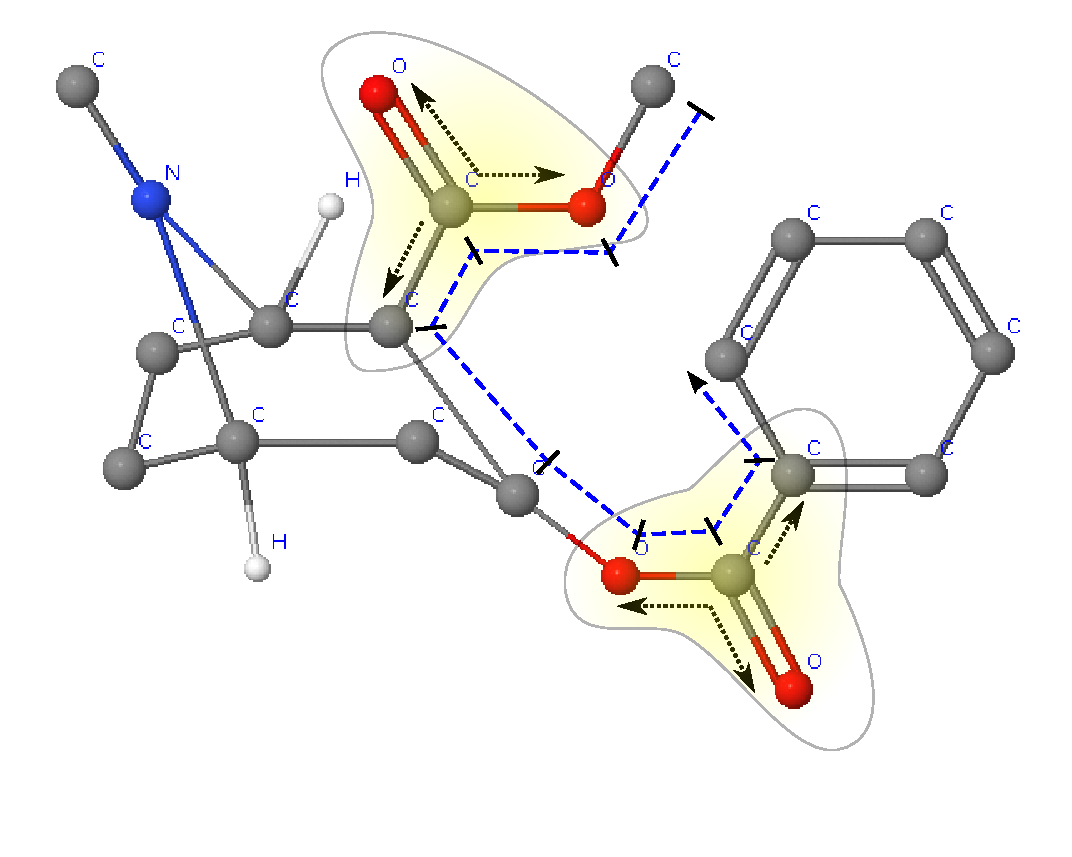
\includegraphics[width=0.70\columnwidth]{./plots/probability_scheme.pdf}
\put(-4,7.9){$P_s(v_1)$}
\put(-4.5,5){$P_e(v_9)$}
\put(-6,7){$P_t(v_j|v_3)$}
\put(-3,2.5){$P_t(v_j|v_7)$}
\end{picture}

\caption[Probability scheme of walk kernel.]{Example of a probability scheme. A random walk of length 9 on {\em Cocaine} molecule is shown as blue dashed line. The starting probability is denoted by $P_s(v_1)$, and the stopping probability by $P_e(v_9)$. The transition probability of an internal nodes $v_i$ in the walk is defined as uniform distribution over all its neighbors shown as yellow areas. For example, transition probabilities of node $v_3$ and $v_7$ are represented by $P_t(v_j|v_3)$ and $P_t(v_j|v_7)$ respectively.}
\label{probability_scheme}
\end{center}
\end{figure}

Next, we define the kernel between two random walks $w$ and $w'$ from pair of graph $G$ and $G'$. Assume $w$ and $w'$  of length $l$ and $l'$are generated according to probability scheme described above. Both of them consists of a sequences of nodes and edges
\begin{align*}
w &= (v_1,e_1,v_2,e_2,\cdots,v_{l-1},e_{l-1},v_l), \\
w' &= (v'_1,e'_1,v'_2,e'_2,\cdots,v'_{l-1},e'_{l-1},v'_l) \nonumber.
\end{align*}
The kernel between a pair of random walks is defined as
\begin{align*}
K_w(w,w') = 
\left\{ 
\begin{array}{l l}
0 & \quad \text{if } l \ne l'\\
K_v(v_1, v'_1)\prod_{i=2}^{l}{K_e(e_i,e'_i)K_v(v_i,v'_i)} & \quad \text{if } l = l'\\
\end{array} \right.,
\end{align*}
where $K_v(v, v')$ and $K_e(e,e')$ are matching kernels defined on pair of nodes and edges which return $1$ if two objects are the same, and $0$ otherwise.

The marginalized walk kernel is summing over the the kernels of all possible pairs of walks up to a infinite length between two graphs, defined as
\begin{align}
K_{mwk}(G_1, G_2) &= \sum_{l=1}^{\infty}\sum_{w_1}\sum_{w_2}{K_w(w_1,w_2)P(w_1|G_1)P(w_2|G_2)},
\label{mwk_def}
\end{align}
where $w_1$ and $w_2$ are random walks of length $l$ in graph $G_1$ and $G_2$.

Computing the kernel $K_{mwk}(G_1, G_2)$ by a straight forward enumeration seems to be impossible, since length of walks range from one to infinite. It is shown in \cite{kashima03} that the kernel function defined by (\ref{mwk_def}) has a nested structure. Therefore, one can calculate the kernel function by an iterative fashion which updates current solution until the function converges.

% produce graph and matrix inversion

Another approach for calculating marginalized walk kernel employs the concept of product graph and matrix inversions. It was introduced in \cite{mahe04} as an extension of marginalized graph kernel. A direct product graph between two labeled undirected graphs \(G_1 = (\Vcal_1,\Ecal_1)\) and \(G_2 = (\Vcal_2,\Ecal_2)\) is denoted by \(G_{\times}(G_1,G_2)\). Node set $\Vcal_{\times}$ and edge set $\Ecal_{\times}$ of are defined as
\begin{align*}
\Vcal_{\times}(G_1,G_2) = &\{(v_1,v_2) \in \Vcal_1 \times \Vcal_2, \text{label}(v_1) = \text{label}(v_2)\},\\
\Ecal_{\times}(G_1,G_2) = &\{((v_1,v_2),(u_1,u_2)) \in \Vcal_\times \times \Vcal_\times, \nonumber \\
	& (v_1,u_1) \in \Ecal_1 \wedge (v_2,u_2) \in \Ecal_2 \wedge \text{label}(v_1,u_1) = \text{label}(v_2,u_2)\}.
\end{align*}
There is a node in the product graph $G_{\times}$ for each pair of nodes from $G_1$ and $G_2$ with the same label. There is an edge in the product graph $G_{\times}$ whenever there are edges in $G_1$ and $G_2$ connecting the corresponding nodes with the same label. An example of a product graph is shown in Figure~\ref{product_graph}. As a result, a walk in product graph corresponds to pair of common walks in the parental graphs.
% TODO graph of product graph
\begin{figure}
\begin{center}
\centering

\setlength{\unitlength}{.4in}
\begin{picture}(12,7)(0,0.5)
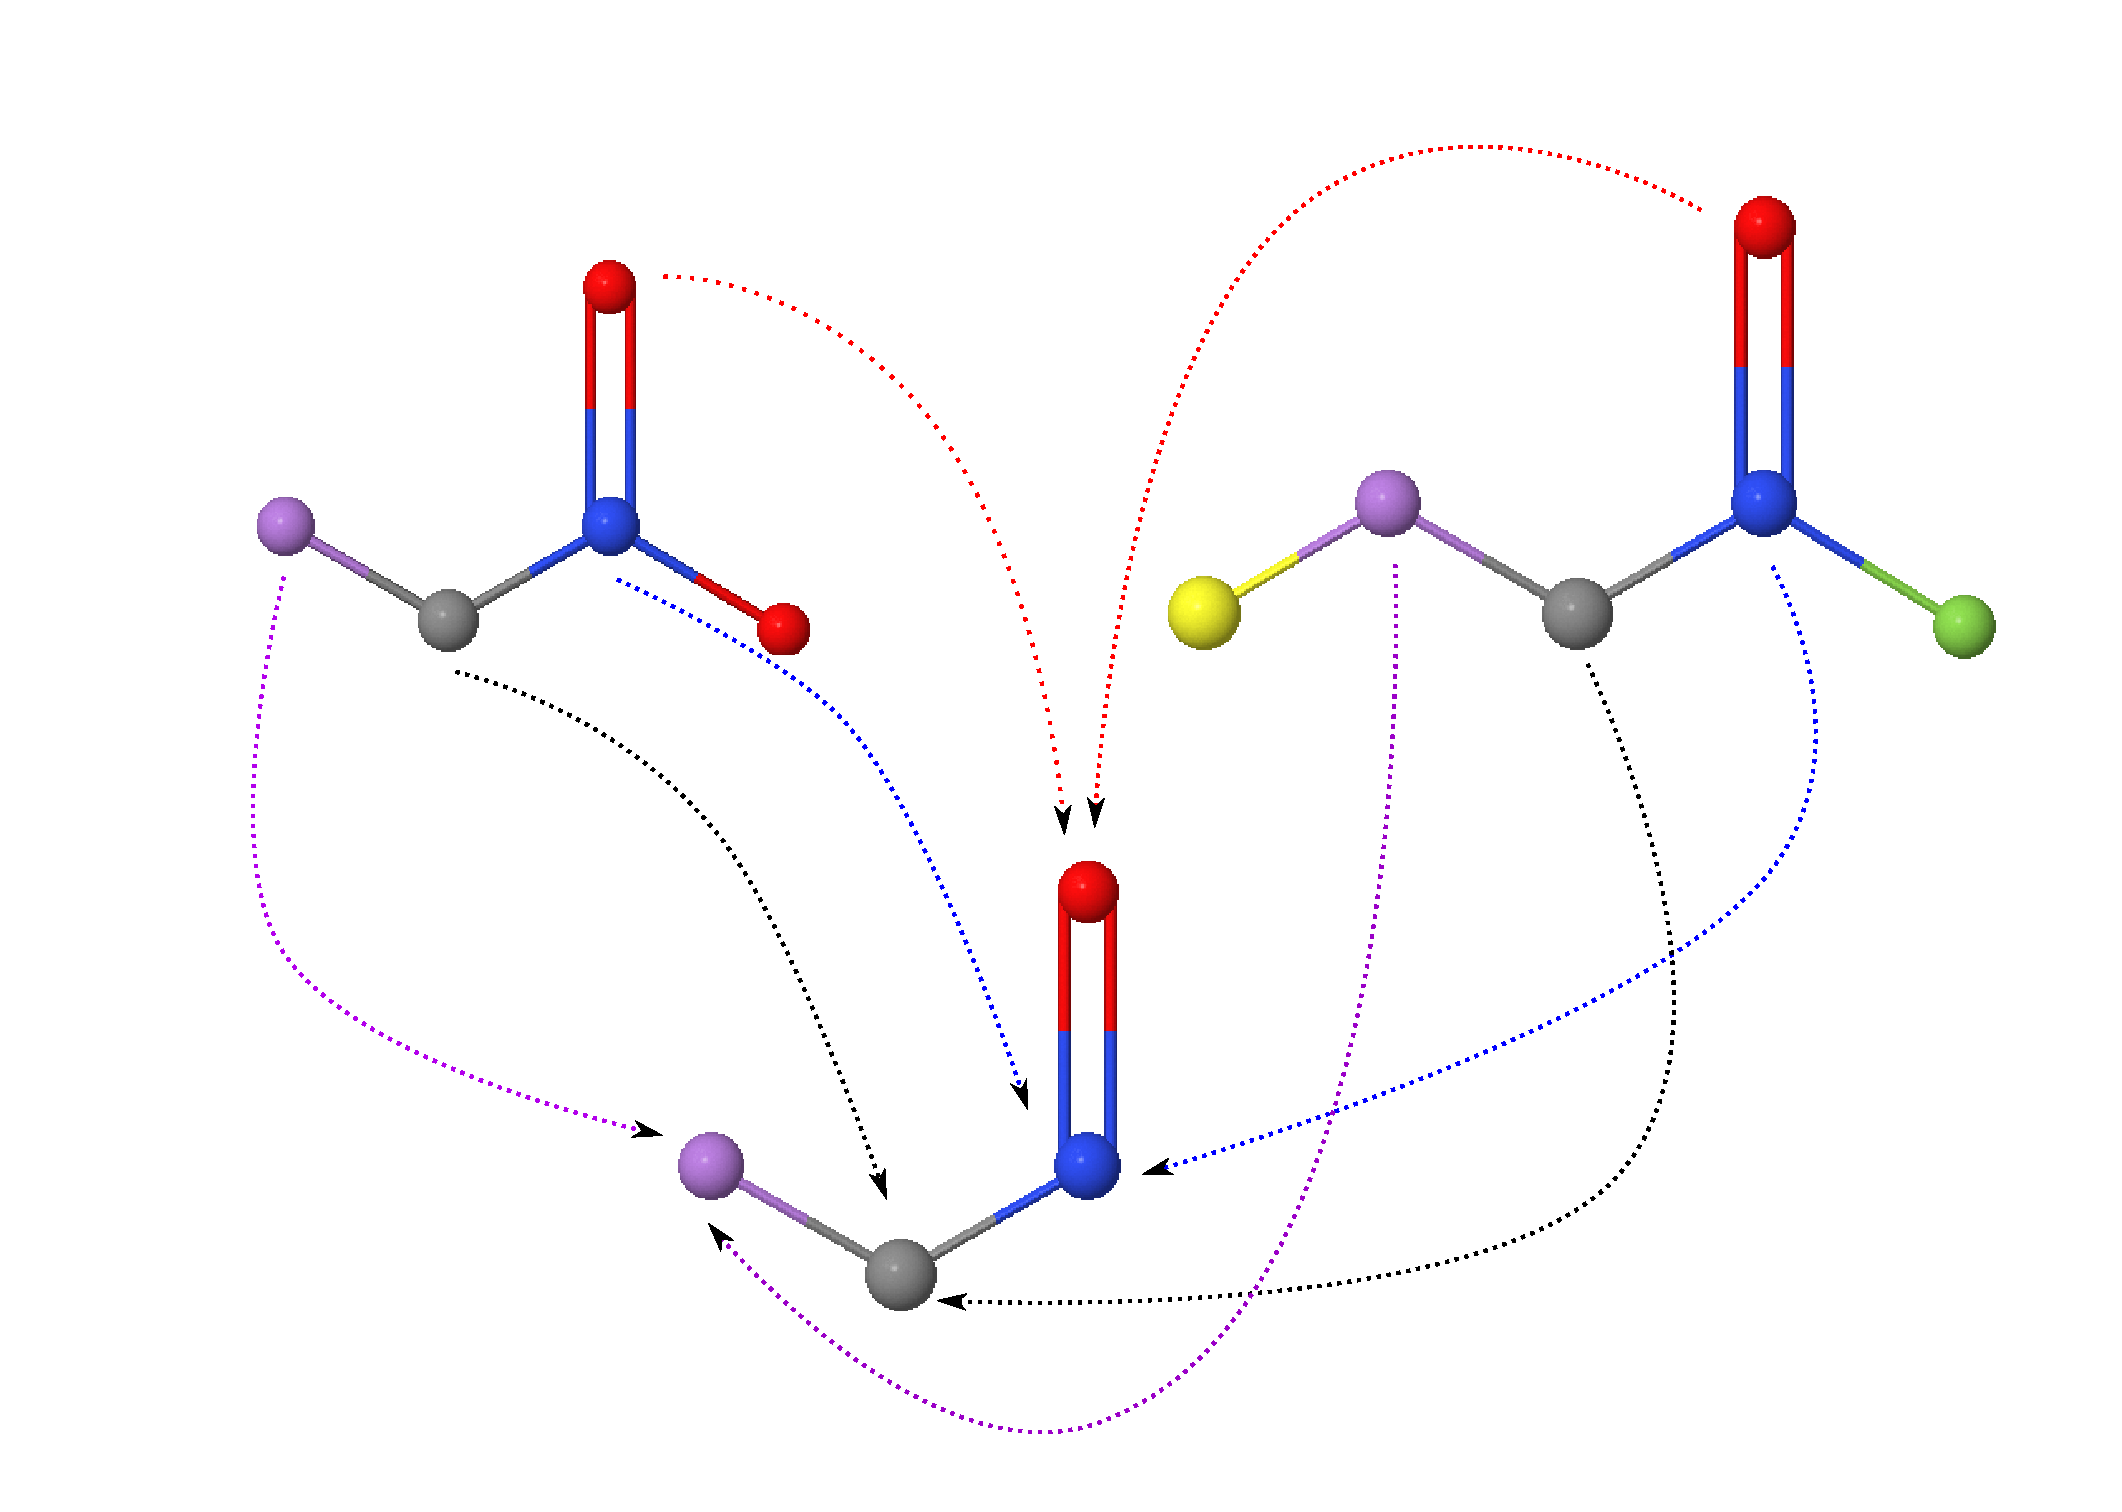
\includegraphics[width=0.80\columnwidth]{./plots/product_graph.pdf}
\put(-9.5,6){$G_1$}
\put(-3,6){$G_2$}
\put(-8.5,1){$G_{\times}$}
\end{picture}

\caption[An example of a product graph.]{Example of product graph. A product graph $G_{\times}$ is constructed from parental graphs $G_1$ and $G_2$. Nodes of different labels are distinguished by different colors. Edge labels are shown as single or double connections. Nodes in $G_1$ are matched with ones in $G_2$. Only matching nodes remained in $G_{\times}$. Edges between matching nodes existing in both $G_1$ and $G_2$ will stay in $G_{\times}$.}
\label{product_graph}
\end{center}
\end{figure}

Given a common walk $w_{\times} = ((v_1,u_2),(v_2,u_2),\cdots,(v_l,u_l))$ of length $l$ in the product graph $G_{\times}$, the probability scheme can be rephrased based on the product graph including a starting probability $\pi_s((v_1,u_1))$, a transition probability $\pi_t((v_i,u_i)|(v_{i-1},u_{i_1}))$, and a stopping probability $\pi_e((v_l,u_l))$ defined as
\begin{align*}
\pi_s((v_1,u_1)) &= P_s(v_1)P_s(u_1), \\
\pi_t((v_i,u_i)|(v_{i-1},u_{i_1})) &= P_t(v_i|v_{i-1})P_t(u_i|u_{i-1}), \\
\pi_e((v_l,u_l)) &= P_e(v_l)P_e(u_l).
\end{align*}
The corresponding probability matrix is denoted by $\pi_s$, $\pi_t$ and $\pi_e$ respectively. The probability of a common walk on product graph is defined by:
\begin{align*}
\pi(w) &= \pi_s((v_1,u_1)) \prod_{i = 1}^{l}{\pi_t((v_i,u_i)|(v_{i-1},u_{i_1}))} \pi_e((v_l,u_l)) = \pi_s \prod_{i = 1}^{l}{\pi_t} \pi_e.
\end{align*}

Then, the kernel function is the summation of every possible walk on the product graph which corresponds to all shared random walks on parental graphs, defined as
\begin{align*}
K_{emk}(G_1,G_2) = \sum_{l=1}^{\infty}\sum_{w}{\pi(w)} = \pi_s^T (I-\pi_t)^{-1} \pi_e^T. 
\end{align*}


% kernel based on adjacency matrix

Besides marginalized walk kernel, there exists another definition of walk kernel as proposed in \cite{gartner03, gartner03a}. The kernel considers the sum of matching walks in a pair of graphs. The contribution of each matching walk is downscaled exponentially according to its length.

The adjacency matrix has an important property which helps us to calculate the number of walks in graph $G$ up to a finite or infinite length. Note that, if the adjacency matrix \(E\) is taken to the power of \(n\), the \((i, j)'\text{th}\) entry \(E_{ij}^n\) shows the number of walks of length \(n\) starting from node \(v_i\) and ending at \(v_j\).

Walk kernel between pair of graph $G_1$ and $G_2$ can be defined based on product graph $G_{\times}(G_1,G_2)$ and its adjacency matrix $E_{\times}$ as:
\begin{align}
K_{wk}(G_1,G_2) = \displaystyle\sum_{i,j = 1}^{\vert \Vcal_{\times} \vert }{\left[\sum_{i=2}^{\infty}{\lambda_i E_\times^n}\right]_{i,j}},
\label{wk_definition_1}
\end{align}
where \(\Vcal_{\times}\) is the node set of the product graph, \(\lambda = (\lambda_1, \lambda_2, \cdots, \lambda_l)\) is the sequence of positive downscaling factor that is strictly less than one, and \(l\) is the length of walk. 

The choice of downscaling factor $\lambda$ allows the walk kernel function take the form of a geometric or an exponential series expansion. It allows us to solve the matrix power series by matrix inversion operation \cite{gartner03} when $l$ is taken to infinity. For example, the limit of a geometric series is:
\begin{align*}
\underset{l \to \infty}{\operatorname{lim}} \, \sum_{i=1}^{l}{\lambda^l} = \frac{1}{1-\lambda},
\end{align*}
where $0<\lambda<1$. The matrix power series takes the form of geometric series when $\lambda_i = \gamma^i$ $(0<\gamma<1)$, and converges if $\gamma<\frac{1}{a}$ where $a \ge \Delta(G_{\times})$. In this case, the limit of matrix power series is given by:
\begin{align*}
\underset{l \to \infty}{\operatorname{lim}} \, \sum_{i=1}^{l}{\lambda^lE^i} = (I-\lambda E)^{-1}.
\end{align*}
where $I$ is identity matrix with ones on diagonal and zeros elsewhere. The matrix inversion operation has a rough cubic time complexity $O(|\Vcal_{\times}|^3)$. We notice that the adjacency matrix $E_{\times}$ is often quite sparse. One can therefore take advantage of methods for sparse matrix to further scale the complexity. However, it is still quite expensive for some molecular graphs. Only several atom types existing in parental graphs makes the size of product graph quite large. 

Since longer walks are downscaled by \(\lambda_i\), the contribution of longer walks are ofter negligible. Figure~\ref{walk_contribution} shows examples of contribution of walks in different length when the matrix power series takes the form of geometric series. Longer walks merely contributes to the final value of the kernel functions. Therefore, we consider finite-length walk kernel where only walks up to length \(l\) are explicitly constructed: 
\begin{align*}
K_{wk}^{l}(G_1,G_2) = \displaystyle\sum_{i,j = 1}^{\vert \Vcal_{\times} \vert }{\left[\sum_{i=2}^{l}{\lambda_i E_\times^n}\right]_{i,j}}.
\end{align*}
Equivalently, it can be defined in a dynamic programming fashion by:
\begin{align}
K_{dwk}^{l}(G_1,G_2) = \sum_{i=1}^{l}\sum_{v_{\times i} \in V_\times}{D_i(v_{\times i})},
\label{wk_definition_2}
\end{align}
where \(D_i(v_i)\) is calculated by:
\begin{align*}
D_0(v_i) &= 1, \\
D_i(v_i) &= \displaystyle\sum_{(v_{\times i},v_{\times j}) \in E_\times}{D_{i-1}(v_{\times j})}.
\end{align*}

% TODO graph of product graph
\begin{figure}
\begin{center}
\centering
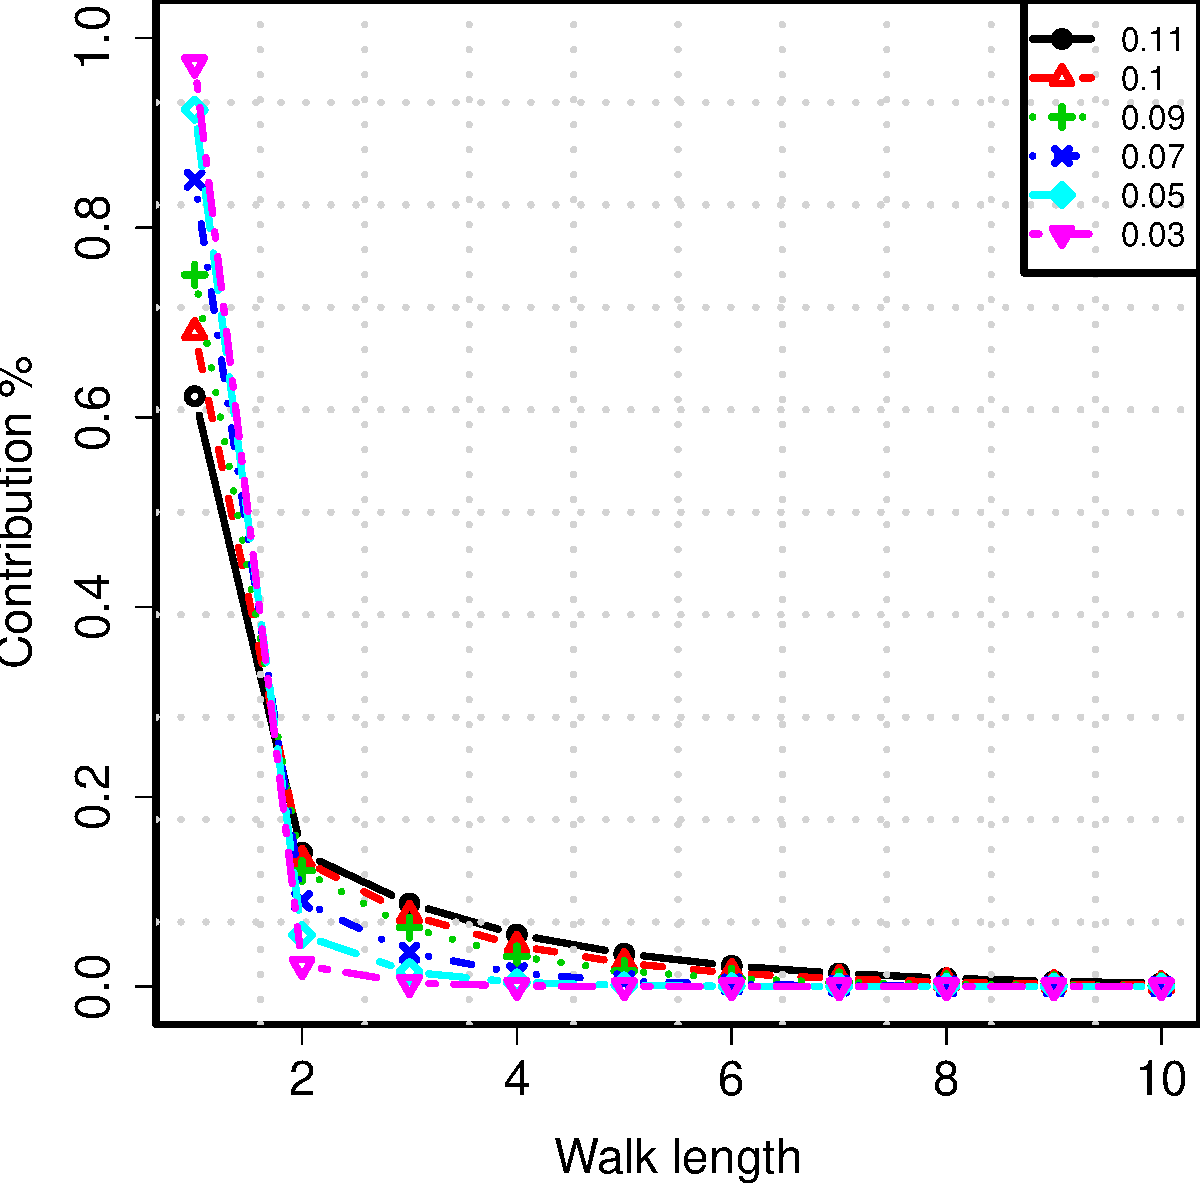
\includegraphics[width=0.70\columnwidth]{./plots/walk_contribution.pdf}
\caption[Contribution of walks in walk kernel.]{Contribution of walks. Here, we considered the walk kernel of two molecules. Molecular structures and the product graph are not shown. The maximum in-degree or out-degree of product graph in this case is $11$. Therefore, the kernel function taking a geometric series form converges when $0<\lambda<\frac{1}{11}$. Walk kernel based on walk of finite length (up to 50) was calculated. The contribution of walks in different length (up to $10$) are explicitly shown as percentage with $\lambda$ ranging from $0.03$ to $0.11$. Longer walks, for example walks of length larger than 8, do not contribution much to kernel function and therefore can be ignored during the calculation.}
\label{walk_contribution}
\end{center}
\end{figure}



%%%%%%%%%%%%%%%%%%%%%%%%%%%%%%%%%%%%%%%%%%%%%%%%%%%%%%%%%%%%%%%%%%%%%%%%%%%%%%%%%%%
\subsection{Weighted decomposition kernel}

Weighted decomposition kernel is an instantiation of convolution kernel \cite{haussler1999} on molecular graphs. It was introduced in \cite{menchetti05} and successfully applied in classification of drug-like molecules in \cite{ceroni07}. Like other convolution kernels, weighted decomposition kernel also relies on the decomposition of a molecular graph into a set of subgraphs and the composition of the kernels from a pair of subgraphs. The kernel between a pair of subgraphs are weighted by means of a exact matching kernel.

Specifically, weighted decomposition kernel is based on a set of decompositions of graph $G$ denoted by $D(s,c,G)$. Selector $s$ corresponds to the atom in graph $G$. $c$ is called contextor, which is the subgraph of $G$ consisting of the surrounding atoms of selector $s$. It is usually defined with parameter $r$, known as contextor radius, as the set of atom that can be reached by selector $s$ by a path with length $r$. An example of graph decomposition is shown in Figure~\ref{decomposition}. 

A weighted decomposition kernel sums over kernels from each pair of contextor defined as
\begin{align}
K_{wdk}(G_1,G_2) = 
\displaystyle\sum_{\substack{v_i,c_i \in D^{-1}(G_1)\\v_j,c_j \in D^{-1}(G_2)}}{\delta(v_i, v_j) K_{sub}(c_i,c_j)},
\label{wdk_definition}
\end{align}
where $D^{-1}(G)$ is inverse function of decomposition operation $D(s_i,c_i,G)$ that returns all tuples $(s_i,c_i)$ satisfying $(s_i,c_i) \in D(s_i,c_i,G)$. $\delta(x_i,x_j)$ is matching kernel defined on pair of selectors and can takes various forms, for example 
\begin{align*}
\delta{(v_i,v_j)} = 
\left\{ 
\begin{array}{l l}
1 & \quad \text{if } v_i = v_j\\
0 & \quad \text{if } v_i \ne v_j\\
\end{array} \right..
\end{align*}
$K_{sub}{(c_i,c_j)}$ is the subgraph kernel that measures the similarity between pair of contextors $c_i$ and $c_j$. The subgraph kernel discards the structural information and focuses the coincident of the attributes in pair of contextors. It is the summary of kernels from individual attribute and can be defined in different form as:
\begin{align*}
K_{sub}(c_i,c_j) &= \sum_{i=1}^{n}{K_{attri}^{i}{(c_i,c_j)}},\\
K_{sub}(c_i,c_j) &= \prod_{i=1}^{n}{K_{attri}^{i}{(c_i,c_j)}},\\
K_{sub}(c_i,c_j) &= \sum_{i=1}^{n}{(1+K_{attri}^{i}{(c_i,c_j))}},
\end{align*}
where $n$ is the number of attributes (eg. atom type, bond type, atom charge, etc.) in the contextor. $K^{i}_{attri}{(c_i,c_j)}$ is the kernel function for the $i$th individual attribute and a variation of histogram interaction kernel. It counts the number of common values in each attribute, defined as
\begin{align*}
K_{attri}^{i}(c_i,c_j) = \displaystyle\sum_{\substack{j = 1}}^{m_i}{\min(p_i(j), {p}_i'(j))},
\end{align*}
where $m_i$ is the number of possible values for attribute $i$, and $p_i(j)$ is the occurrence of value $j$ for attribute $i$. An example of histogram intersection operation related to weighted decomposition kernel is shown in Figure~\ref{intersection}.

\begin{figure}
\begin{center}
\centering

\setlength{\unitlength}{.4in}
\begin{picture}(6,7)(0,0.5)
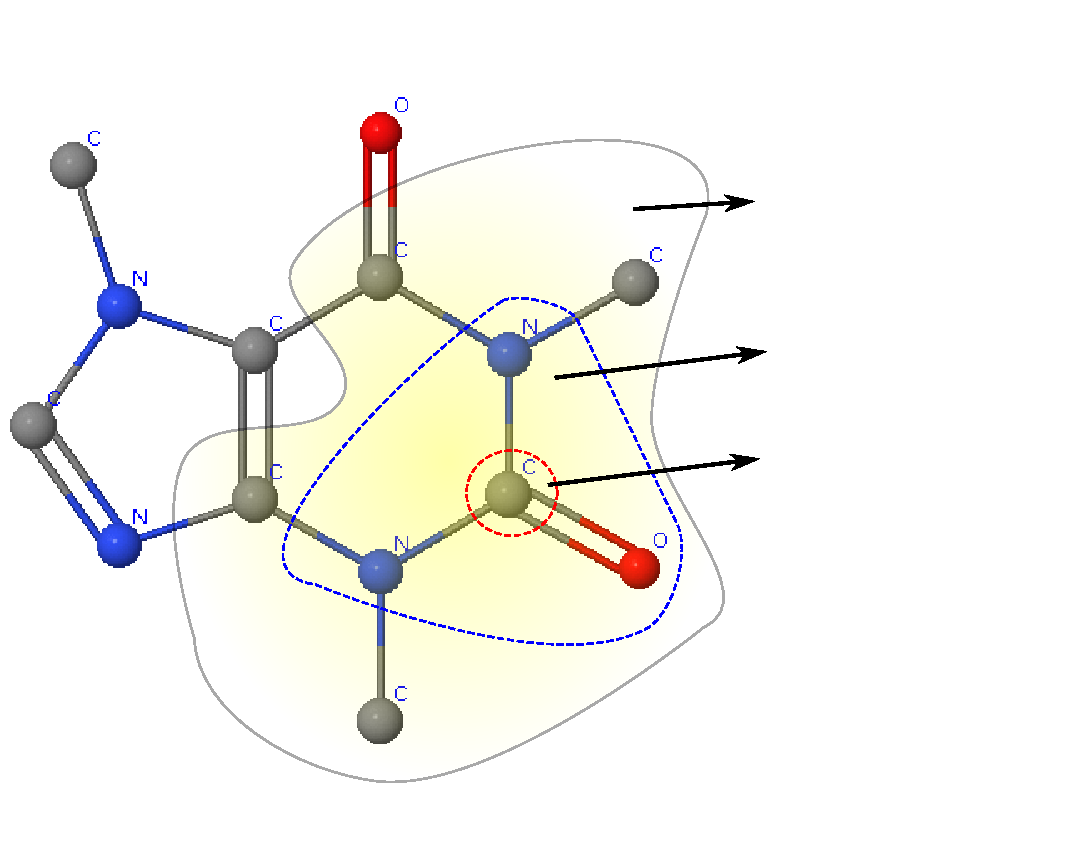
\includegraphics[width=0.60\columnwidth]{./plots/decomposition.pdf}
\put(-2.5,5.3){{\em contextor} $c$, $r = 2$}
\put(-2.5,4.1){{\em contextor} $c$, $r = 1$}
\put(-2.5,3.1){{\em selector} $s$}
\end{picture}

\caption[Graph decomposition.]{Example of graph decomposition. Molecular structure of {\em Caffeine} is shown in figure, where gray atom denotes {\em carbon}, red atom denotes {\em Oxygen} and blue atom denotes {\em nitrogen}. Single or double bonds are also illustrated. A decomposition centers on a {\em carbon} atom shown as selector. The radius $r =1$ contextor and radius $r=2$ contextor are the areas inside the blue curve and the black curve.}
\label{decomposition}
\end{center}
\end{figure}

\begin{figure}
\begin{center}
\centering

\setlength{\unitlength}{.4in}
\begin{picture}(12,9)(0,-2)
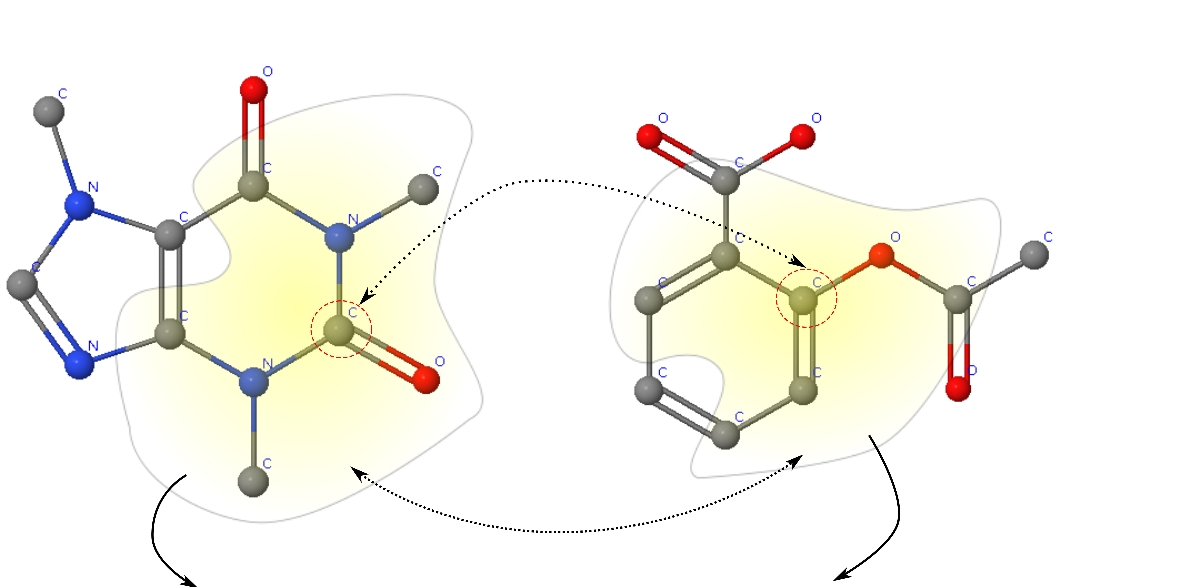
\includegraphics[width=1.0\columnwidth]{./plots/intersection.jpg}
\put(-8.5,5.2){\em selector}
\put(-9,0.3){{\em contextor}, $r=2$}
\put(-13,-1.2){
\begin{tabular}{|c||c|}\hline
{\em Carbon} &   selector\\ \hline
{\em Carbon} &   5\\ \hline
{\em Nitrogen} &   2\\ \hline
{\em Oxygen} &   1\\ \hline
\end{tabular}
}
\put(-7,-1.2){
\begin{tabular}{|c||c|}\hline
{\em Carbon} &   selector\\ \hline
{\em Carbon} &   7\\ \hline
{\em Nitrogen} &   0\\ \hline
{\em Oxygen} &   1\\ \hline
\end{tabular}
}
\end{picture}

\caption[Histogram interaction operation.]{Example of histogram intersection operation. Left is the molecular structure of {\em Caffeine} with one of its radius $r=2$ decomposition. Right is the molecular structure of {\em Aspirin} with one of its $r=2$ decomposition. The histogram of contextors of both molecule is shown in the table. The intersection kernel sums over all three atom types taking the minimum value of both histogram, which is $5+0+1=6$.} 
\label{intersection}
\end{center}
\end{figure}






%%%%%%%%%%%%%%%%%%%%%%%%%%%%%%%%%%%%%%%%%%%%%%%%%%%%%%%%%%%%%%%%%%%%%%%%%%%%%%%%%%%%%%%%%%%%%%%%%5
\subsection{Tanimoto kernel}

Once the molecules are represented as fingerprints, one still need to define the similarity between fingerprints. The similarity measurement should be independent of whether either are hash fingerprints, substructure keys or others. Several kernel functions that measure the similarity of molecular fingerprints were proposed in \cite{ralaivola05} including: {\em Tanimoto kernel, MinMax kernel and Hybrid kernel}. 

Tanimoto kernel, which is derived from Tanimoto coefficient, is specially tailored for measuring the similarity between two binary bit vectors. It is the most popular one among the three and is employed in various chemical toolboxes (eg. OpenBabel\footnote{http://openbabel.org/wiki/}, DayLight\footnote{http://www.daylight.com/}, JoeLib\footnote{http://www.ra.cs.uni-tuebingen.de/software/joelib/}, etc.). 

Given two molecules ${u}$ and ${v}$, as well as the corresponding fingerprints in form of the binary bit vectors $\vphi{(u)}$ and $\vphi{(v)}$ in the same dimension, Tanimoto kernel is defined as
\begin{equation}
K_{TK}(u,v) = 
\displaystyle\frac{(\vphi{(u)} \cdot \vphi{(v)})}{(\vphi{(u)} \cdot \vphi{(u))} + (\vphi{(v)} \cdot \vphi{(v)}) - (\vphi{(u)} \cdot \vphi{(v)})} \, ,
\label{tanimoto_definition}
\end{equation}
where $(\vphi{(u)} \cdot \vphi{(v)})$ denotes the inner product and can be interpreted as the shared 1-bits on two binary vectors $\vphi{(u)}$ and $\vphi{(v)}$. Intuitively, Tanimoto kernel simply measures the ratio between the number of elements in the intersection of two vector $\vphi{(u)}$ and $\vphi{(v)}$ and the number of elements in the union of the two vector $\vphi{(u)}$ and $\vphi{(v)}$. The kernel function returns a value between $0$ and $1$, where $1$ indicates pair of vectors $\vphi{(u)}$ and $\vphi{(v)}$ are identical and $0$ means they are opposite.


%%%%%%%%%%%%%%%%%%%%%%%%%%%%%%%%%%%%%%%%%%%%%%%%%%%%%%%%%%%%%%%%%%%%%%%%%%%%%%%%%%%%%%%%%%%%%%%%%5
\subsection{MinMax kernel}

%TODO: add illustration of molecule with same fingerprints but different structure

Tanimoto kernel is suitable for the cases where molecules are mapped to binary bit vector which corresponds to the present or absent of functional groups, fragments, paths or cycles in the molecules. However, pair of molecules with same binary fingerprints may still vary greatly, for example two molecules with same functional groups but with different numbers. Therefore, using counts other than binary values seems to be more reliable for measuring the similarity between molecules, especially for molecules with different size. The counts in the fingerprint vector indicate the actual number of the objects (eg. paths, cycles, etc.) that exists in the molecules. MinMax kernel \cite{ralaivola05} is designed to meet the need of introducing counts in molecular fingerprints.

Given two molecules $u$ and $v$, and the corresponding fingerprints $\tilde{\vphi}{(u)}$ and $\tilde{\vphi}{(v)}$ with counts in the same dimension, MinMax kernel is defined as
\begin{align*}
K_{MK}(u,v) = 
\displaystyle\frac{\sum_{pos \in \Pcal}{{\bf min}(\tilde{\vphi}{(u)},\tilde{\vphi}{(v)})}}{\sum_{pos \in \Pcal}{{\bf max}(\tilde{\vphi}{(u)},\tilde{\vphi}{(v)})}},
%\label{minmax_definition}
\end{align*}
where {\bf max} and {\bf min} operations result in the vectors that take the maximum or minimum value of each position from two input vector $\tilde{\vphi}{(u)}$ and $\tilde{\vphi}{(v)}$. $\Pcal$ denotes the all positions in fingerprint vector $\tilde{\vphi}{(u)}$.

MinMax kernel works exactly the same as Tanimoto kernel on the molecular fingerprints in form of binary bit vectors. Fingerprints with counts can be translated to an extended fingerprints in form of binary bit vectors by replacing the count in each position with a number of position according to the count. Given two fingerprints $\tilde{\vphi}{(u)}$ and $\tilde{\vphi}{(v)}$ with counts, the transformation $t$ and the corresponding extended fingerprints are defined as
\begin{align}
\tilde{\vphi}{(u)} = (x_{u1},x_{u2},\cdots,x_{un}) \xrightarrow{t} \vphi{(u)} = (\overbrace{y_{11},y_{12},\cdots}^{max(x_{u1},x_{v1})},\overbrace{y_{21},y_{22},\cdots}^{max(x_{u2},x_{v2})},\cdots,\overbrace{y_{n1},y_{n2},\cdots}^{max(x_{un},x_{vn})}),
\label{minmax_transform}
\end{align}
where $x_i \in \mathbb{R}$ and $y_i \in \{0,1\}$. Therefore, MinMax kernel on fingerprints with counts can be interpreted as Tanimoto kernel on the corresponding extended fingerprints, shown in Figure~\ref{minmax_example}. 

\begin{figure}
\begin{center}
\centering
\setlength{\unitlength}{.4in}
\begin{picture}(14,4)(0,0)
\linethickness{1pt}
\put(2,3.6){ $\tilde{\vphi}{(u)}$}
\put(7.5,3.6){ $\tilde{\vphi}{(v)}$}
\put(1.5,3){
\begin{tabular}{|c|c|c|}\hline
3 & 1 & 1 \\ \hline
\end{tabular}
}
\put(7,3){
\begin{tabular}{|c|c|c|}\hline
1 & 3 & 2 \\ \hline
\end{tabular}
}
\put(0,0.6){
\begin{tabular}{|c|c|c|c|c|c|c|c|}\hline
1 & 1 & 1 & 0 & 0 & 1 & 0 & 1  \\ \hline
\end{tabular}
}
\put(5.5,0.6){
\begin{tabular}{|c|c|c|c|c|c|c|c|}\hline
0 & 0 & 1 & 1 & 1 & 1 & 1 & 1  \\ \hline
\end{tabular}
}
\put(2,0){ ${\vphi}{(u)}$}
\put(7.5,0){ ${\vphi}{(v)}$}
\put(10,2.5){ {\footnotesize $K_{MK}(\tilde{\vphi}{(u)},\tilde{\vphi}{(v))} = 0.375$}}
\put(10,1.5){ {\footnotesize $K_{TK}({\vphi}{(u)},{\vphi}{(v))} = 0.375$}}
\put(1.6,2.8){\vector(-3,-4){1.4}}
\put(2.2,2.8){\vector(-1,-3){0.6}}
\put(2.9,2.8){\vector(1,-2){0.9}}
\put(3.3,2.8){\vector(1,-1){1.7}}
\put(7.1,2.8){\vector(-3,-4){1.4}}
\put(7.7,2.8){\vector(-1,-3){0.6}}
\put(8.4,2.8){\vector(1,-2){0.9}}
\put(8.8,2.8){\vector(1,-1){1.7}}
\end{picture}
\caption[An example of MinMax kernel.]{MinMax kernel example. Given two molecules $\ub$ and $\vb$ together with their fingerprints with counts $\tilde{\vphi}{(u)}$ and $\tilde{\vphi}{(v)}$, the value from MinMax kernel function is $0.375$. Transform the fingerprints with counts into ones in form of binary bit vector according to (\ref{minmax_transform}). The similarity between two molecules can be measured equivalently by using Tanimoto kernel over transformed fingerprints $\vphi{(u)}$ and $\vphi{(v)}$.} 
\label{minmax_example}
\end{center}
\end{figure}


\subsection{Hybrid kernel}

Tanimoto kernel focuses on the shared objects in pair of molecules. MinMax kernel considers also the number of shared objects. However, neither of them includes the information about the objects that are absent in both of the molecules. Hybrid kernel \cite{ralaivola05} combines two Tanimoto kernels to measure the number of objects presents in pair of molecules as well as the number of objects that are missing in both of them. Given two molecule $\ub$ and $\vb$ as well as the corresponding fingerprints in form of binary bit vector $\vphi{(u)}$ and $\vphi{(v)}$ in the same dimension, Hybrid kernel is defined as
\begin{align*}
K_{HK}(u,v) = \frac{1}{3}((2-\theta)\cdot K_{TK}(u,v) + (1+\theta)\cdot \neg K_{TK}(u,v)),
%\label{hybrid_definition}
\end{align*}
where $\neg$ is logical negation of binary vector and $\theta \in [-1,+2]$. Hybrid kernel turns to Tanimoto kernel when $\theta=-1$. It should be clear that Hybrid kernel is still valid when replacing Tanimoto kernel with MinMax kernel. It, therefore, works also on the fingerprints with counts.


\subsection{Tree kernel}

Tree kernel was first introduced in \cite{ramon03}, which focus on subtree patterns extracted from graphs. We consider a kernel between two molecular graphs $G_1 = (\Vcal_1,\Ecal_1)$ and $G_2 = (\Vcal_2,\Ecal_2)$. Assume $v_1 \in \Vcal_1$ and $v_2 \in \Vcal_2$, subtrees of height $h$ rooted at $v_1$ and $v_2$ are denoted by $T_{v_1}^h$ and $T_{v_2}^h$. 
% neighbor matching set
A neighbor matching set $\Mcal(v_1,v_2)$ of pair of root nodes in two subtrees $T_{v_1}^h$ and $T_{v_2}^h$ is defined as
\begin{align*}
\Mcal'(v_1,v_2) = \{ &R \subseteq \zeta(v_1) \times \zeta(v_2), R \ne \emptyset \nonumber \\
 & \wedge (\forall(v_a,v_b),(v_c,v_d) \in R, v_a = v_c \Leftrightarrow v_b = v_d) \nonumber \\
 & \wedge (\forall(v_a,v_b)\in R),\text{label}(v_a)=l\text{abel}(v_b) \wedge \text{label}(e_{1a}) = \text{label}(e_{2b}) \},
\end{align*}
where $\zeta(v)$ represents the set of neighbors of node $v$. Each $R \in \Mcal'$ contains identical neighbors of $v_1$ and $v_2$, and corresponds to the tree pattern rooted at $v_1$ and $v_2$ of height $h$ in graph $G_1$ and $G_2$. 

% subtree matching kernel
The subtree matching kernel between pair of subtrees $T_{v_1}^h$ and $T_{v_2}^h$ of height $h$ is defined recursively as:
\begin{align*}
K_{t}^{1}(T_{v_1}^1,T_{v_2}^1) =
\left\{ 
\begin{array}{l l}
1 & \quad \text{if } v_i = v_j\\
0 & \quad \text{if } v_i \ne v_j\\
\end{array} \right.,
\end{align*}
\begin{align*}
K_{t}^{h}(T_{v_1}^h,T_{v_2}^h) = \lambda_{v_1}^h \lambda_{v_2}^h \sum_{R \in \Mcal(v_1,v_2)}\prod_{(v_1',v_2') \in R}{K_{t}^{h-1}(T_{v_1'}^{h-1},T_{v_2'}^{h-1})},
\end{align*}
where $\lambda_v$ is the positive down-scaling factor strictly less than 1. The value $\lambda$ is related to the height of the subtree to ensure that the contributions from bigger trees are balanced with ones from smaller trees.

% tree kernel
Tree kernel between two graph $G_1$ and $G_2$ is defined as
\begin{align*}
K_{tree}(G_1,G_2) = \underset{h \to \infty}{\operatorname{lim}} \, \sum_{v_1 \in V_1}\sum_{v_2 \in V_2}K_{t}^h(T_{v_1},T_{v_2}).
\end{align*}
The kernel sums over all pair of subtrees rooted from each pair of nodes in two graphs. 






%%%%%%%%%%%%%%%%%%%%%%%%%%%%%%%%%%%%%%%%%%%%%%%%%%%%%%%%%%%%%%%%%%%%%%%%%%%%%%%%%%%%%%%%%%%%%%%%%5
%
%	Experimental datasets: Mutag and NCI-cancer
%
%%%%%%%%%%%%%%%%%%%%%%%%%%%%%%%%%%%%%%%%%%%%%%%%%%%%%%%%%%%%%%%%%%%%%%%%%%%%%%%%%%%%%%%%%%%%%%%%%5
\clearpage
\section{Experimental data}

In this section, we will introduce the datasets we employ in our experiments. For NCI-cancer datasets, we will describe the sampling technique we used to construct different version of datasets. We will also describe the auxiliary data, mainly microarray profiling data of cancer cell lines, which we used to construct the Markov network over the cell lines.

\subsection{Mutag dataset}

Mutag dataset is based on data from a review on the literature of mutagenicities in {\slshape Salmonella Typhimurium} based on $230$ aromatic and heteroaromatic nitro compounds \cite{debnath91}. The determinants for mutagenecity in the study were hydrophobicity and energies of the lowest unoccupied molecular orbitals. As a result, $188$ congeners were extracted together with their structure-activity relationship (SAR) data. Therefore, Mutag dataset is very suitable for machine learning and is widely used as one of the standard datasets. 

Specifically, $125$ molecules in Mutag dataset are labeled by $+1$ as positive and \(63\) are labeled by $-1$ as negative. Distribution of molecules in two classes according to the number of atoms and chemical bonds are shown in Figure~\ref{mutag_atom} and Figure~\ref{mutag_bond}. Mutag dataset is publicly available at ChemDB\footnote{ftp://ftp.ics.uci.edu/pub/baldig/learning/mutag/}.

\begin{figure}[h]
\begin{center}
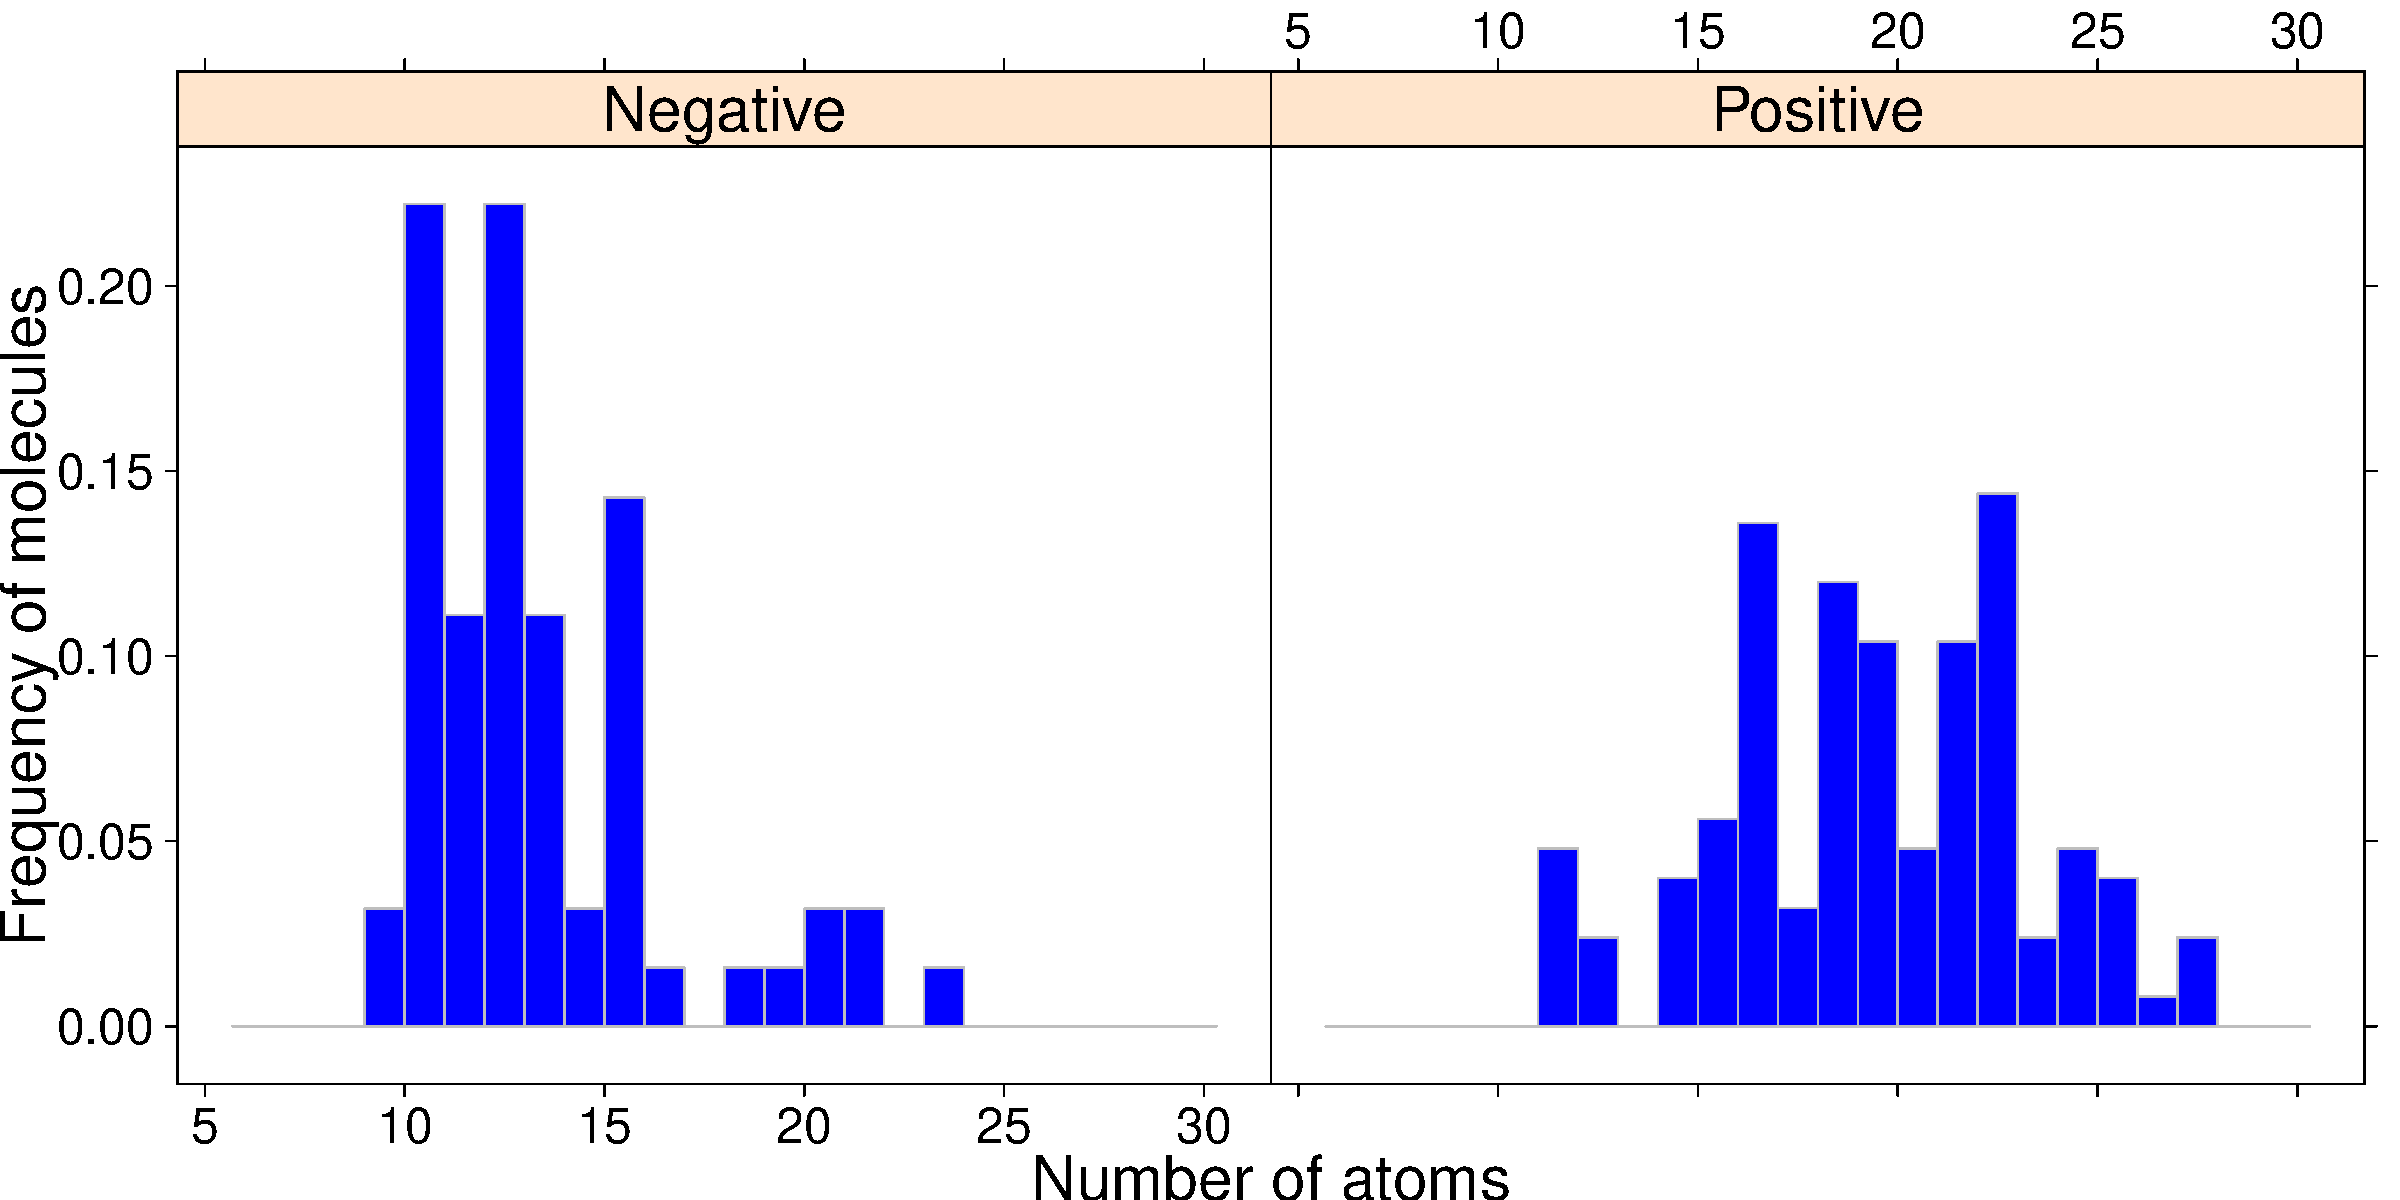
\includegraphics[width=0.9\columnwidth]{./plots/mutag_atom_statistics.pdf}
\caption[Atom distribution of Mutag dataset.]{Distribution molecules according to the number of atoms in Mutag dataset. Left, atom distribution of molecules in negative class. Right, atom distribution of molecules in positive class.}
\label{mutag_atom}
\end{center}
\end{figure}

\begin{figure}[h]
\begin{center}
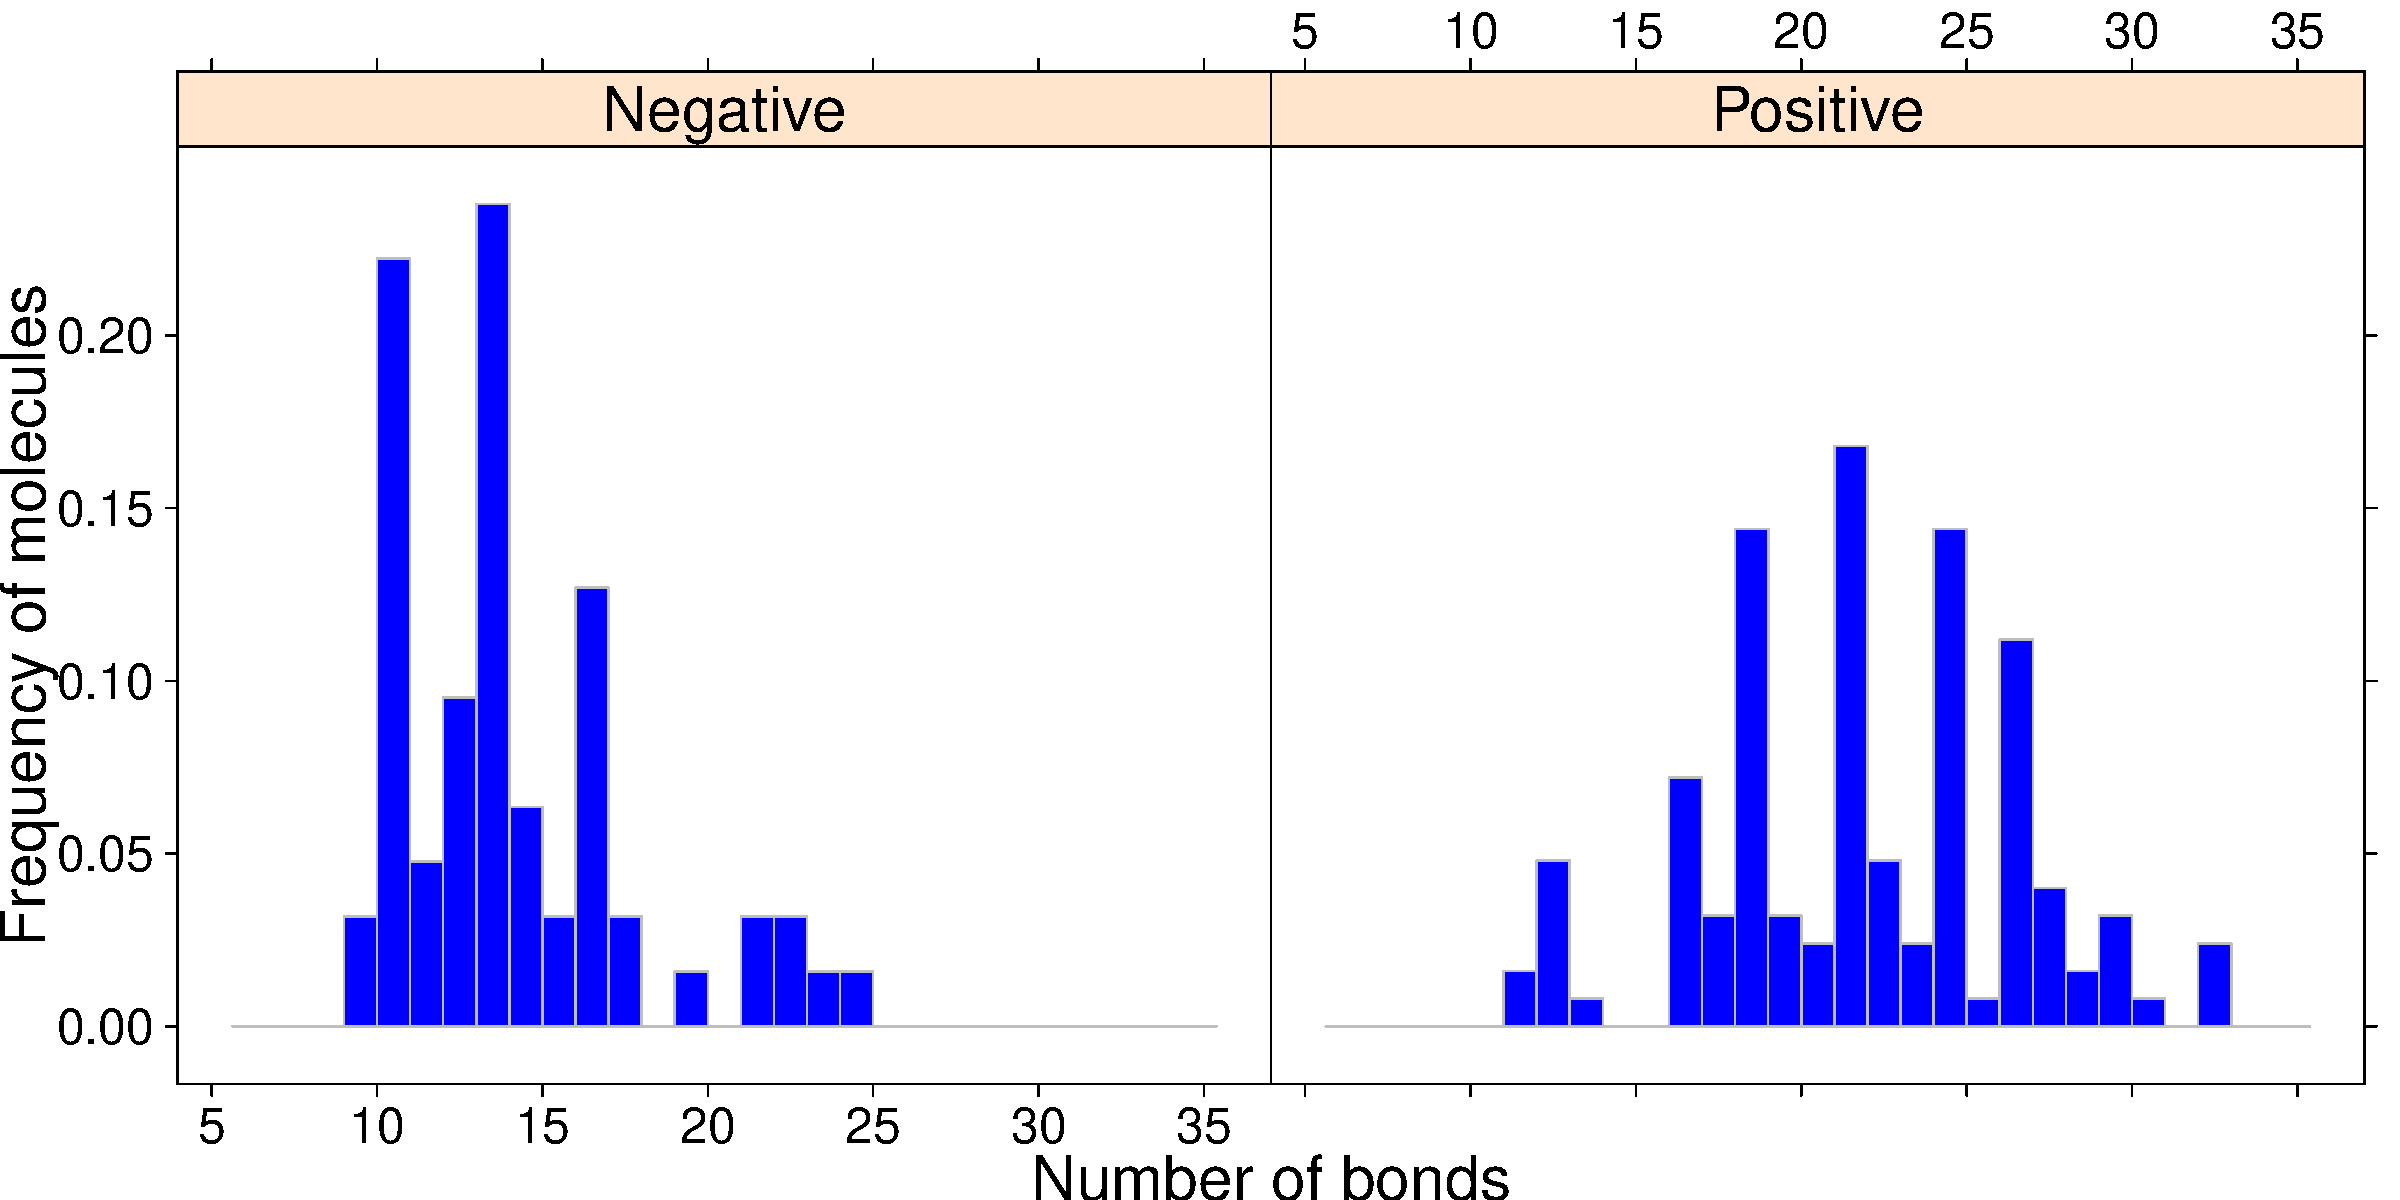
\includegraphics[width=0.9\columnwidth]{./plots/mutag_bond_statistics.pdf}
\caption[Bond distribution of Mutag dataset.]{Distribution of molecules according to the number of bonds in the Mutag dataset. Left, bond distribution of molecules in the negative class. Right, bond distribution of molecules in the positive class.}
\label{mutag_bond}
\end{center}
\end{figure}


\subsection{NCI-cancer datasets}
\label{NCI_cancer_datasets}

Developmental Therapeutics Program\footnote{http://dtp.nci.nih.gov/} (DTP) from National Cancer Institute and National Institutes of Health\footnote{http://www.cancer.gov/} (NCI/NIH) was designed to screen up to \(3,000\) compounds every year searching for potential anti-cancer drugs. This program utilizes bioactivity information of large number of molecules against several human cancer cell lines including leukemia, melanoma and cancers of the lung, colon, brain, ovary, breast, prostate, and kidney. Molecular structure and activity data can be obtained through PubChem Bioassay database\footnote{http://www.ncbi.nlm.nih.gov/pcassay} \cite{wang09b}. For each molecule tested against a certain cell line, the dataset provides a bioactivity outcome that we use as the classes (active, inactive).

NCI-cancer datasets were first employed in early study \cite{swamidass05} of predicting mutagenecity, toxicity and anti-cancer activity by independently sampling for each subset approximately equivalent number of active molecules and inactive ones from original datasets. The datasets resulted from sampling were mostly used in the subsequent researches. However, we found the sampled datasets were erroneous and lots of molecules were mislabeled compared to the latest version of PubChem Bioassay database. Therefore, we discard the old datasets and reconstruct the datasets that was employed in the following experiments. The reconstruction is directly based on PubChem Bioassay database.

Currently, there are \(43,884\) molecules in the PubChem Bioassay database together with anti-cancer activities in \(73\) cell lines. \(59\) cell lines have screening experimental results for most molecules and $4,554$ molecules have no missing data in these cell lines, therefore these cell lines and molecules are selected and employed in our experiments. The number of active molecules as well as inactive ones in each subset of NCI-cancer datasets are reported in Table~\ref{cancer_statistics}.

\begin{center}
\begin{table}
\centering
\begin{tabular}{|c|c|c||c|c|c|}\hline
%\textbf{\em Cell line}	&\textbf{\em Active}	&\textbf{\em Inactive}	&\textbf{\em Active \%}	&\textbf{\em Cell line}	&\textbf{\em Active}	&\textbf{\em Inactive} &\textbf{\em Active \%}	\\ \hline \hline
\textbf{\em Cell line}	&\textbf{\em Active}	&\textbf{\em Inactive}	&\textbf{\em Cell line}	&\textbf{\em Active}	&\textbf{\em Inactive}	\\ \hline \hline

NCI-H23& 831& 3723 &NCI-H226& 711& 3843 \\ \hline
NCI-H322M& 647& 3907 &NCI-H460& 953& 3601 \\ \hline
HOP-62& 760& 3794 &HOP-92& 743& 3811 \\ \hline
NCI-H522& 1104& 3450 &A549/ATCC& 765& 3789 \\ \hline
EKVX& 599& 3955 &LOX-IMVI& 1005& 3549 \\ \hline
M14& 863& 3691 &MALME-3M& 823& 3731 \\ \hline
UACC-62& 861& 3693 &UACC-257& 677& 3877 \\ \hline
SK-MEL-2& 678& 3876 &SK-MEL-5& 903& 3651 \\ \hline
SK-MEL-28& 621& 3933 &PC-3& 783& 3771 \\ \hline
DU-145& 733& 3821 &SF-268& 804& 3750 \\ \hline
SF-295& 806& 3748 &SF-539& 852& 3702 \\ \hline
SNB-19& 661& 3893 &SNB-75& 760& 3794 \\ \hline
U251& 866& 3688 &HT29& 857& 3697 \\ \hline
COLO205& 863& 3691 &HCT-15& 859& 3695 \\ \hline
KM12& 808& 3746 &HCC-2998& 765& 3789 \\ \hline
HCT-116& 1002& 3552 &SW-620& 979& 3575 \\ \hline
MCF7& 1027& 3527 &MDA-MB-435& 899& 3655 \\ \hline
MDA-N& 888& 3666 &BT-549& 670& 3884 \\ \hline
T-47D& 759& 3795 &NCI/ADR-RES& 706& 3848 \\ \hline
MDA-MB-231& 681& 3873 &HS-578T& 685& 3869 \\ \hline
OVCAR-3& 859& 3695 &IGROV1& 801& 3753 \\ \hline
SK-OV-3& 634& 3920 &OVCAR-4& 631& 3923 \\ \hline
OVCAR-5& 558& 3996 &OVCAR-8& 858& 3696 \\ \hline
RPMI-8226& 1074& 3480 &SR& 1357& 3197 \\ \hline
CCRF-CEM& 1377& 3177 &K-562& 1144& 3410 \\ \hline
MOLT-4& 1207& 3347 &HL-60(TB)& 1321& 3233 \\ \hline
A498& 663& 3891 &CAKI-1& 827& 3727 \\ \hline
RXF393& 836& 3718 &786-0& 908& 3646 \\ \hline
ACHN& 848& 3706 &TK-10& 578& 3976 \\ \hline
UO-31& 766& 3788 && & \\ \hline

\end{tabular}
\caption[NCI-cancer dataset with full data.]{Number of active and inactive molecules in NCI-cancer datasets with all molecules.}
\label{cancer_statistics}
\end{table}
\end{center}

However, molecular activity data are highly biased over the cell lines. Figure~\ref{activity_hist} shows the molecular activity distribution over all 59 cell lines. Most of the molecules are inactive in all cell lines, while a relatively large proportion of molecules are active against almost all cell lines, which can be taken as toxics. These molecules are less likely to be potential drug candidates than the ones in the middle part of the histogram. 

\begin{figure}[t]
\begin{center}
\centering
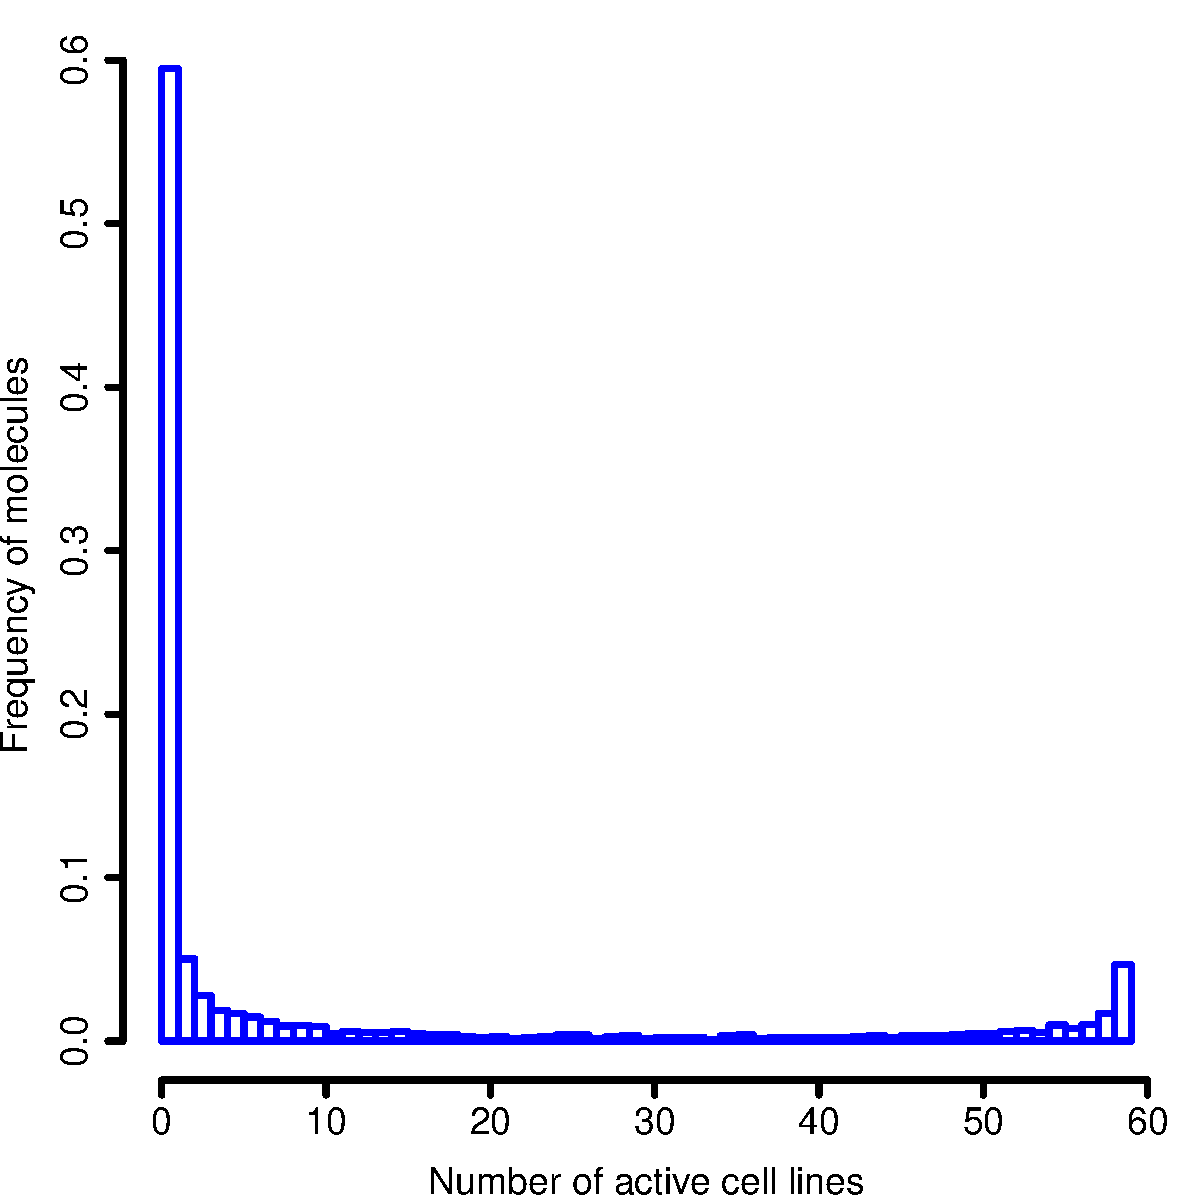
\includegraphics[width=0.60\columnwidth]{./plots/activity_hist.pdf}
\caption[Skewness of multilabel distribution.]{Skewness of the multilabel distribution. Molecules are sorted according to the number of cell lines they are active against, from zero to 59. Label on the x-axis denotes the number of cell lines that molecules are active against.}
\label{activity_hist}
\end{center}
\end{figure}

Figure~\ref{kernel_heatmap} shows a heatmap of a normalized Tanimoto kernel, where molecules have been sorted by the number of cell lines they are active against. The heatmap shows that the molecules in the two extremes of the multilabel distribution form groups of high similarity whereas the molecules in the middle are much more dissimilar both to each other and to the extreme groups. The result seems to indicate that the majority of molecules in the dataset are either very specific or very general in the targets they are active against.  Other kernels mentioned in section \ref{kernel_methods_sc} produce a similar heatmap indicating that the phenomenon is not kernel-specific.

\begin{figure}
\begin{center}
\centering
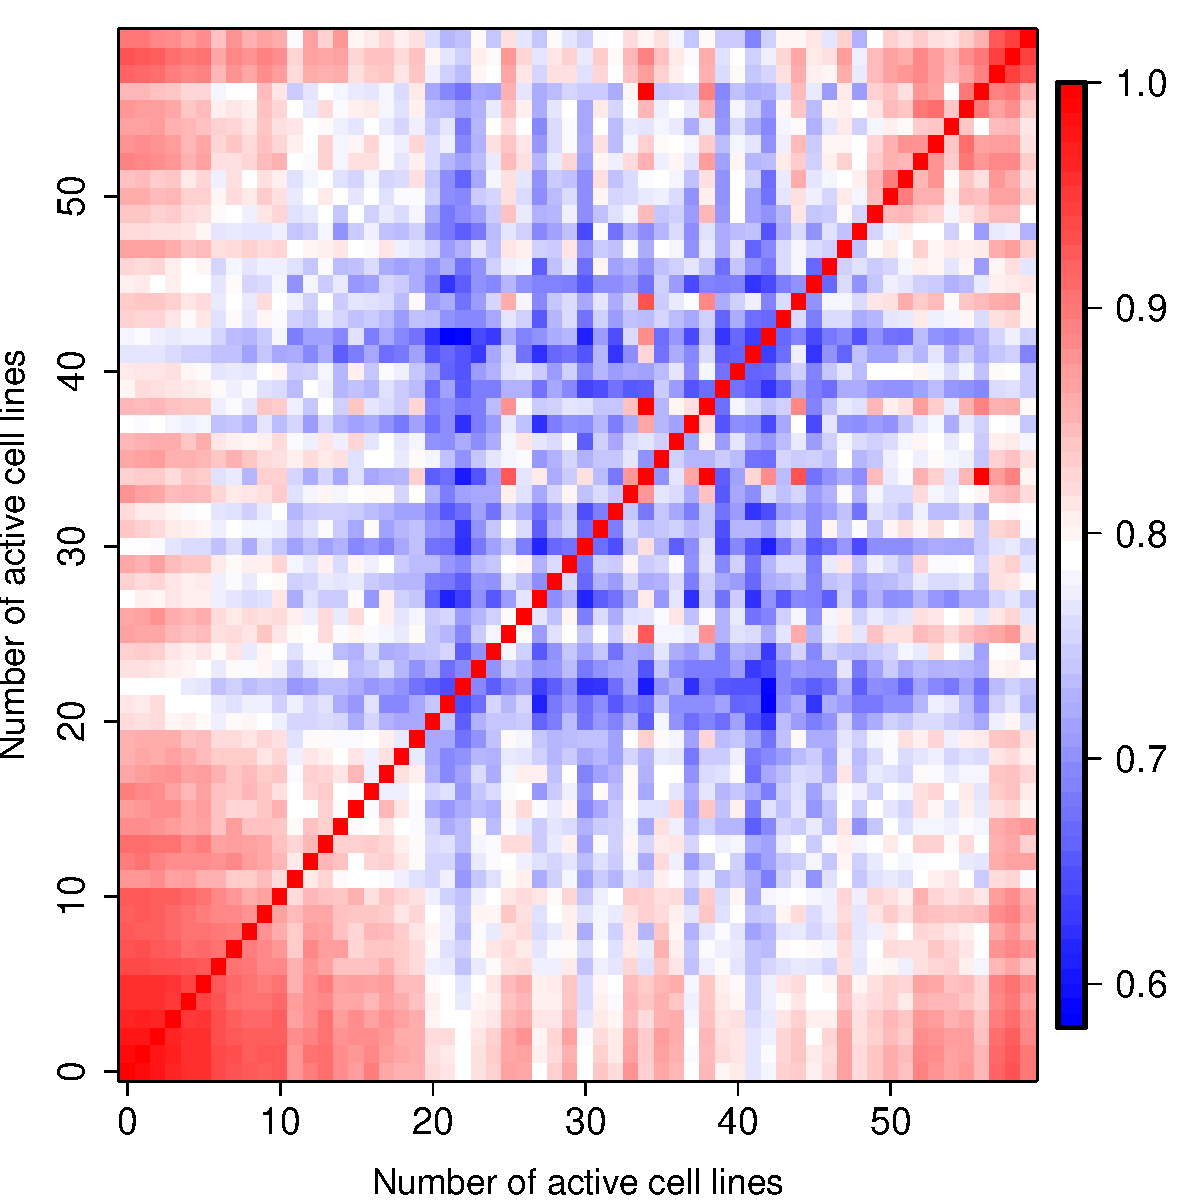
\includegraphics[width=0.6\columnwidth]{./plots/kernel_heatmap.pdf}
\caption[Heatmap of kernel space.]{Heatmap of the kernel space for the molecules sorted by the multilabel distribution. Label on axises denotes the number of cell lines that molecules are active against.}
\label{kernel_heatmap}
\end{center}
\end{figure}

Because of the above-mentioned skewness, we prepared different versions of the dataset:
\begin{description}
  \item[Full.] This dataset contains all $4,554$ molecules from the NCI-cancer dataset with their activity class (active vs. inactive) recorded against all $59$ cancer cell lines.

  \item[No-Zero-Active.] In this dataset, we removed all molecules that are not active towards any of the cell lines (corresponding to the leftmost peak in Figure \ref{activity_hist}). The remaining $2,305$ molecules are all active against at least one cell line. The number of the molecules that are active or inactive against each subsets of the dataset is shown in Table~\ref{cancer_statistics_1}.

  \item[Middle-Active.] In order to circumvent the skewness and concentrate on the most interesting molecule, we also followed the preprocessing procedure suggested in \cite{shivakumar09}, and selected the molecules that are active against more than \(10\) cell lines and inactive against more than \(10\) cell lines. Middle-active means the molecules that are active against average number of cell lines. As a result, \(544\) molecules remained and were employed in our experiments. The number of active and inactive molecules in dataset of this version is shown in Table~\ref{cancer_statistics_2}.
\end{description}


\begin{center}
\begin{table}
\centering
\begin{tabular}{|c|c|c||c|c|c|}\hline
%\textbf{\em Cell line}	&\textbf{\em Active}	&\textbf{\em Inactive}	&\textbf{\em Active \%}	&\textbf{\em Cell line}	&\textbf{\em Active}	&\textbf{\em Inactive} &\textbf{\em Active \%}	\\ \hline \hline
\textbf{\em Cell line}	&\textbf{\em Active}	&\textbf{\em Inactive}	&\textbf{\em Cell line}	&\textbf{\em Active}	&\textbf{\em Inactive}	\\ \hline \hline

NCI-H23& 831& 1474 &NCI-H226& 711& 1594 \\ \hline
NCI-H322M& 647& 1658 &NCI-H460& 953& 1352 \\ \hline
HOP-62& 760& 1545 &HOP-92& 743& 1562 \\ \hline
NCI-H522& 1104& 1201 &A549/ATCC& 765& 1540 \\ \hline
EKVX& 599& 1706 &LOX-IMVI& 1005& 1300 \\ \hline
M14& 863& 1442 &MALME-3M& 823& 1482 \\ \hline
UACC-62& 861& 1444 &UACC-257& 677& 1628 \\ \hline
SK-MEL-2& 678& 1627 &SK-MEL-5& 903& 1402 \\ \hline
SK-MEL-28& 621& 1684 &PC-3& 783& 1522 \\ \hline
DU-145& 733& 1572 &SF-268& 804& 1501 \\ \hline
SF-295& 806& 1499 &SF-539& 852& 1453 \\ \hline
SNB-19& 661& 1644 &SNB-75& 760& 1545 \\ \hline
U251& 866& 1439 &HT29& 857& 1448 \\ \hline
COLO205& 863& 1442 &HCT-15& 859& 1446 \\ \hline
KM12& 808& 1497 &HCC-2998& 765& 1540 \\ \hline
HCT-116& 1002& 1303 &SW-620& 979& 1326 \\ \hline
MCF7& 1027& 1278 &MDA-MB-435& 899& 1406 \\ \hline
MDA-N& 888& 1417 &BT-549& 670& 1635 \\ \hline
T-47D& 759& 1546 &NCI/ADR-RES& 706& 1599 \\ \hline
MDA-MB-231& 681& 1624 &HS-578T& 685& 1620 \\ \hline
OVCAR-3& 859& 1446 &IGROV1& 801& 1504 \\ \hline
SK-OV-3& 634& 1671 &OVCAR-4& 631& 1674 \\ \hline
OVCAR-5& 558& 1747 &OVCAR-8& 858& 1447 \\ \hline
RPMI-8226& 1074& 1231 &SR& 1357& 948 \\ \hline
CCRF-CEM& 1377& 928 &K-562& 1144& 1161 \\ \hline
MOLT-4& 1207& 1098 &HL-60(TB)& 1321& 984 \\ \hline
A498& 663& 1642 &CAKI-1& 827& 1478 \\ \hline
RXF393& 836& 1469 &786-0& 908& 1397 \\ \hline
ACHN& 848& 1457 &TK-10& 578& 1727 \\ \hline
UO-31& 766& 1539 && & \\ \hline

\end{tabular}
\caption[NCI-cancer dataset with zero-active molecules excluded.]{Number of active and inactive molecules in NCI-cancer datasets with zero-active molecules excluded.}
\label{cancer_statistics_1}
\end{table}
\end{center}

\begin{center}
\begin{table}
\centering
\begin{tabular}{|c|c|c||c|c|c|}\hline
%\textbf{\em Cell line}	&\textbf{\em Active}	&\textbf{\em Inactive}	&\textbf{\em Active \%}	&\textbf{\em Cell line}	&\textbf{\em Active}	&\textbf{\em Inactive} &\textbf{\em Active \%}	\\ \hline \hline
\textbf{\em Cell line}	&\textbf{\em Active}	&\textbf{\em Inactive}	&\textbf{\em Cell line}	&\textbf{\em Active}	&\textbf{\em Inactive}	\\ \hline \hline

NCI-H23& 272& 272 &NCI-H226& 158& 386 \\ \hline
NCI-H322M& 129& 415 &NCI-H460& 336& 208 \\ \hline
HOP-62& 222& 322 &HOP-92& 197& 347 \\ \hline
NCI-H522& 380& 164 &A549/ATCC& 217& 327 \\ \hline
EKVX& 109& 435 &LOX-IMVI& 381& 163 \\ \hline
M14& 299& 245 &MALME-3M& 246& 298 \\ \hline
UACC-62& 295& 249 &UACC-257& 154& 390 \\ \hline
SK-MEL-2& 154& 390 &SK-MEL-5& 302& 242 \\ \hline
SK-MEL-28& 132& 412 &PC-3& 228& 316 \\ \hline
DU-145& 196& 348 &SF-268& 256& 288 \\ \hline
SF-295& 255& 289 &SF-539& 289& 255 \\ \hline
SNB-19& 153& 391 &SNB-75& 194& 350 \\ \hline
U251& 301& 243 &HT29& 293& 251 \\ \hline
COLO205& 279& 265 &HCT-15& 319& 225 \\ \hline
KM12& 230& 314 &HCC-2998& 202& 342 \\ \hline
HCT-116& 408& 136 &SW-620& 396& 148 \\ \hline
MCF7& 395& 149 &MDA-MB-435& 276& 268 \\ \hline
MDA-N& 275& 269 &BT-549& 165& 379 \\ \hline
T-47D& 224& 320 &NCI/ADR-RES& 224& 320 \\ \hline
MDA-MB-231& 163& 381 &HS-578T& 178& 366 \\ \hline
OVCAR-3& 284& 260 &IGROV1& 226& 318 \\ \hline
SK-OV-3& 124& 420 &OVCAR-4& 151& 393 \\ \hline
OVCAR-5& 79& 465 &OVCAR-8& 308& 236 \\ \hline
RPMI-8226& 353& 191 &SR& 460& 84 \\ \hline
CCRF-CEM& 446& 98 &K-562& 407& 137 \\ \hline
MOLT-4& 418& 126 &HL-60(TB)& 430& 114 \\ \hline
A498& 140& 404 &CAKI-1& 255& 289 \\ \hline
RXF393& 257& 287 &786-0& 329& 215 \\ \hline
ACHN& 291& 253 &TK-10& 114& 430 \\ \hline
UO-31& 221& 323 && & \\ \hline

\end{tabular}
\caption[NCI-cancer dataset with middle-active molecules.]{Number of active and inactive molecules in NCI-cancer datasets only with middle-active molecules.}
\label{cancer_statistics_2}
\end{table}
\end{center}

%%%%%%%%%%%%%%%%%%%%%%%%%%%%%%%%%%%%%%%%%%%%%%%%%%%%%%%%%%%%%%%%%%%%%%%%%%%%
\subsection{Auxiliary data and Markov network}
\label{markov_network_sc}

In order to use MMCRF to classify drug molecules we need to build a Markov network for the cell lines used as the output, with nodes corresponding to cell lines and edges denoting potential statistical dependencies. To build such a network, we employed high throughput data of various kinds on NCI-cancer cell lines. NCI-cancer cell lines are widely studied and comprehensively profiled at DNA, RNA, protein, mutation, functional, and pharmacological levels \cite{lorenzi09, shankavaram07}. Multiple profiling datasets were integrated in \cite{shankavaram09} and made publicly available from NCI database\footnote{http://discover.nci.nih.gov/cellminer/home.do}.

Pearson correlation coefficient is a measurement of the correlation between two variables. Given two random variables $a$ and $b$ with their expectations $\mu_a$ and $\mu_b$ and standard deviations $\sigma_a$ and $\sigma_b$, Pearson correlation $\rho_{ab}$ is defined as
\begin{align*}
\rho_{ab} = \frac{E[(a-\mu_a)(b-\mu_b)]}{\sigma_a\sigma_b},
\end{align*}
where $E$ is the expectation operation. Pearson correlation is good at revealing linear relationship and used in \cite{huang10} as a measurement of dependencies between two microarray profilings. Here, we constructed a correlation matrix between pairs of cell lines and extract the Markov network from the matrix by favouring the high value pairs. We considered the following three methods for network extraction:

\begin{description}
\item[Maximum weight spanning tree.] Take the minimum number of edges that make a connected network whilst maximizing the edge weights. Spanning trees based on several microarray profiling data are shown in Figure~\ref{spanning_tree}.

\item[Correlation thresholding.] Take all edges that exceed a fixed threshold. This approach typically generates a general non-tree graph. Figure~\ref{covariance_thresholding} depicts the Markov networks over cell lines generated by correlation thresholding methods based on several microarray profiling data.

\item[Graphical lasso estimation.] Graphical lasso (Glasso) is an algorithm that is able to estimate a sparse graph from a inverse covariance matrix \cite{friedman08}. However, we leave this direction for future exploration. 
\end{description}

\begin{figure}[t]
\begin{center}
\centering
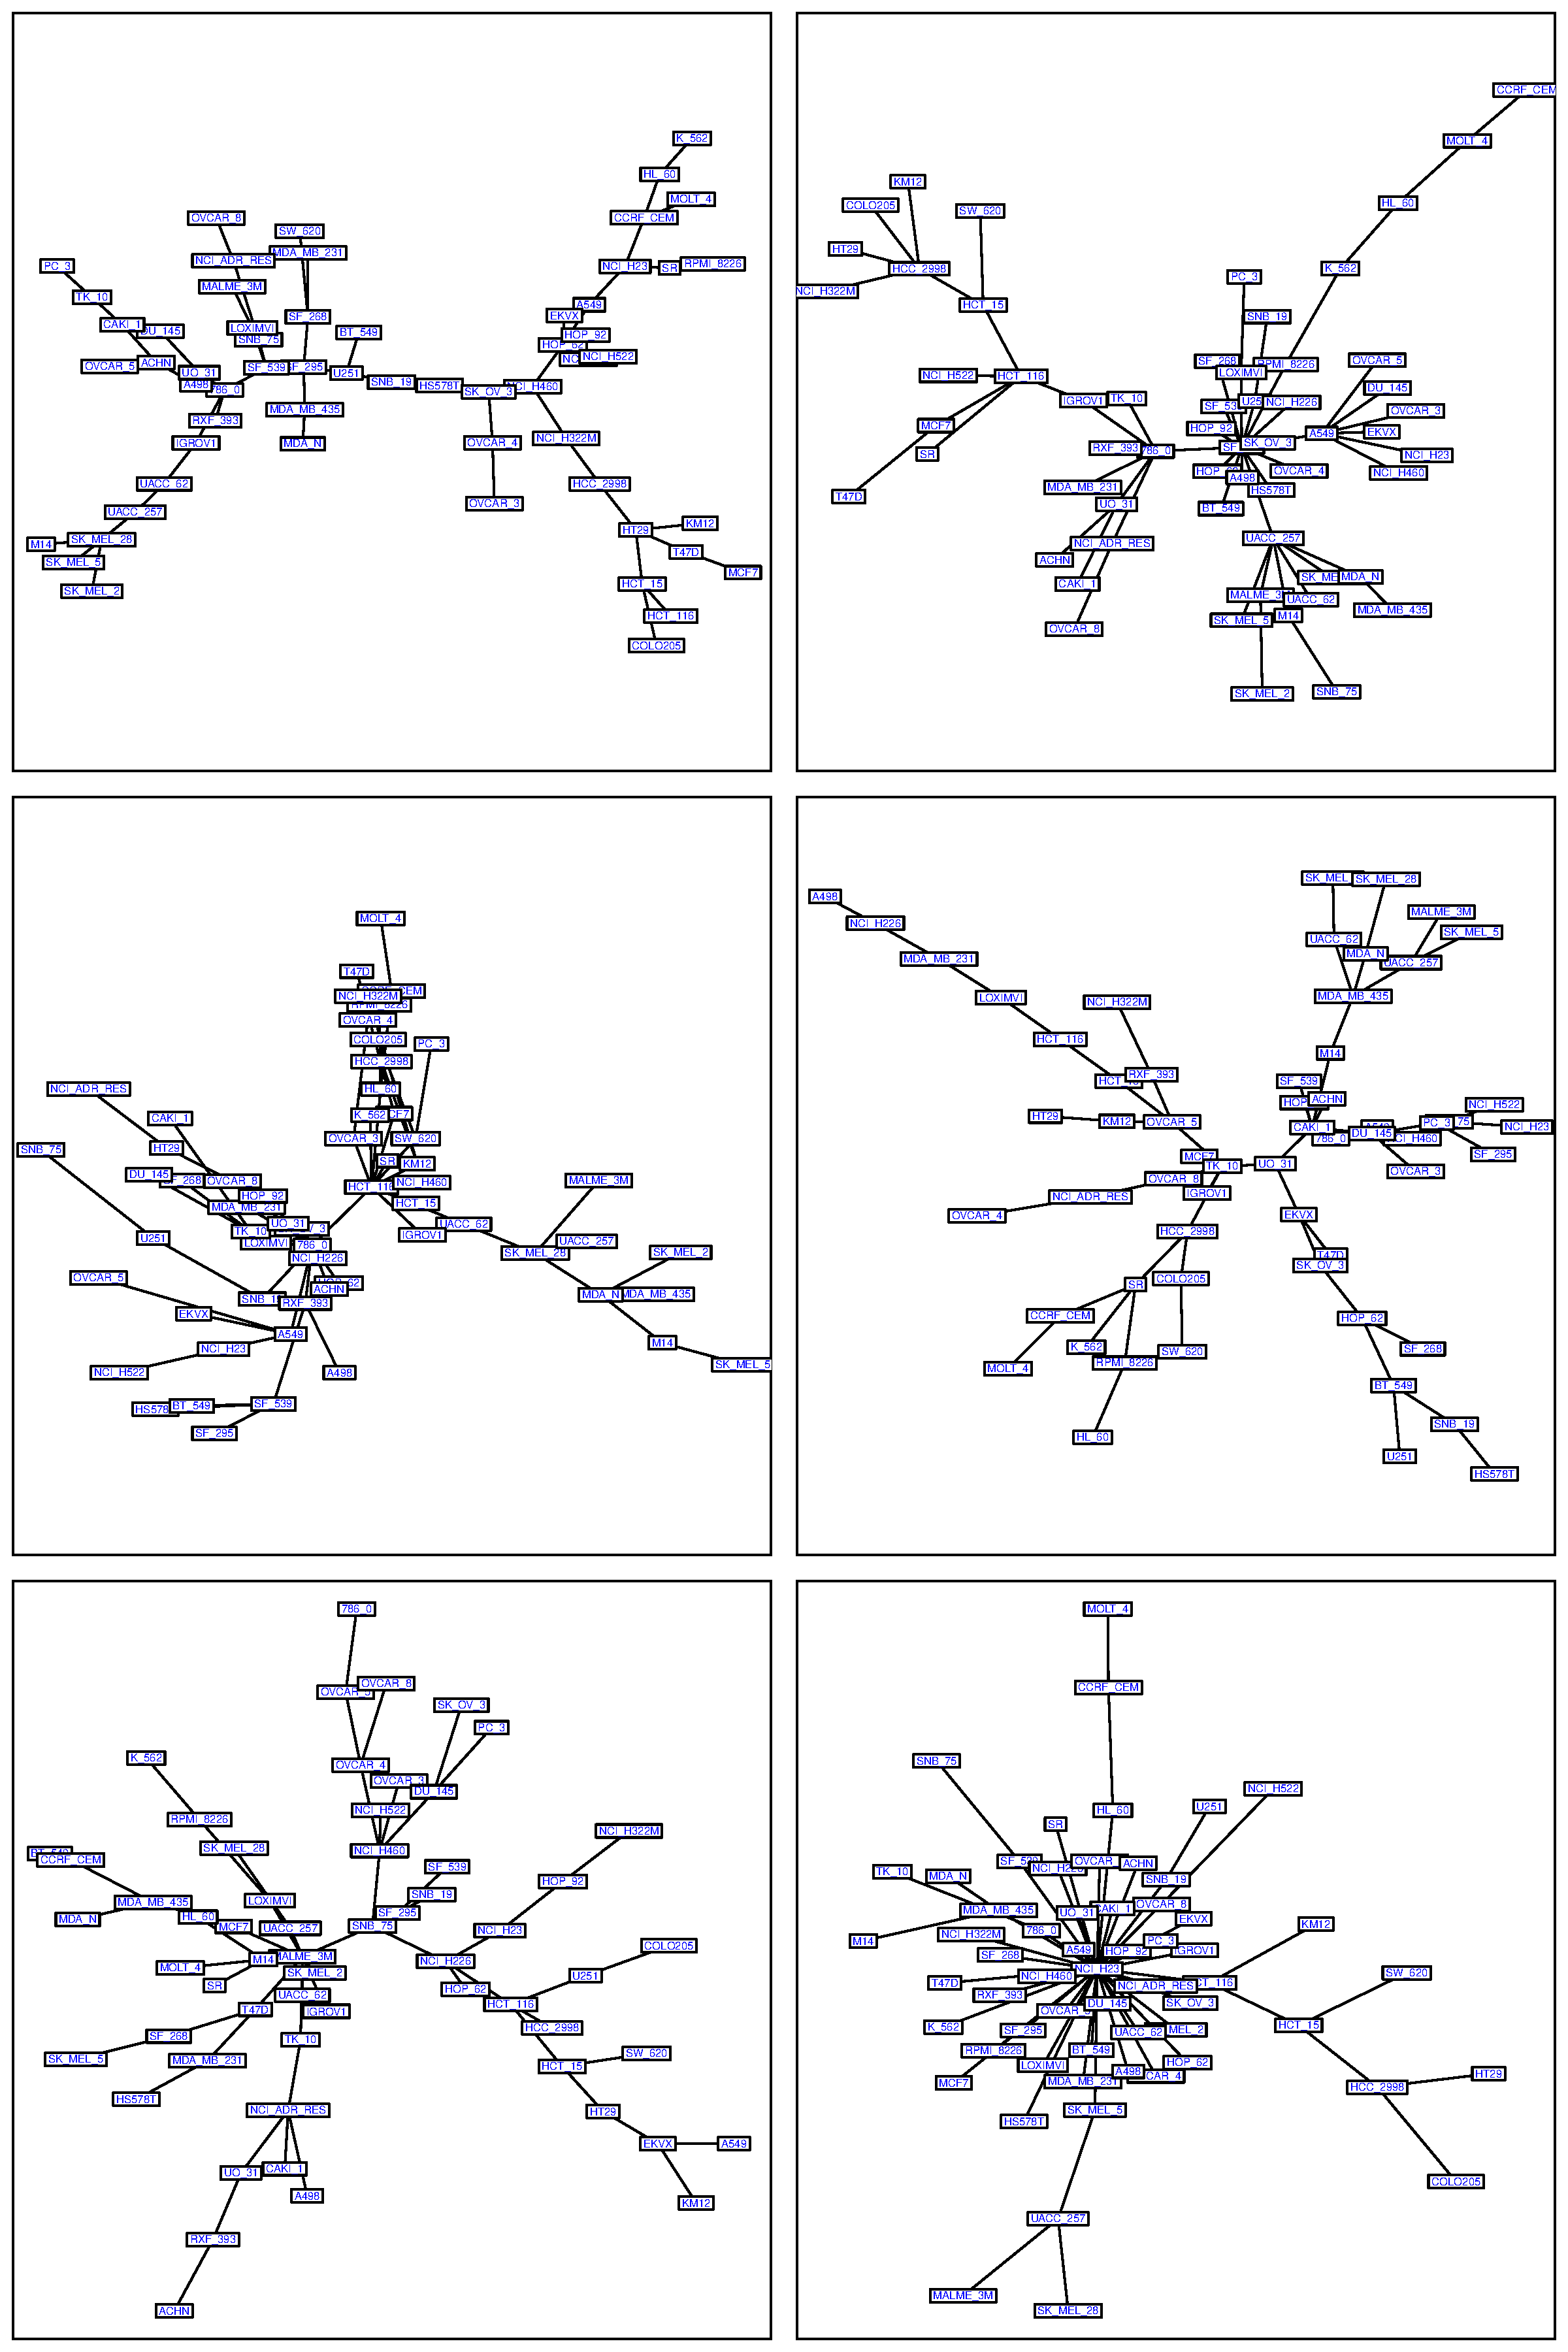
\includegraphics[width=1.0\columnwidth]{./plots/spanning_tree.pdf}
\caption[Spanning trees over cancer cell lines.]{From left to right, top to bottom are spanning tree over cell lines based on reverse-phase lysate arrays, cDNA arrays, Affymetric HU6800 arrays, miRNA arrays, ABC transporter arrays and Affymetric U133 arrays \cite{shankavaram09}.}
\label{spanning_tree}
\end{center}
\end{figure}

\begin{figure}[t]
\begin{center}
\centering
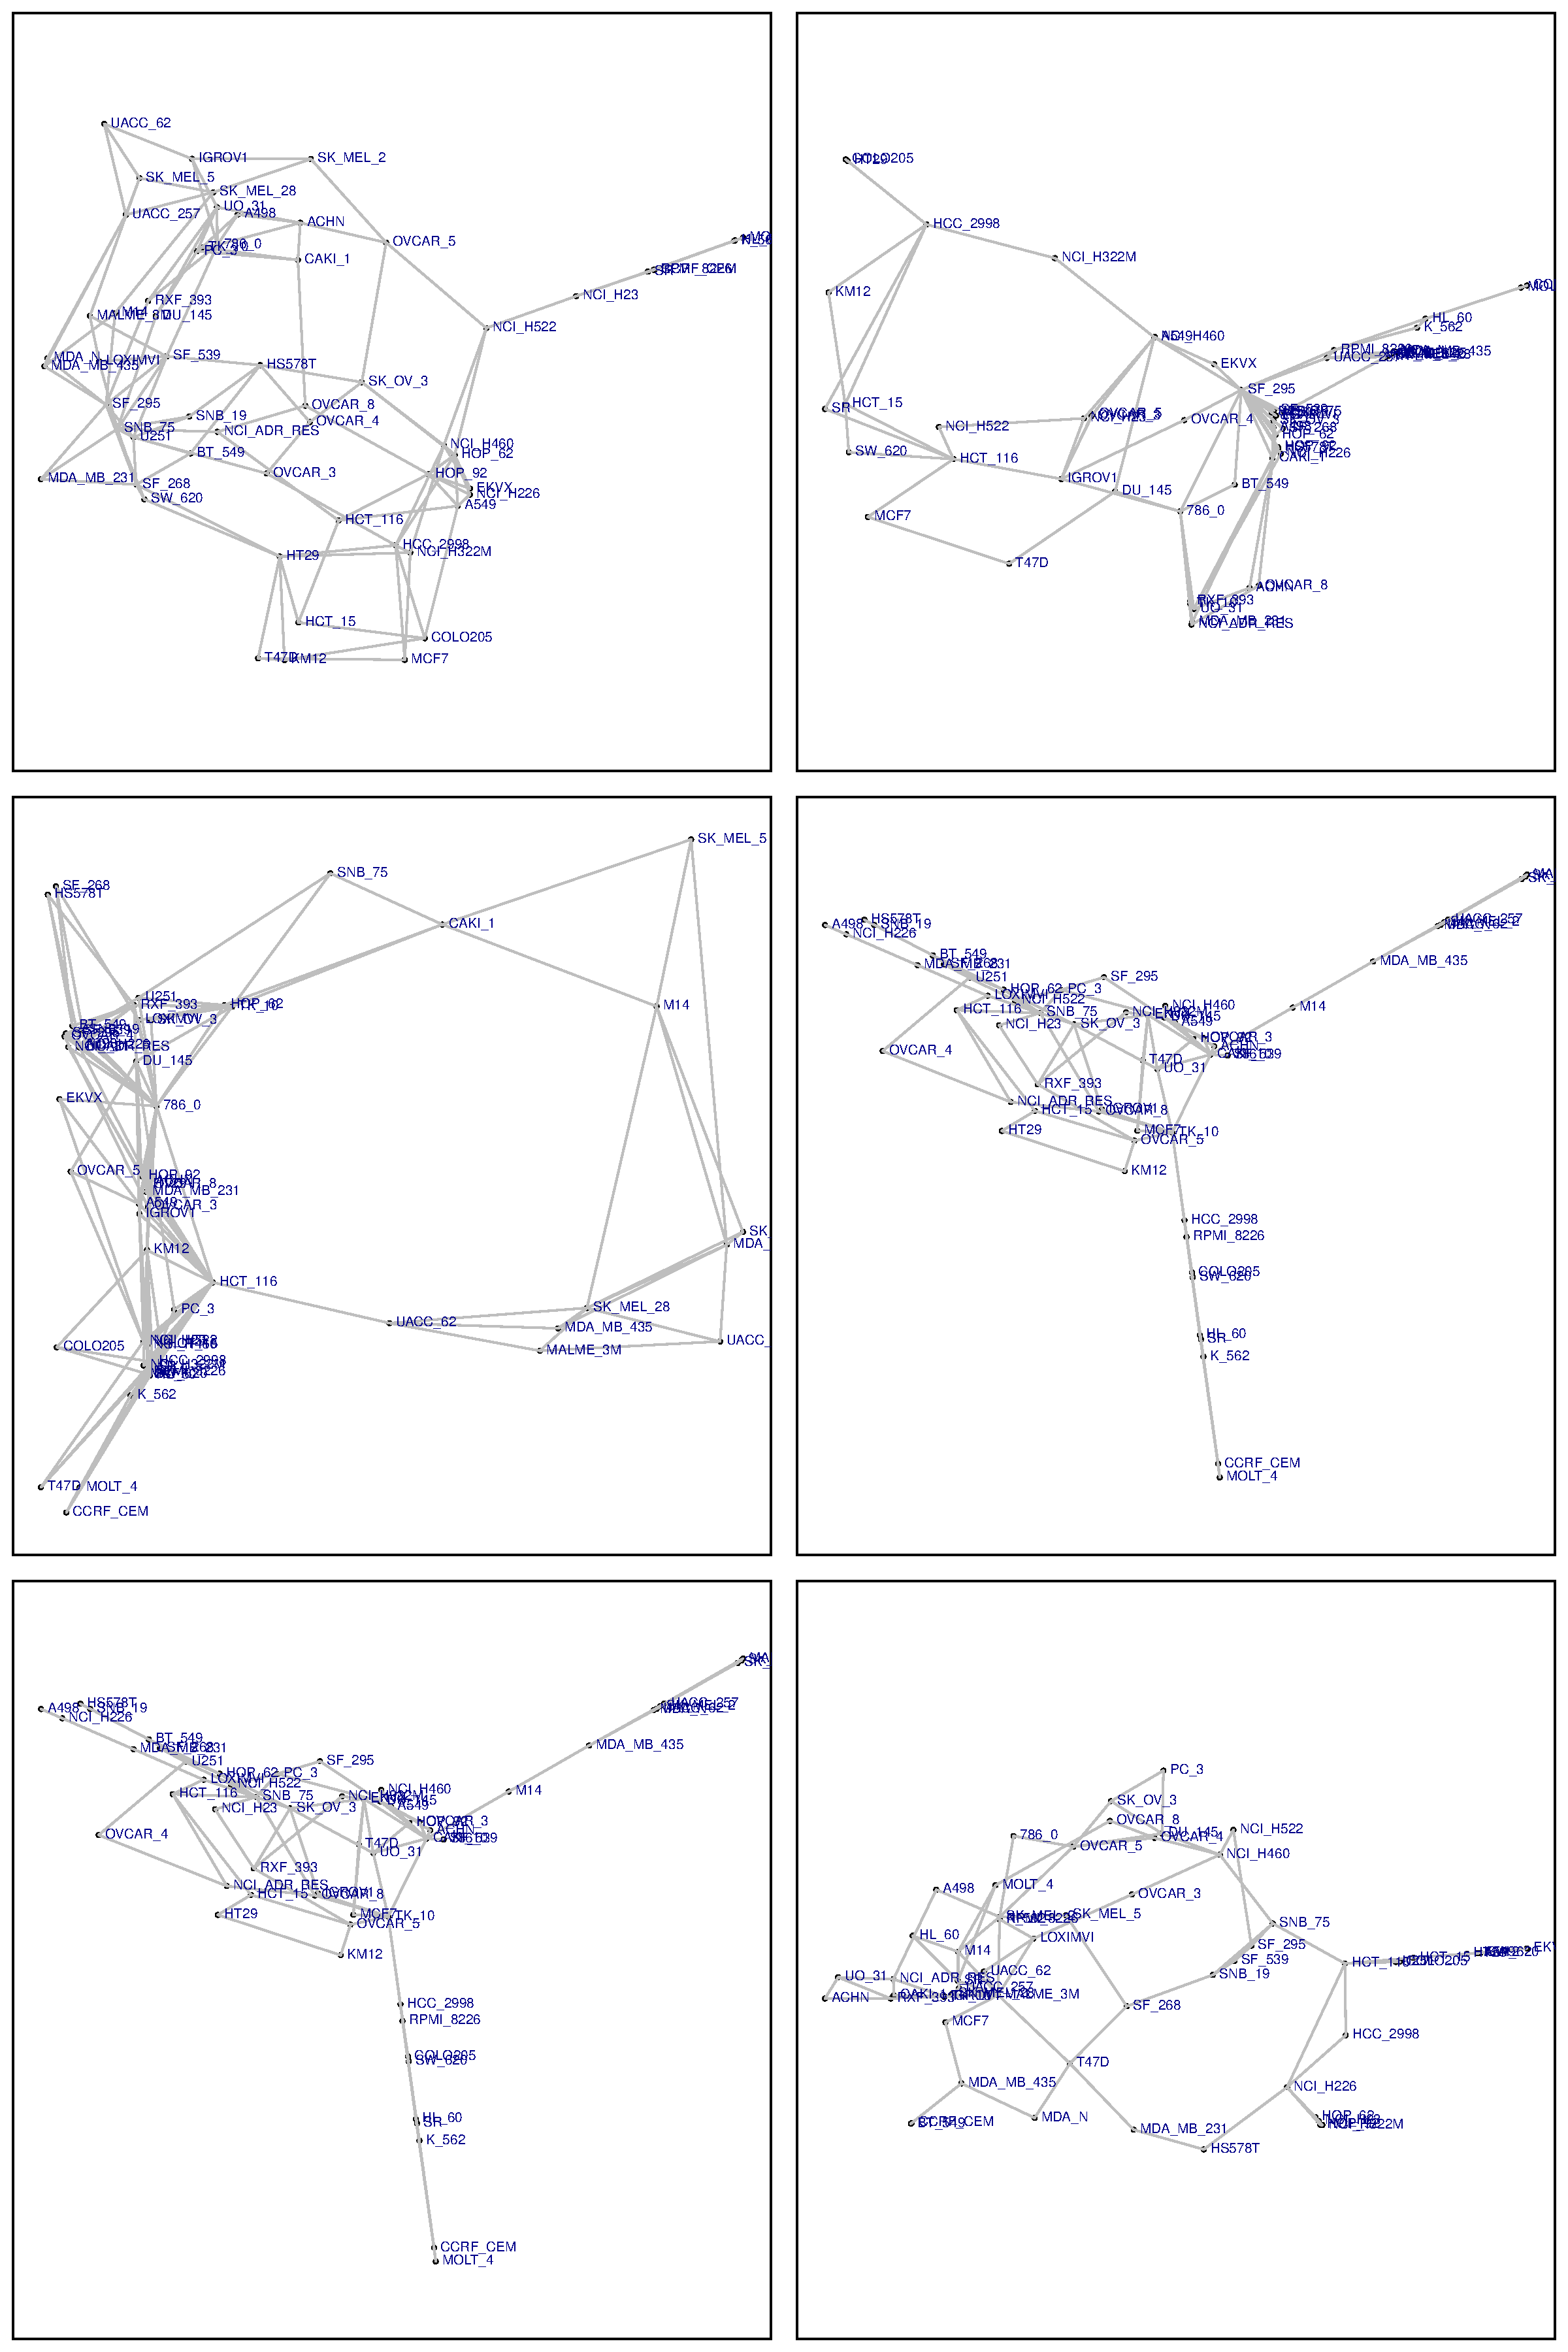
\includegraphics[width=1.0\columnwidth]{./plots/isomap.pdf}
\caption[Markov network from correlation thresholding over cancer cell lines.]{From left to right, top to bottom are Markov network over cell lines by correlation thresholding based on reverse-phase lysate arrays, cDNA arrays, Affymetric HU6800 arrays, miRNA arrays, ABC transporter arrays and Affymetric U133 arrays \cite{shankavaram09}.}
\label{covariance_thresholding}
\end{center}
\end{figure}


\begin{comment}
The notations and descriptions of high throughput experimental data employed in our experiments are illustrated in Table~\ref{auxiliary_data}.


\begin{center}
\begin{table}
\centering
\begin{tabular}{|c|p{3in}|}\hline
\textbf{\em Notation}	&\textbf{\em Description}\\ \hline \hline
Protein & Reverse-phase lysate array for $176$ antibodies. \\ \hline
cDNA & RNA cDNA array of $9,700$ clones with two-color flourescence labeled. \\\hline
HU6800 & High density microarrays (Affymetrix HU6800 chips) with profiling of approximately $6,000$ genes. \\ \hline
miRNA & \\ \hline
Rad & RNA profiles of radiation response in cell lines\\ \hline
Trans & \\ \hline
U133 & Affymetric HG-U133 array with over $1,000,000$\\ \hline

\end{tabular}
\caption{Notation and description of high throughput datasets used as auxiliary data.}
\label{auxiliary_data}
\end{table}
\end{center}
\end{comment}




%%%%%%%%%%%%%%%%%%%%%%%%%%%%%%%%%%%%%%%%%%%%%%%%%%%%%%%%%%%%%%%%%%%%%%%%%%%%%
%
%	Experimental setups, measure of success, and experimental results
%
%%%%%%%%%%%%%%%%%%%%%%%%%%%%%%%%%%%%%%%%%%%%%%%%%%%%%%%%%%%%%%%%%%%%%%%%%%%%%
\clearpage
\section{Experimental results}

We implemented several kernel methods, described in Section~\ref{kernel_methods_sc}, for classification purposes of drug-like molecules. We also built up binary and structural classifiers with MMCRF and SVM algorithms, and tested their performances on several datasets. However, there are numbers of parameters that need to be adjusted before we can actually carry out our experiments. We also need to define the measurements for comparing different classifiers.

In this section, we will first introduce the standards we used in our experiments for evaluation of different classifiers. Then, the choices of kernel parameters and SVM parameters will be briefly discussed. After that, we will focus on binary classification problem in order to find the best classifier on the problem. Finally, we will devote to structural classification problem and demonstrate the improvements we got compared to binary classification. 

\subsection{Measurement of success}

\subsubsection{Statistical measurement}

In order to achieve fair comparisons over different classifiers, we need to define the standards we will use as the measurements of the performances. For a binary classification problem, where data are labeled either {\em positive} or {\em negative}, there are four possible outcomes. If a {positive} example is labeled also as {positive} by the classifier, it is called {\em true positive} (tp). If the predictor gives a {negative} label to an example which is actually {positive}, it is then known as {\em false negative} (fn). Conversely, it is called {\em true negative} (tn) if an actual {negative} example being labeled as {negative}. {\em False positive} (fp) means a {negative} example is labeled as {positive}. The corresponding confusion matrix is defined in Table~\ref{confusion_matrix}. Here, we consider several different statistical measurements to evaluate the behaviors of classifiers:


\begin{description}
\item[Accuracy.] The prediction accuracy ($ACC$) is the ratio of the number of correct predictions (true positive and true negative) against the whole population, defined as
\begin{align*}
ACC = \frac{tp + tn}{tp + fp + tn + fn}.
\end{align*}
Accuracy is suitable for the balanced datasets which have almost equivalent number of positive and negative examples. When datasets are not balanced, the predictions are dominated by ones from bigger classes which leads to a high accuracy but bad classifier performance. Accuracy is bounded between zero and one, where one means all predictions are correct.

\item[Precision and recall.] Precision ($PRE$) is the ratio of true positive predictions against all positive predictions, defined as
\begin{align*}
PRE = \frac{tp}{tp + fp}.
\end{align*}
A precision $PRE = 1$ means all positive prediction are correct (nothing about negative predictions). On the other hand, recall ($REC$) is the ratio of true positive predictions against all real positive examples, defined as
\begin{align*}
REC = \frac{tp}{tp + fn}.
\end{align*}


\item[F1 score.] F1 score ($F_1$) is the weighted average of precision and recall. The commonly used F1 score is defined as
\begin{align*}
F_1 = 2 \cdot \frac{PRE \cdot REC}{PRE + REC},
\end{align*}
where precision and recall are evenly weighted.

\begin{center}
\begin{table}
\centering
\begin{tabular}{|c|c|p{2.4cm}|p{2.4cm}|c|}
\cline{1-5}
\multicolumn{2}{|c|}{} & \multicolumn{2}{|c|}{\textbf{\em Real value}} &\\ \cline{3-4}
\multicolumn{2}{|c|}{} & Positive & Negative &\\ \cline{1-5}
\multicolumn{1}{|c|}{\multirow{2}{*}{\textbf{\em Prediction}}} &
\multicolumn{1}{|c|}{Positive} & {\em true positive} & {\em false positive} & {\em sensitivity}    \\ \cline{2-5}
\multicolumn{1}{|c|}{}                        &
\multicolumn{1}{|c|}{Negative} & {\em false negative} & {\em true negative}  & {\em specificity}  \\ \cline{1-5}
%\multicolumn{2}{|c|}{} & {\em precision} & {\em recall} &\\ \cline{1-5}
\end{tabular}
\caption[Prediction confusion matrix.]{Prediction confusion matrix.}
\label{confusion_matrix}
\end{table}
\end{center} 

\item[True positive rate and true negative rate.] True positive rate ({\em TPR}) or {\em sensitivity} is the proportion of true positive predictions against all positive examples, which is the same as recall.
\begin{comment}
\begin{align*}
TPR = \frac{tp}{tp + fn}.
\end{align*}
\end{comment}
Similarly, true negative rate ({\em TNR}) or {\em specificity} is the proportion of negative prediction against all negative examples, defined as
\begin{align*}
TNR = \frac{tn}{tn + fp}.
\end{align*}

\item[ROC curve and AUC score.] A receiver operating characteristic ($ROC$) curve is the plot of true positive rate against true negative rate. AUC score ($AUC$) is the area below ROC curve, which is equivalent to the probability that the classifier give a higher score to a randomly picked positive example than to a negative one. AUC score is most often used in machine learning since it also tolerances the unbalanced datasets. A random classifier will have $AUC = 0.5$, and a perfect classifier corresponds to $AUC = 1$.

\item[Two tailed sign test.] In statistics, the two tailed sign test can be used to test the hypothesis that there is no significant differences for two random variables, when we randomly draw pair of examples from them. The hypothesis will be rejected if the value of the statistics is either sufficiently small or sufficiently large. 

\end{description}



\subsubsection{Validation methods}

In machine learning, the statistical measurements are usually reported from a {\em $k$-fold cross validation} procedure. In a $k$-fold cross validation, the dataset is randomly divided into $k$ subsets. Each subset is served as validation dataset for testing the classifier, and the rest $k-1$ subsets are served as training data for learning a classifier at the same time. This is repeated $k$ times, until each subset is used exactly once as a training set. The cross validation procedure ensure there is no bias generated during learning phrase. 

The {\em leave-one-out cross validation} is a special version of $k$-fold cross validation. It uses each single example as testing data and the rest of examples as training data, until all examples in the dataset are tested once. It is a validation method that commonly used for small datasets. Therefore the statistical measurements on Mutag dataset are reported from a leave-one-out cross validation procedure.

NCI-cancer dataset is high biased in the sense that molecules are not well distributed according to the number of cell lines they are active against, as shown in Figure~\ref{activity_hist}. Therefore, we adopted a stratified $5$-fold cross validation procedure on NCI-cancer dataset. We arrange molecules into $60$ groups according to the number of cell lines they are active against, and divide molecules of each group into $5$ subsets. In each iteration, we use one subset from each group as validation data and the rest of the subsets as training data. It is then repeated five times, until all data are taken once as testing examples. Therefore, we further address the skewness of the cancer dataset.


\subsection{Experimental setup}
\label{experimental_setup}

We used graph representation for molecules in our experiments. Hydrogen atoms are excluded in our graph representations. MOL2 files are also employed to improve the performances of the classifiers. We did not use reduced graph representation. However, it is still quite an interesting approach, and we will explore it in the future work.

Kernel parameters corresponds to the set of features we put into consideration. Therefore, they are very important  in our experiments. We focus on walk kernel with walks of finite length, and calculate it in a dynamic programming fashion. Since optimized parameters for finite length walk kernel was not mentioned in any publications, we explicitly test the parameters of walk kernel on Mutag dataset, and keep the optimized parameter in later experiments. The maximum length of the walk is decided by parameter $l$, with the range of $(1 \le l \le 11)$ in our experiments. The down scaling parameter $\lambda$ of walk kernel takes the value from $0.01$ to $0.11$  with a step of $0.01$. For the weighted decomposition kernel, we use the version with neighbors of contextor radius three and atom type property only, as recommended in \cite{ceroni07}. Hash fragment features are extracted explicitly for all fragments of length $6$, which is the default value in Openbabel. Functional group features also follow the functional group definition in OpenBabel. No additional parameters were needed for Tanimoto kernel. All kernels are normalized. For the following experiments, we use notations for different kernel methods other than their full names. Notations are described in Table~\ref{kernel_notation}.

We used the SVM implementation of the libSVM software package written in C++\footnote{http://www.csie.ntu.edu.tw/~cjlin/libsvm/}. We tested various values of $C$ ranging from one to 100. Relative hard margin $(C=100)$ emerged as the value we used in subsequent experiments. We used $\xi = 0.01$ in our experiments.

\begin{center}
\begin{table}
\centering
\begin{tabular}{|c||p{5.8cm}|}\hline
%\textbf{\em Cell line}	&\textbf{\em Active}	&\textbf{\em Inactive}	&\textbf{\em Active \%}	&\textbf{\em Cell line}	&\textbf{\em Active}	&\textbf{\em Inactive} &\textbf{\em Active \%}	\\ \hline \hline
\textbf{\em Notation}	&\textbf{\em Kernel method}\\ \hline \hline
WK & Walk kernel with finite length of walks \\ \hline
WDK & Weighted decomposition kernel \\ \hline
HF & Hash fragment features \\ \hline
SK & Substructure key features \\ \hline
TK & Tanimoto kernel \\ \hline
\end{tabular}
\caption[Notations for different kernel methods.]{Notations for different kernel methods.}
\label{kernel_notation}
\end{table}
\end{center}


\subsection{Binary classification}

\subsubsection{Mutag dataset}

With the basic experimental designs, we first tried to optimize walk kernel parameters $l$ and $\lambda$ on Mutag dataset. In the first experiment, we constructed walk kernel on Mutag dataset with fixed $l=10$ and various $\lambda$ parameters that took values from $0.01$ to $0.11$ with a step of $0.01$. SVM parameter $C$ was fixed on $C=100$. We report in Figure~\ref{result_mutag_lambda} the accuracies, AUC scores and F1 scores of different $\lambda$ from a leave-one-out cross validation. The optimized $\lambda$ parameter for walk kernel is $0.11$, which can be seen from the results. 

Then, we fix $\lambda = 0.11$, and tested the effect of $l$ parameter. We took different $l$ parameters ranging from $1$ to $10$. The accuracies, AUC scores and F1 scores are reported in Figure~\ref{result_mutag_l}. As demonstrated in the results, different $l$ lead to almost the same performance, while $l = 5$ gives the best results. Therefore, the parameters for walk kernel were set to $\lambda = 0.11$ and $l=5$, which achieve the accuracy of $81.38\%$, AUC score of $87.05\%$ and F1 score of $85.71\%$. The classification accuracy and AUC score match the state-of-the-art performance on Mutag dataset described in \cite{mahe04}.

\begin{figure}[t]
\begin{center}
\centering
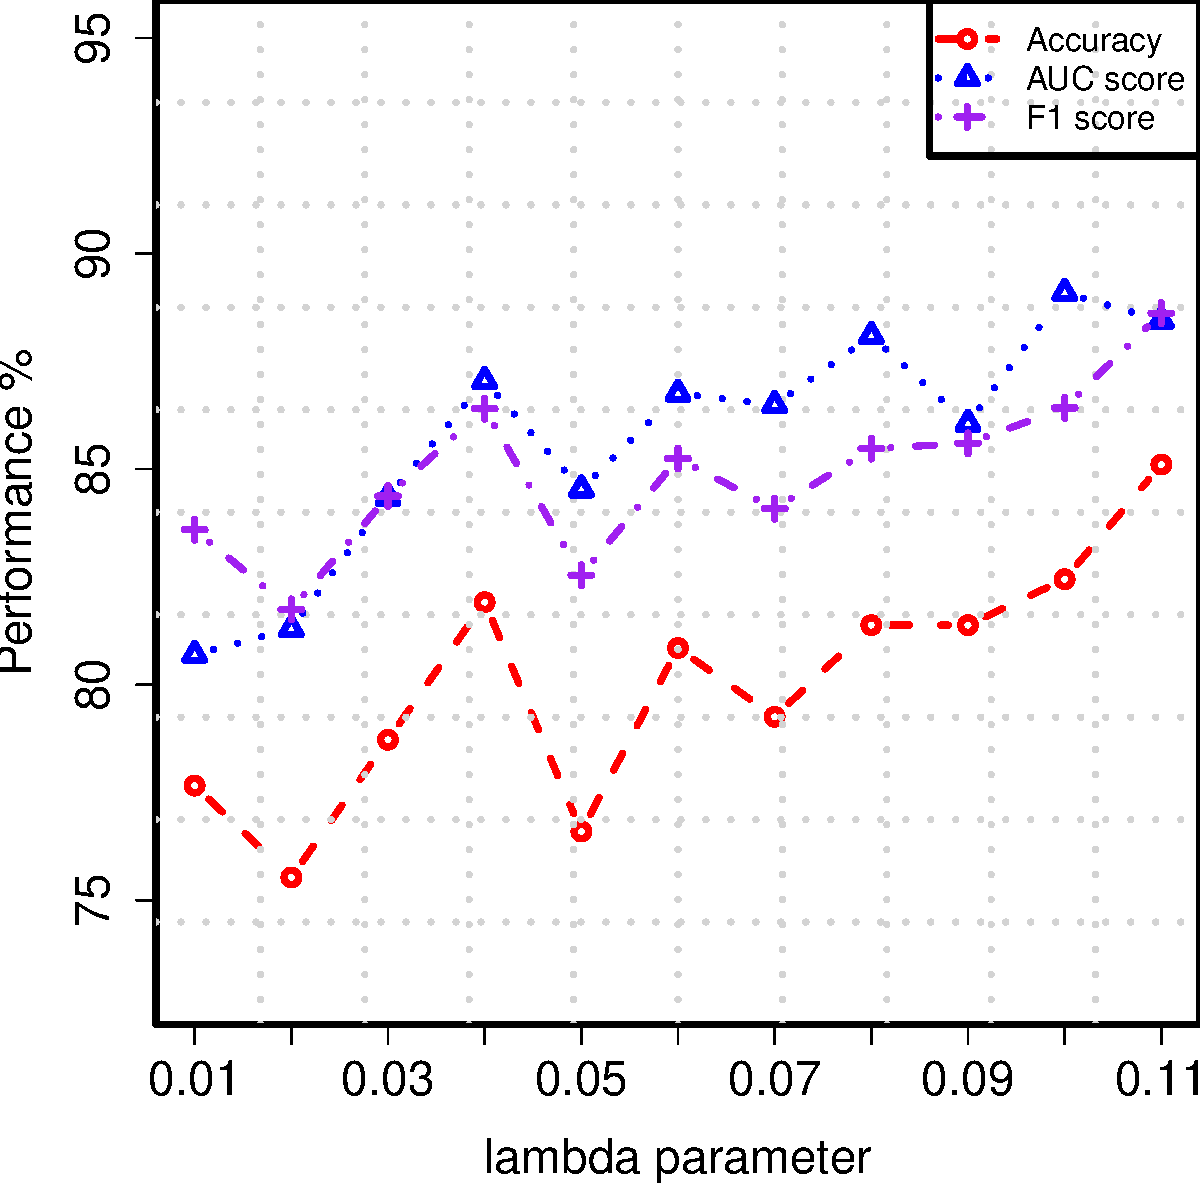
\includegraphics[width=0.6\columnwidth]{./plots/result_mutag_lambda.pdf}
\caption[Parameter $\lambda$ of walk kernel.]{Parameter $\lambda$ of walk kernel on Mutag dataset.}
\label{result_mutag_lambda}
\end{center}
\end{figure}

\begin{figure}[t]
\begin{center}
\centering
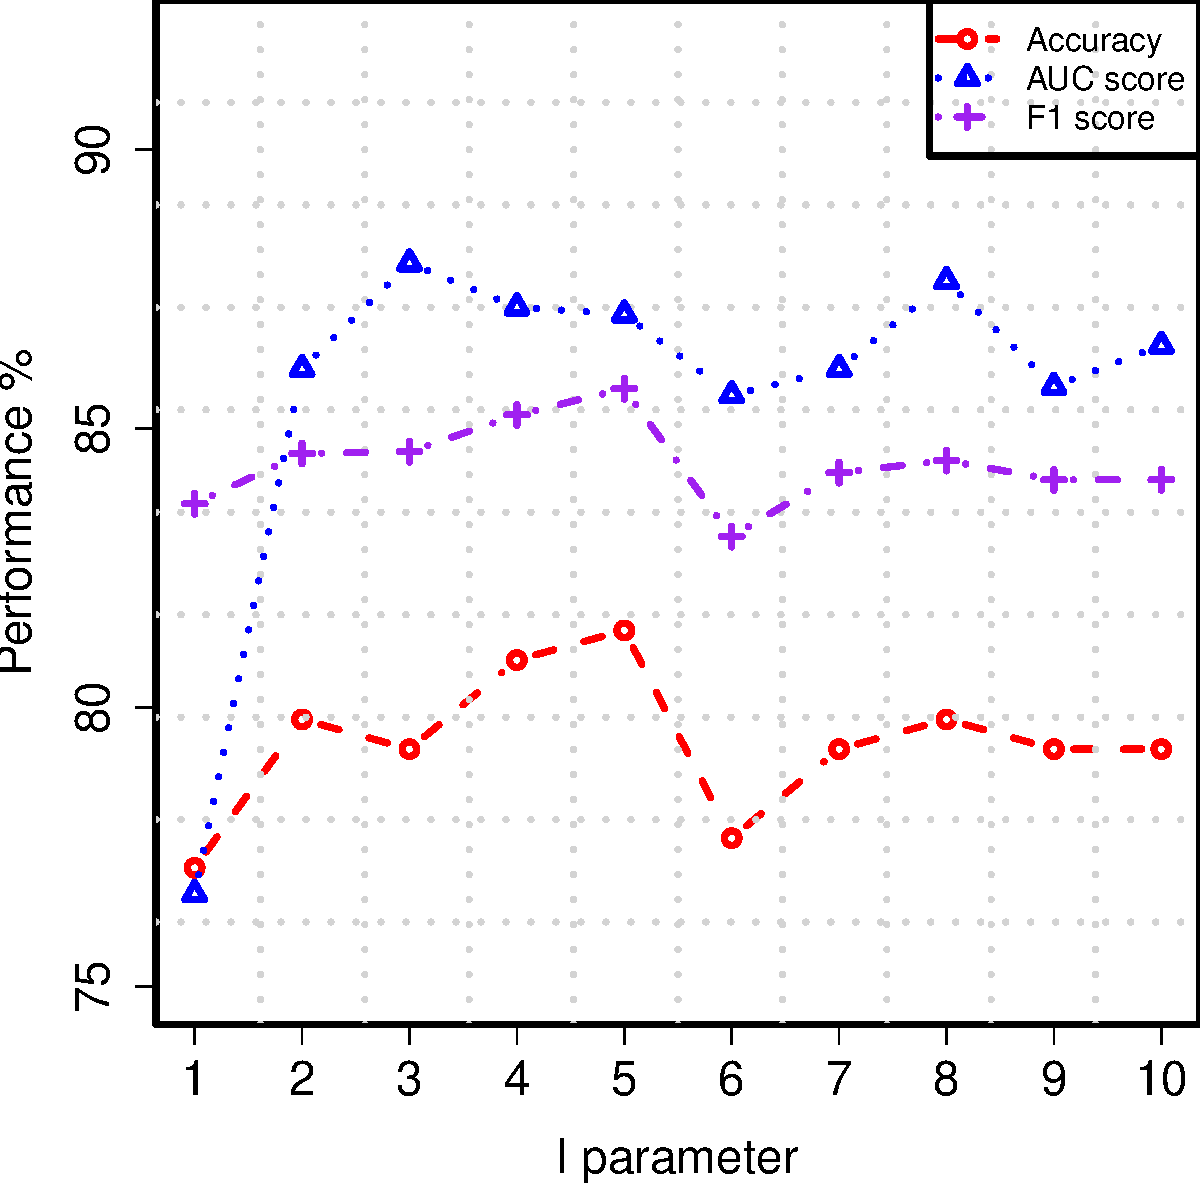
\includegraphics[width=0.6\columnwidth]{./plots/result_mutag_l.pdf}
\caption[Parameter $l$ of walk kernel.]{Parameter $l$ of walk kernel on Mutag dataset. $\lambda$ is set to $0.11$.}
\label{result_mutag_l}
\end{center}
\end{figure}

Next, we considered other kernel methods mentioned in Table~\ref{kernel_notation}. We explicitly constructed these kernels on Mutag dataset, where walk kernel took the parameter settings from the previous experiments and parameters of other kernels followed the description in Section~\ref{experimental_setup}. We report classification accuracies, AUC scores and F1 scores in Table~\ref{result_mutag_all}. 

Overall, the best kernel methods that works on Mutag dataset is Tanimoto kernel (TK) with hash fragments features (HF), which achieves the best accuracy, AUC score and F1 score in our experiments. Tanimoto kernel with functional group features behaves similarly to the one with hash fragment features. While, walk kernel and weighted decomposition kernel are almost equivalent and are not as good as the Tanimoto kernel.

\begin{center}
\begin{table}
\centering
\begin{tabular}{|c||c|c|c|}\hline
\textbf{\em Classifier}	&\textbf{\em Accuracy } &\textbf{\em AUC score } &\textbf{\em F1 score }\\ \hline \hline
TK+HF & \textbf{86.17\%} & \textbf{89.94\%} & \textbf{89.76\%} \\ \hline
TK+FG & 84.57\% & 86.57\% & 88.63\% \\ \hline
WDK & 81.38\% & {89.18\%} & 86.06\% \\ \hline
WK & 81.38\% & 87.05\% & 85.71\% \\ \hline
\end{tabular}
\caption[Classifier performances on Mutag dataset.]{Performances of classifiers on Mutag dataset.}
\label{result_mutag_all}
\end{table}
\end{center}



\subsubsection{NCI-cancer dataset}

We continued to test the behaviors of different kernel methods on binary classification of NCI-cancer dataset. We have prepared three versions of NCI-cancer dataset, as proposed in Section~\ref{NCI_cancer_datasets}. Kernels were explicitly constructed, where walk kernel took the optimized parameter from previous section and parameters of other kernels followed the setting illustrated in Section~\ref{experimental_setup}.

In the first experiment, we used the version of NCI-cancer dataset which includes only the middle-active molecules. We report average accuracy, precision, recall and the F1 score of cell lines from different classifiers in Table~\ref{ncicancer_1}\footnote{NA values are generated in precisions and corresponding F1 scores of some cell lines from WDK classifiers. The average precision and F1 scores of WDK are calculated after removing all NA values.}. Tanimoto kernel (TK) with hash fragment features (HF) and functional group features (FG) achieve the competitive results and slightly outperform walk kernel (WK) and weighted decomposition kernel (WDK). 

\begin{center}
\begin{table}
\centering
\begin{tabular}{|c||c|c|c|c|}\hline
\textbf{\em Classifier}	&\textbf{\em Accuracy } &\textbf{\em PRE } &\textbf{\em REC } &\textbf{\em F1 score } \\ \hline \hline
TK+HF & {64.13\%} & {57.45\%} & {50.25\%} & {52.74\%}\\ \hline
TK+FG & 62.55\% & 54.52\% & \textbf{54.31\%} & \textbf{54.06\%} \\ \hline
WDK & 63.86\% & 56.83\% & 49.73\% & 51.64\% \\ \hline
WK & \textbf{64.31\%} & \textbf{58.00\%} & 46.20\% & 47.67\% \\ \hline
\end{tabular}
\caption[Classifier performances on NCI-cancer dataset 1.]{Performance of classifiers on NCI-cancer dataset with middle-active molecules.}
\label{ncicancer_1}
\end{table}
\end{center}

\begin{center}
\begin{table}
\centering
\begin{tabular}{|c||c|c|c|c|}\hline
\textbf{\em Classifier}	&\textbf{\em Accuracy } &\textbf{\em PRE } &\textbf{\em REC } &\textbf{\em F1 score } \\ \hline \hline
TK+HF & \textbf{72.00\%} & \textbf{68.86\%} & \textbf{60.71\%} & \textbf{64.86\%}\\ \hline
TK+FG & 69.61\% & 66.45\% & {58.20\%} & {61.99\%} \\ \hline
WDK & 61.05\% & 55.37\% & 36.19\% & 42.91\% \\ \hline
WK & 62.23\% & 57.38\% & 39.38\% & 45.86\% \\ \hline
\end{tabular}
\caption[Classifier performances on NCI-cancer dataset 2.]{Performance of classifiers on NCI-cancer dataset with no-zero-active molecules.}
\label{ncicancer_2}
\end{table}
\end{center}

\begin{center}
\begin{table}
\centering
\begin{tabular}{|c||c|c|c|c|}\hline
\textbf{\em Classifier}	&\textbf{\em Accuracy } &\textbf{\em PRE } &\textbf{\em REC } &\textbf{\em F1 score } \\ \hline \hline
TK+HF & \textbf{80.34\%} & \textbf{73.41\%} & \textbf{51.99\%} & \textbf{60.73\%}\\ \hline
TK+FG & 79.63\% & 72.19\% & {49.32\%} & {58.48\%} \\ \hline
WDK & 69.46\% & 36.88\% & 7.10\% & 11.57\% \\ \hline
WK & 70.12\% & 43.85\% & 8.67\% & 13.99\% \\ \hline
\end{tabular}
\caption[Classifier performances on NCI-cancer dataset 3.]{Performance of classifiers on NCI-cancer dataset with full data.}
\label{ncicancer_3}
\end{table}
\end{center}

In the second experiment, we used NCI-cancer dataset without zero-active molecules. Table~\ref{ncicancer_2} shows the average accuracies, precisions, recalls and F1 scores from the experiments, where Tanimoto kernel with hash fragment features outperformed other kernel methods. In the following experiments, we uses the dataset with all molecular data which results in similar results, as shown in Table~\ref{ncicancer_3}.


% summary for binary classification

Overall from our experiments on binary classification problem, Tanimoto kernel with hash fragment features outperformed other kernel methods in almost all statistical measurements over all versions of our datasets. It should be noticed that SVM $C$ parameter was set with $C=100$ in all of our experiments in order to achieve fair comparisons of various kernel methods. Increasing $C$, which corresponds to expanding the margin, sometimes improve the performance of the classifiers. 

It is shown that applying polynomial kernel or Gaussian kernel over current kernels will also improve their F1 scores \cite{astikainen08}. Polynomial kernel was also employed as a standard setting for kernel methods in \cite{menchetti05, ceroni07}. However, we did not use any polynomial or Gaussian kernel recomposition since we only wanted to compare different kernel methods.




%%%%%%%%%%%%%%%%%%%%%%%%%%%%%%%%%%%%%%%%%%%%%%%%%%%%%%%%%%
\subsection{Multilabel structural classification}

Compared to binary classification which predicts a single label at a time, multilabel structural classification manages to predict all labels in one shot. The classifier also includes information on dependencies among single labels represented as the structure. In this section, we will focus on multilabel structural classification, and make the comparisons against binary classifiers constructed by SVM. The NCI-cancer dataset, which is a multilabeled dataset, will be employed in the experiments. Since Tanimoto kernel with hash fragments features was proved to be the best kernel from binary classification experiments, we will also used it to construct MMCRF classifiers.

\subsubsection{Effect of Markov network}
% TODO
We report in Figure~\ref{graph_effect} the prediction accuracies on dataset with middle-active molecules using various Markov networks, as describe in Section~\ref{markov_network_sc}. The prediction accuracies on different Markov network structures differ slightly. The best accuracy was given by using maximum weighted spanning tree approach on RNA radiation array dataset, shown in Figure~\ref{net}, which describes profiles of radiation response in cell lines. This meets our expectations since cancer cells mostly mutated from normal cells and normal cells with radiation treatments can possibly explain the mutations.

We also used random graphs over cell lines. However, predictions based on random Markov networks were not able to give as good results as the ones constructed from auxiliary data.

\begin{figure}[t]
\begin{center}
\centering
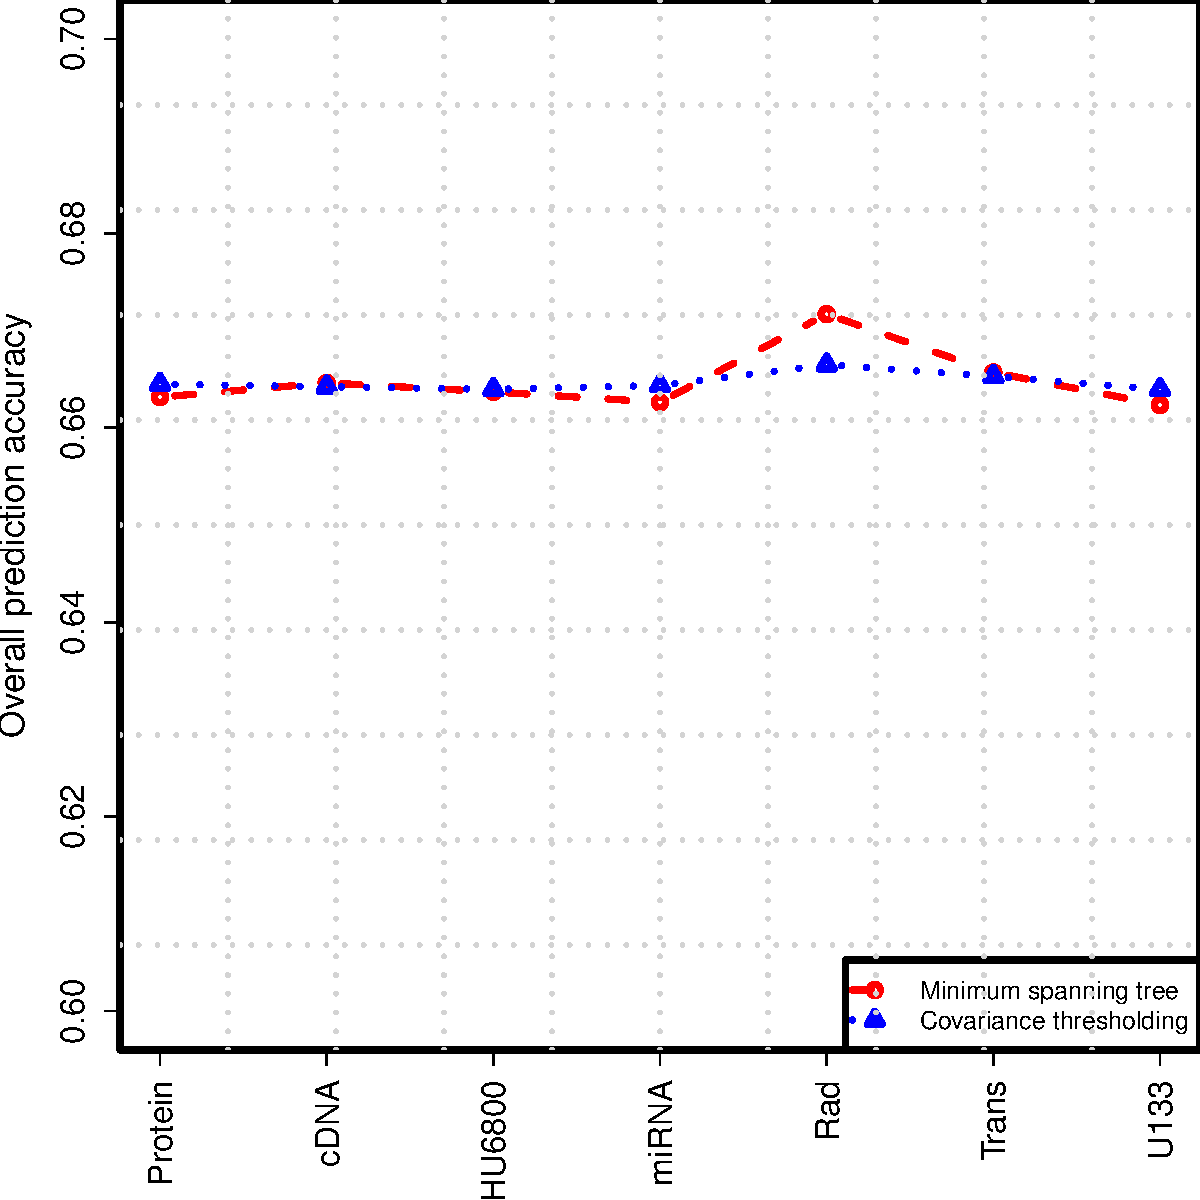
\includegraphics[width=0.65\columnwidth]{./plots/graph_effect.pdf}
\caption[Effects on Markov network in MMCRF.]{Effects of Markov network construction methods and type of auxiliary data (from left to right: reverse-phase lysate arrays, cDNA arrays, Affymetric HU6800 arrays, miRNA arrays, RNA radiation arrays, ABC transporter arrays, and Affymetrix U133 arrays). }
\label{graph_effect}
\end{center}
\end{figure}

\begin{figure}[h]
\begin{center}
\centering
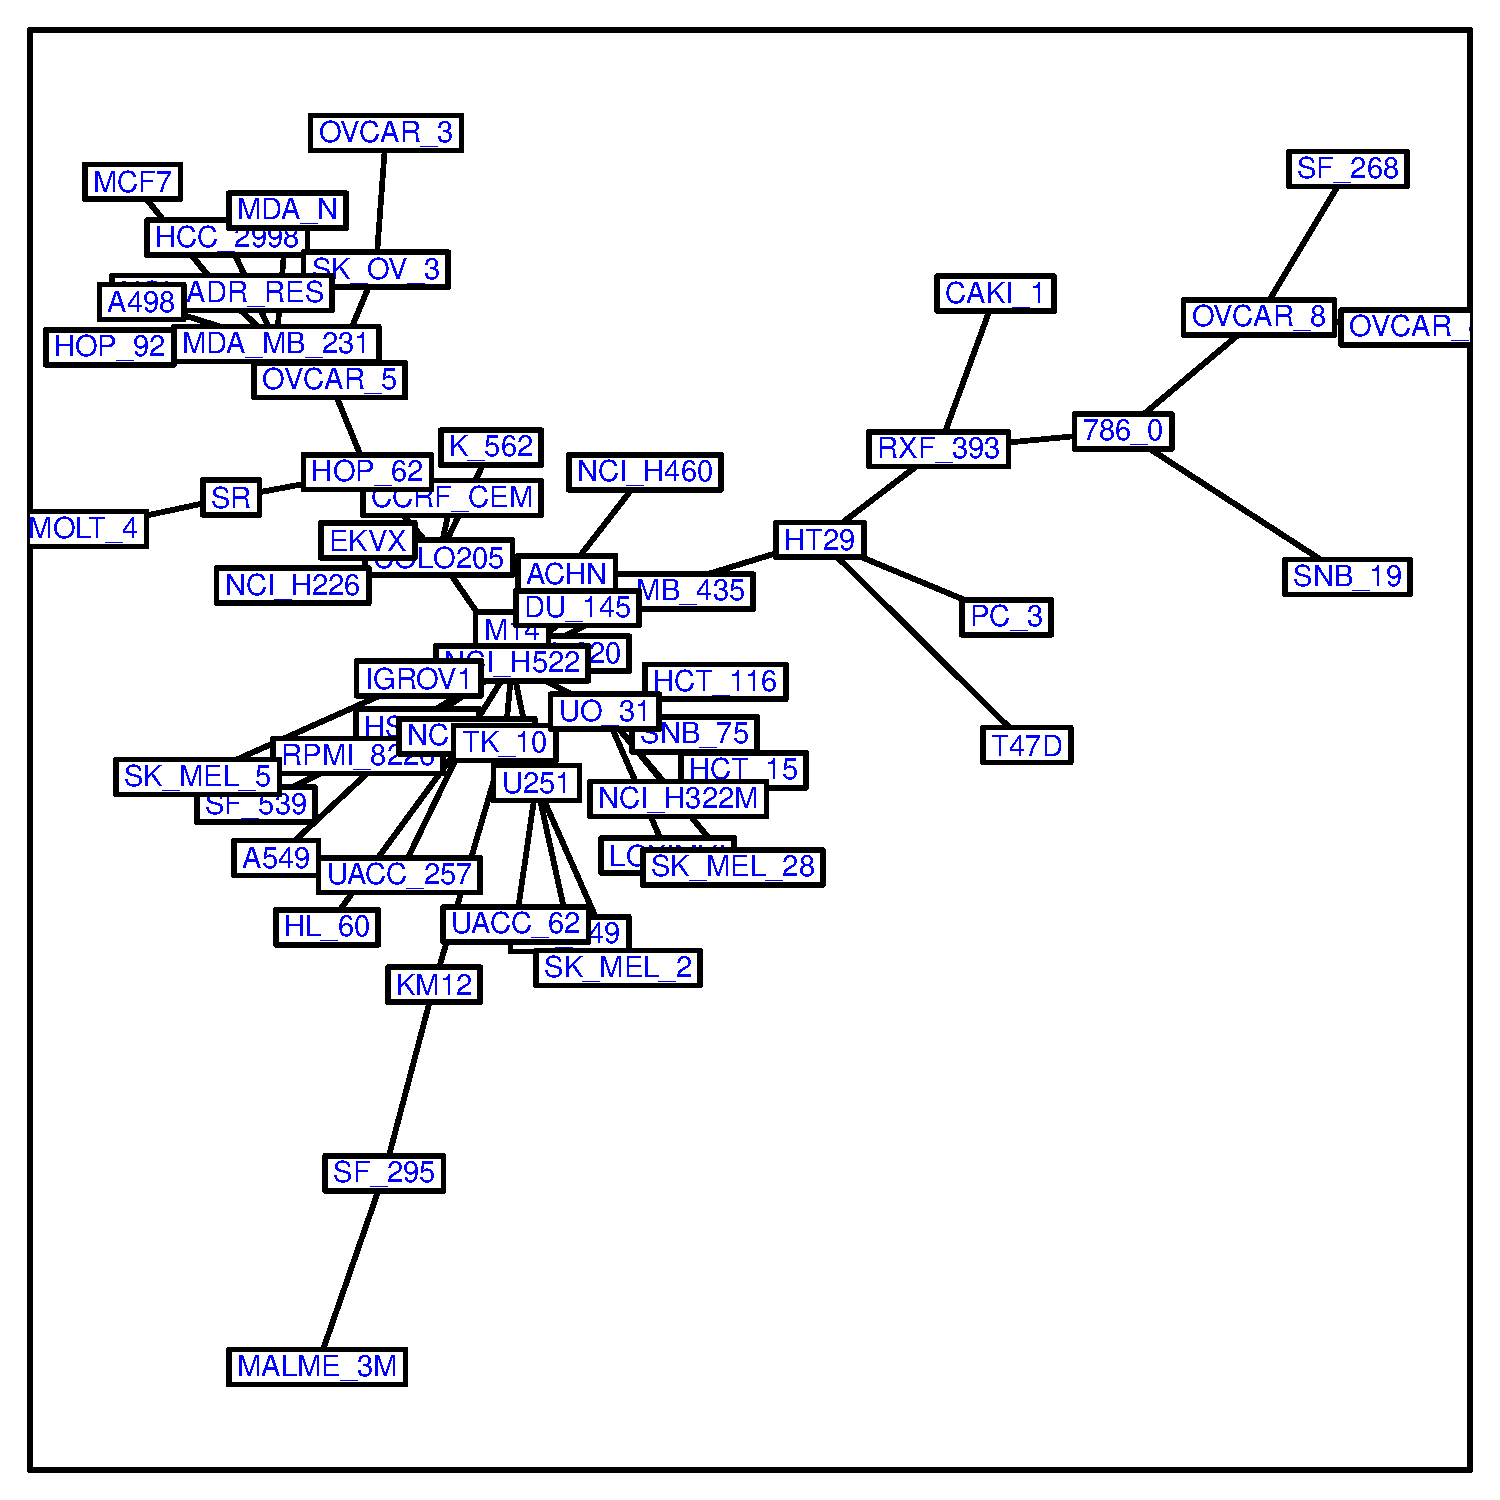
\includegraphics[width=0.65\columnwidth]{./plots/net.pdf}
\caption[Spanning tree from RNA radiation array.]{Markov network constructed from maximum weighted spanning tree method on RNA radiation array data \cite{shankavaram09}. The labels correspond to different cancer cell lines.}
\label{net}
\end{center}
\end{figure}


\subsubsection{Effect of dataset version}

%TODO overall accuracies and F1 scores from SVM and MMCRF
\begin{figure}[p]
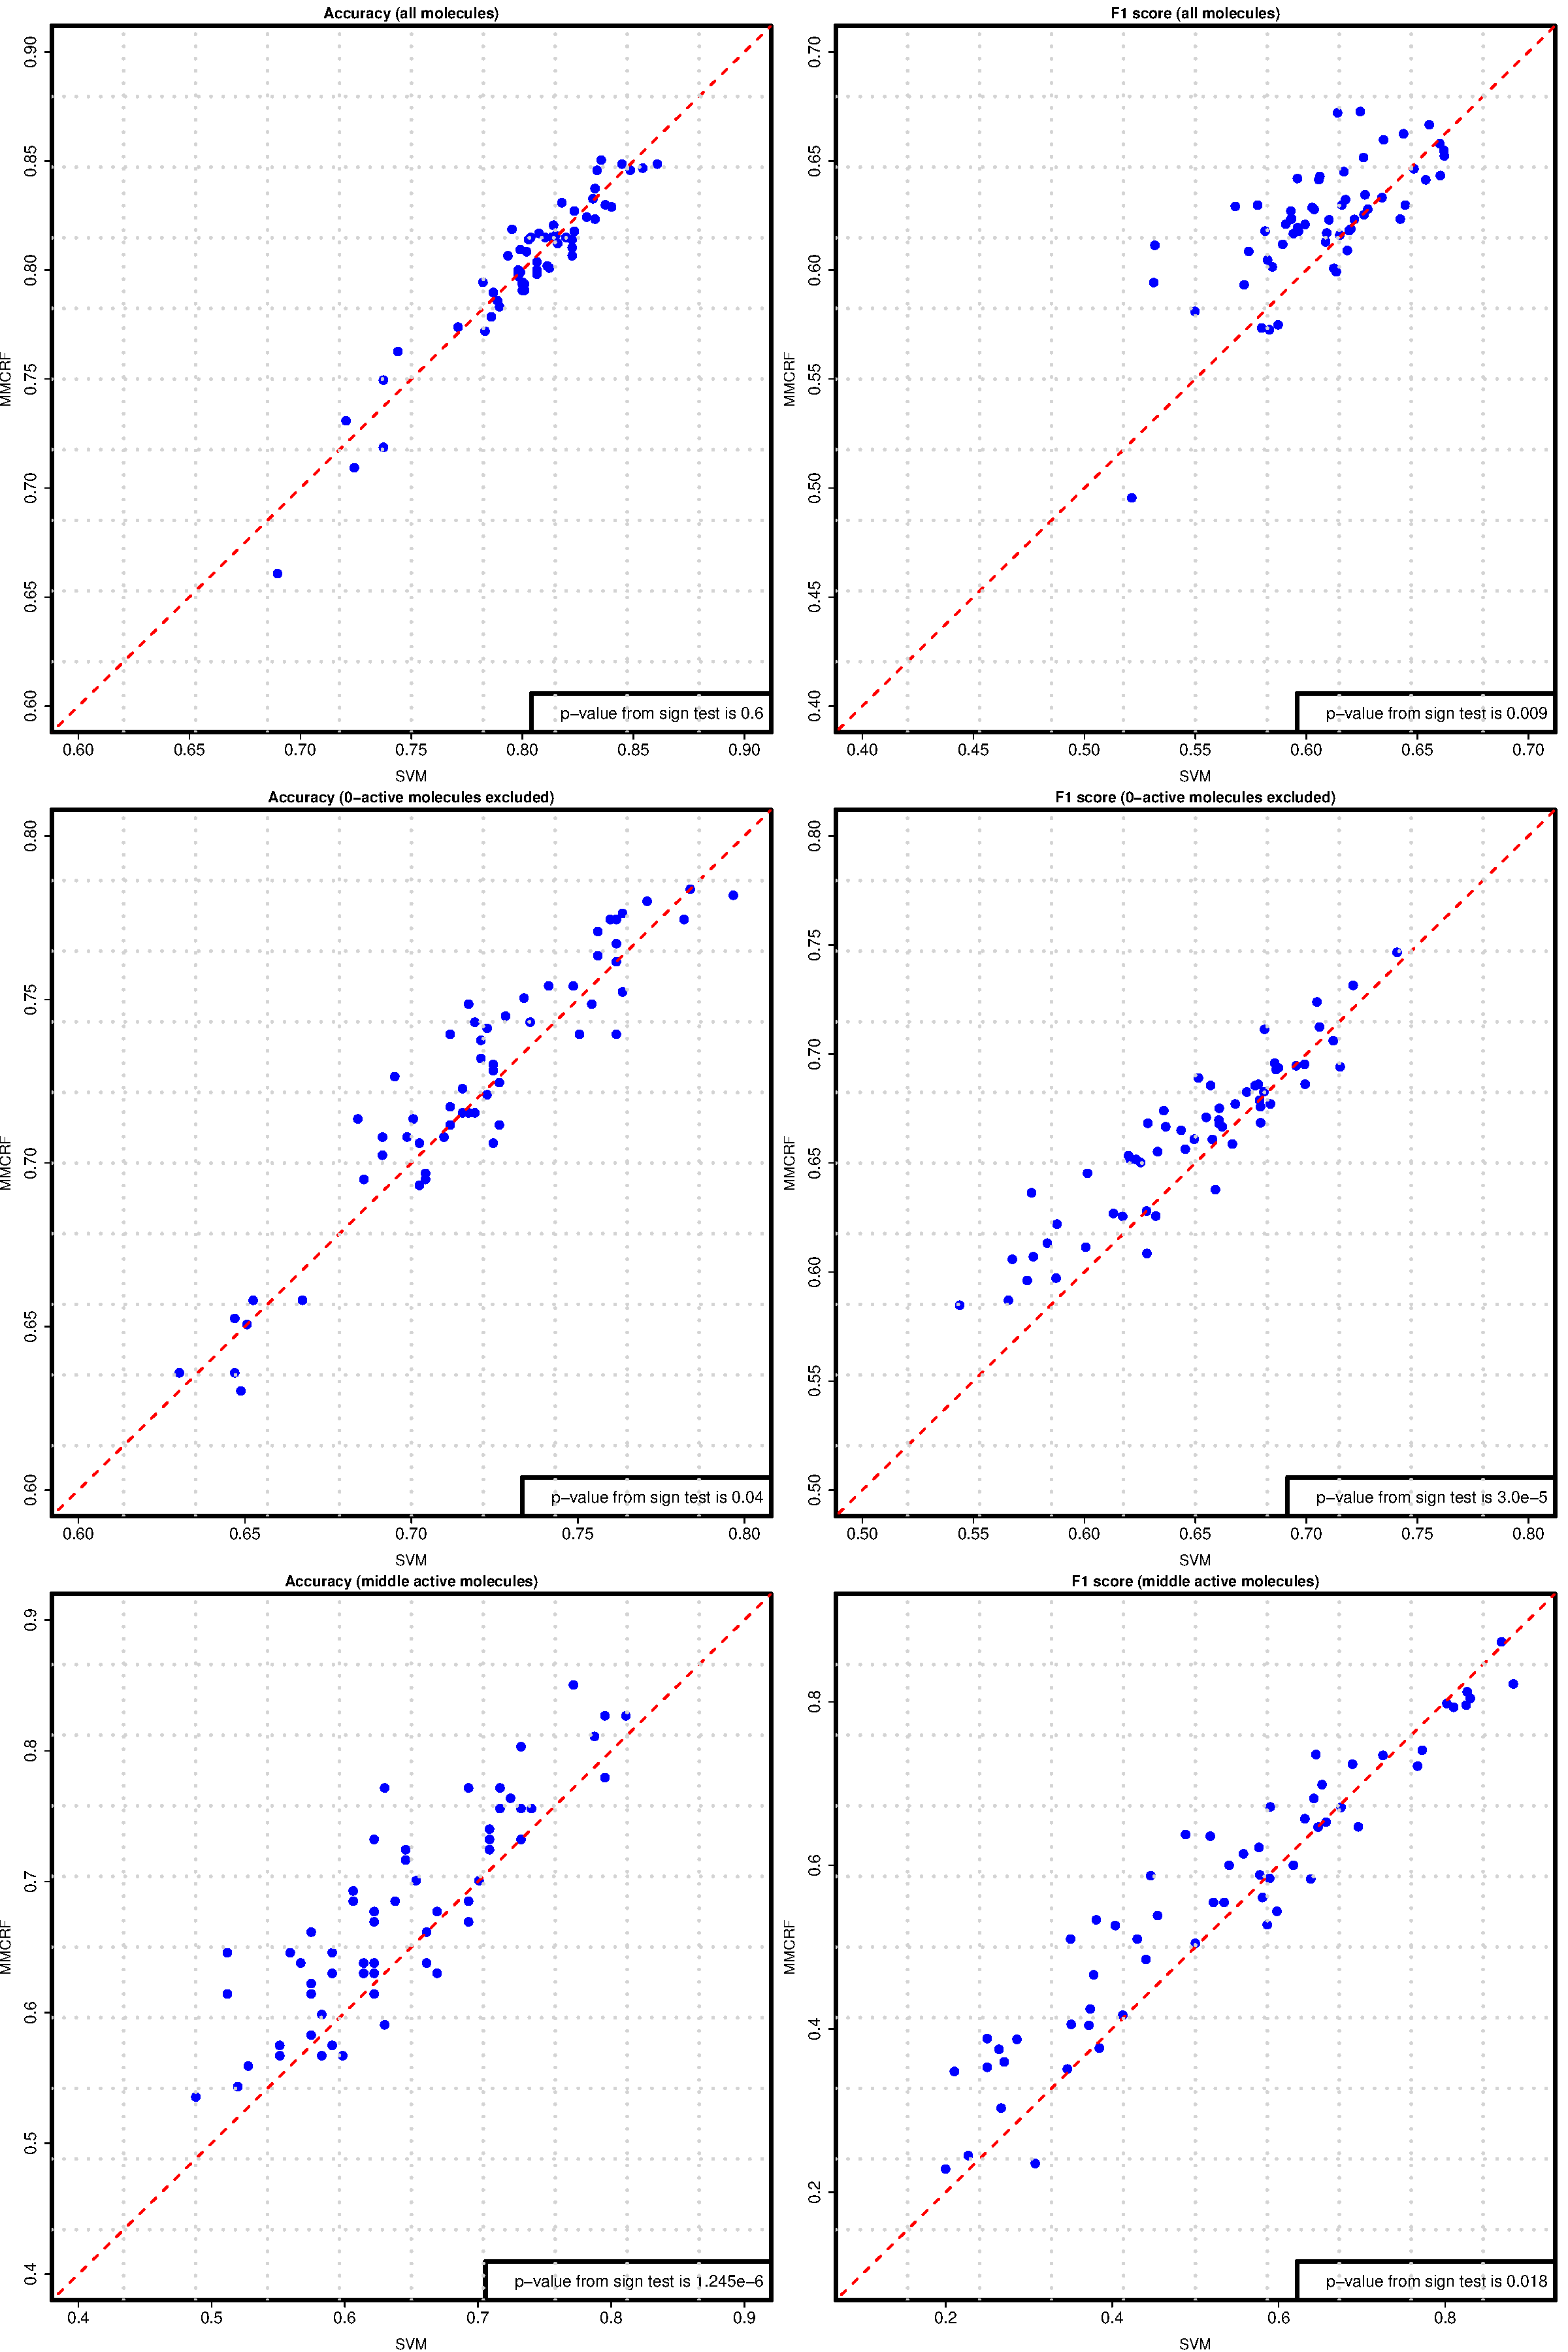
\includegraphics[width=1\columnwidth]{./plots/acc-f1-combined.pdf}
\caption[performance of MMCRF against SVM in cell lines.]{Scatter plot of accuracy (left) and F1 score (right) of MMCRF vs. SVM on Full data (top), No-Zero-Active  (middle) and Middle-Active molecules (bottom).}
\label{cellline_scatter_plot}
\end{figure}

\begin{figure}[p]
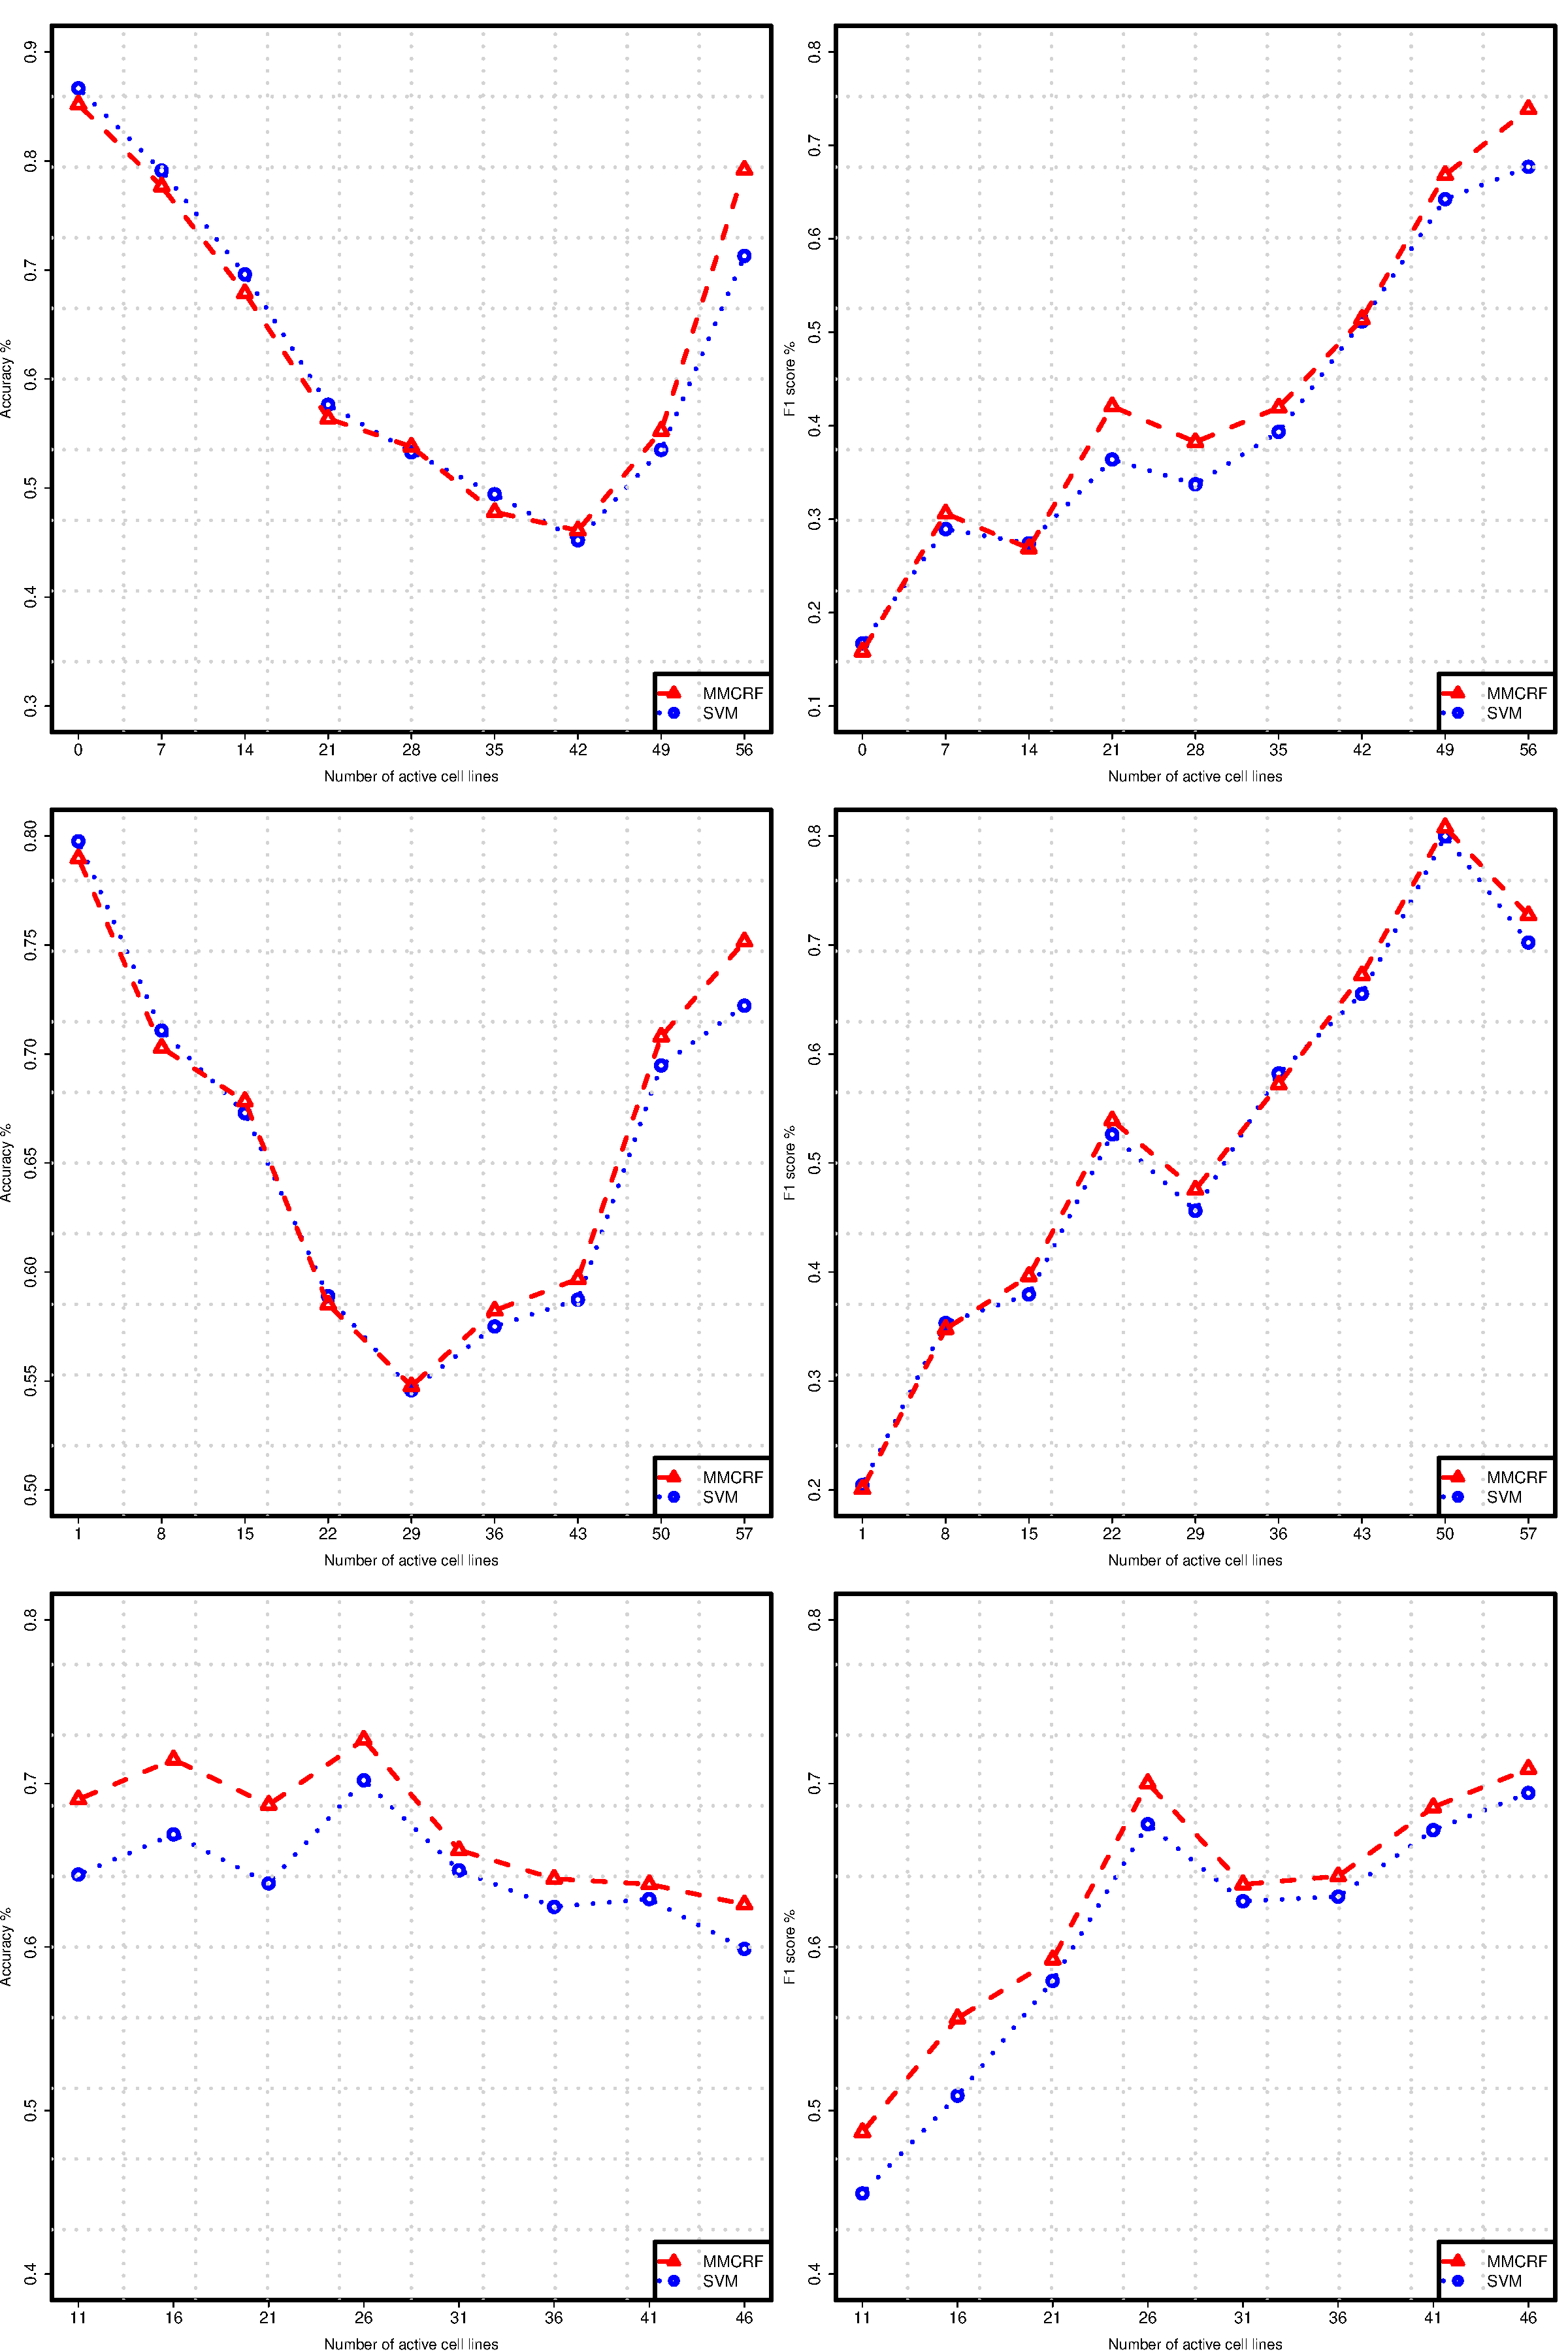
\includegraphics[width=1\columnwidth]{./plots/acc-f1-combined-cellline.pdf}
\caption[performance of MMCRF against SVM in active groups.]{Accuracy (left) and F1 score (right) of MMCRF vs. SVM on Full data (top), No-Zero-Active (middle) and Middle-Active molecules (bottom). Molecules are grouped according to their activities in the number of celllines, denoted as x-axis.}
\label{group_scatter_plot}
\end{figure}

We compare the performances of SVM and MMCRF classifiers in term of prediction accuracies and F1 scores on three versions of NCI-cancer dataset. We show overall accuracy and microlabel F1 score of MMCRF versus SVM for each cell line in Figure~\ref{cellline_scatter_plot}. Points above the diagonal line correspond to improvements in accuracies or F1 scores by MMCRF classifier. MMCRF improves the F1 score over SVM on each version of the data in statistically significant manner, as judged by the two-tailed sign test shown in Table~\ref{sign_test}. Accuracy is improved in two versions, No-Zero-Actives and the Middle-Active molecules, again in a statistically significant manner. Among the Middle-Active dataset, the difference in accuracy (bottom, left of Figure~\ref{cellline_scatter_plot}) is sometimes drastic, around 10 percentage units in favor of MMCRF for a significant fraction of the cell lines.


We categorize molecules into different groups according to their activities against the number of cell lines. We compare the accuracy and F1 score of MMCRF and SVM in each activity group on different versions of the dataset. The results\footnote{Average accuracies and F1 scores are calculated from each interval, shown as x-axis, in order to alleviate the random fluctuation.} are shown in Figure~\ref{group_scatter_plot}. In the first two versions of the dataset where biased molecular data exist, MMCRF classifier is always better than SVM classifier when the density of labels is high, which corresponds to the molecules that are active against many cell lines. They both made competitive predictions when the label density is low. While for the last version of dataset where biased molecules are removed, MMCRF classifier clearly outperforms SVM in all cases. The results further demonstrate that the predictions from SVM are highly affected by the biased molecules, the ones active against no cell lines or all cell lines.

\begin{center}
\begin{table}
\centering
\begin{tabular}{|c||c|c|}\hline
\multirow{2}{*}{\textbf{\em Dataset version}}
 & \multicolumn{2}{|c|}{\bf\em $p$-value from sign test} \\ \cline{2-3}
 & \textbf{\em Accuracy }  &\textbf{\em F1 score } \\ \hline \hline
Full & {0.6} & {0.009} \\ \hline
Non-Zero-Active & {0.04} & {3.0e-5} \\ \hline
Middle-Active& {1.2e-6} & {0.018} \\ \hline
\end{tabular}
\caption[Sign test.]{$p$-values from two tailed sign tests on different versions of NCI-cancer datasets. All $p$-values are statistically significant ($p\text{-value}<0.05$), except the one from accuracy comparison on full data.}
\label{sign_test}
\end{table}
\end{center}

\subsubsection{Agreements of predictions from SVM and MMCRF}


In molecular classification, positive predictions are more interesting than negative ones since they correspond to potential drug candidates. Therefore, we further check the positive and negative predictions from MMCRF and SVM on three versions of the datasets. Table~\ref{agreement_1} shows the results on dataset with full molecular data, Table~\ref{agreement_2} depicts the results by excluding zero-active molecules, and Table~\ref{agreement_3} illustrates the results by using only middle-active molecules. The results are calculated from the stratified 5-fold cross validation. Overall, MMCRF and SVM classifiers agree on most of positive and negative predictions (approximately $90\%$ and $95\%$ respectively). MMCRF is better at predicting positive labels, while SVM is better at negative ones. Since the original dataset is highly biased with $90\%$ of molecules being inactive against all cell lines, MMCRF is able to tackle this problem better than SVM.	

\begin{table}[t]\small
\begin{tabular}{|c||c|c||c|c|} \hline
 &  \multicolumn{2}{|c||}{\bf Positive class} &  \multicolumn{2}{|c|}{\bf Negative class}\\ \cline{2-5}
 	                       & SVM Correct & SVM Incorrect & SVM Correct & SVM Incorrect \\  \hline
MMCRF  Correct  & $48.6 \pm 4.1\%$ & $7.1 \pm 2.6\%$ & $88.0 \pm 4.9\%$ & $2.2 \pm 1.2\%$ \\ \hline
MMCRF Incorrect & $3.4 \pm 1.3\%$ & $40.9 \pm 3.4\%$ & $3.8 \pm 1.7\%$ &  $6.1 \pm 3.0\%$ \\ \hline
\end{tabular} 
\caption[Prediction agreements from MMCRF and SVM 1.]{Agreements of positive and negative predictions from both MMCRF and SVM on Full data.}
\label{agreement_1}
\end{table}

\begin{table}[t]\small
\begin{tabular}{|c||c|c||c|c|} \hline
 &  \multicolumn{2}{|c||}{\bf Positive class} &  \multicolumn{2}{|c|}{\bf Negative class}\\ \cline{2-5}
 	                       & SVM Correct & SVM Incorrect & SVM Correct & SVM Incorrect \\  \hline
MMCRF  Correct  & $57.9 \pm 5.7\%$ & $5.2 \pm 1.7\%$ & $74.4 \pm 10.5\%$ & $3.4 \pm 1.2\%$ \\ \hline
MMCRF Incorrect & $2.8 \pm 1.1\%$ & $34.1 \pm 5.3\%$ & $4.4 \pm 1.2\%$ &  $17.8 \pm 8.9\%$ \\ \hline
\end{tabular} 
\caption[Prediction agreements from MMCRF and SVM 2.]{Agreements of positive and negative predictions from both MMCRF and SVM on dataset without zero-active molecules.}
\label{agreement_2}
\end{table}

\begin{table}[t]\small
\begin{tabular}{|c||c|c||c|c|} \hline
 &  \multicolumn{2}{|c||}{\bf Positive class} &  \multicolumn{2}{|c|}{\bf Negative class}\\ \cline{2-5}
 	                       & SVM Correct & SVM Incorrect & SVM Correct & SVM Incorrect \\  \hline
MMCRF  Correct  & $41.5 \pm 25.9\%$ & $7.5 \pm 5.9\%$ & $57.7 \pm 26.6\%$ & $9.8 \pm 6.9\%$ \\ \hline
MMCRF Incorrect & $8.7 \pm 6.9\%$ & $42.3 \pm 25.1\%$ & $5.7 \pm 5.6\%$ &  $26.8 \pm 25.9\%$ \\ \hline
\end{tabular} 
\caption[Prediction agreements from MMCRF and SVM 3.]{Agreement of positive and negative predictions from both MMCRF and SVM on middle-active molecules.}
\label{agreement_3}
\end{table}




\subsubsection{Effect of loopy belief propagation}

We also tested different loopy belief propagation iteration parameters to see their effects on global optimization. In Figure~\ref{lbp_effect}, we report global objective values under different iteration parameters against time line. The best loopy belief propagation iteration parameter from the experiment was $11$, where objective value of MMCRF approached a global optimum in a short time. Smaller iteration parameter is not sufficient for MMCRF to reach a global optimum, while larger values incur convergence to need more time. The optimal loopy belief propagation iteration parameter turns out to be close to the diameter of the Markov network (10 in this case), indicating that propagation of messages through the network is required for best performance.

\begin{figure}
\begin{center}
\centering
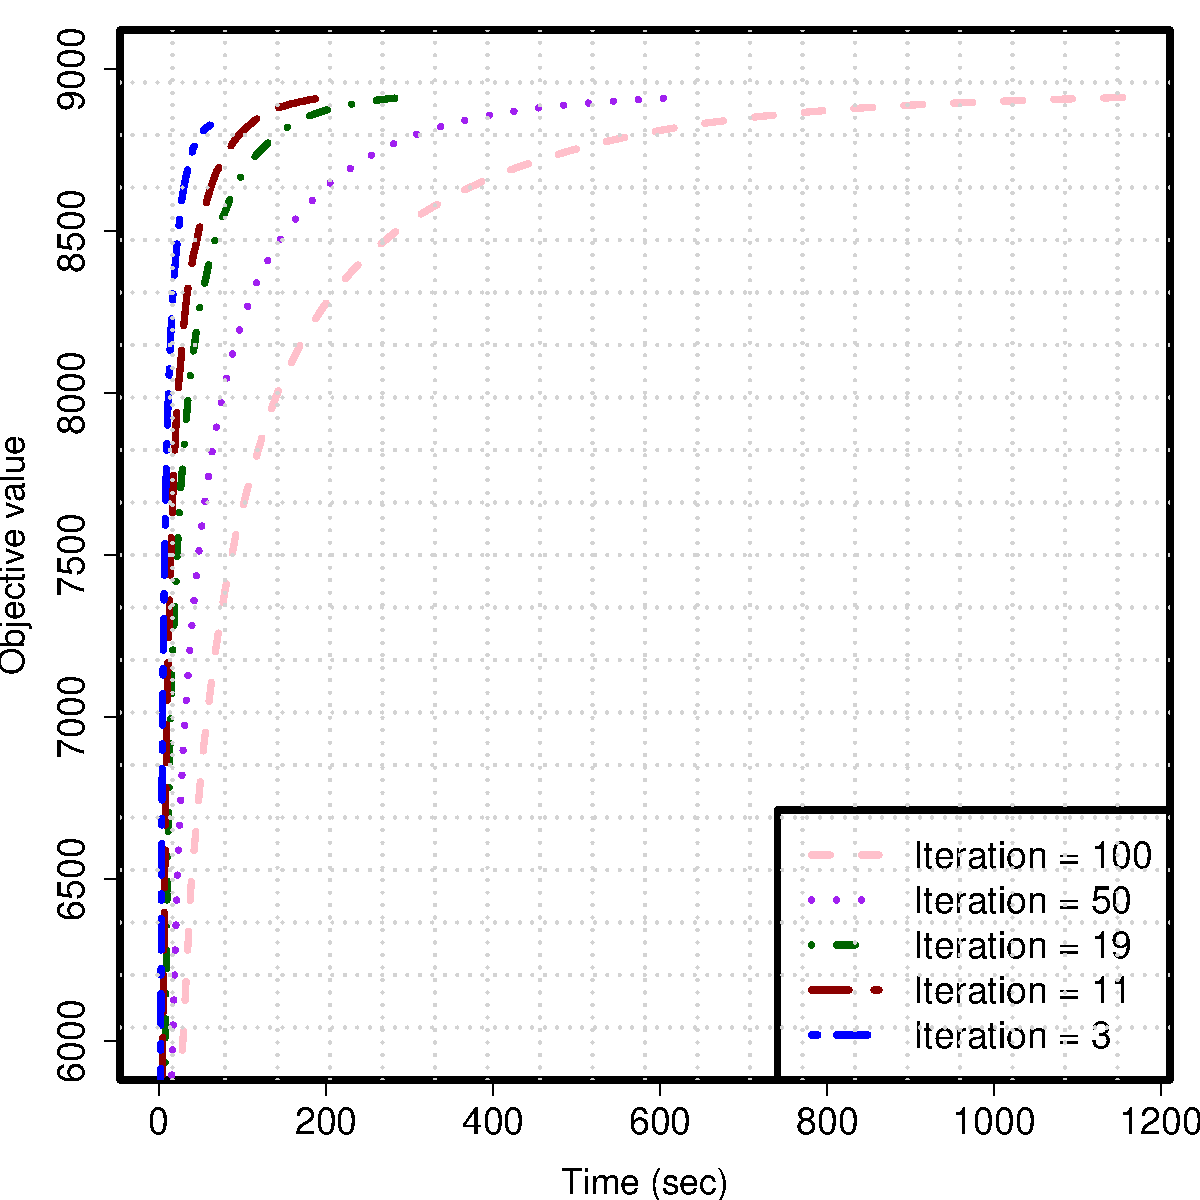
\includegraphics[width=0.6\columnwidth]{./plots/lbp_effect.pdf}
\caption[Effect of LBP parameter of MMCRF.]{Effect of loopy belief propagation iteration.}
\label{lbp_effect}
\end{center}
\end{figure}


\subsubsection{Computation time}

Besides predictive accuracy, training time of classifiers is important when a large number of drug targets need to be processed. The potential benefit of multilabel classification is the fact that only single model
needs to be trained instead of a bag of binary classifiers. We compared the running time needed to construct MMCRF classifier (implemented in native MATLAB) against libSVM classifier (C++). We conducted the experiment on a \(2.0\)GHz computer with \(8\)GB memory. Figure~\ref{cpu_time} shows that MMCRF scales better when training set increases.

\begin{figure}[t]
\begin{center}
\centering
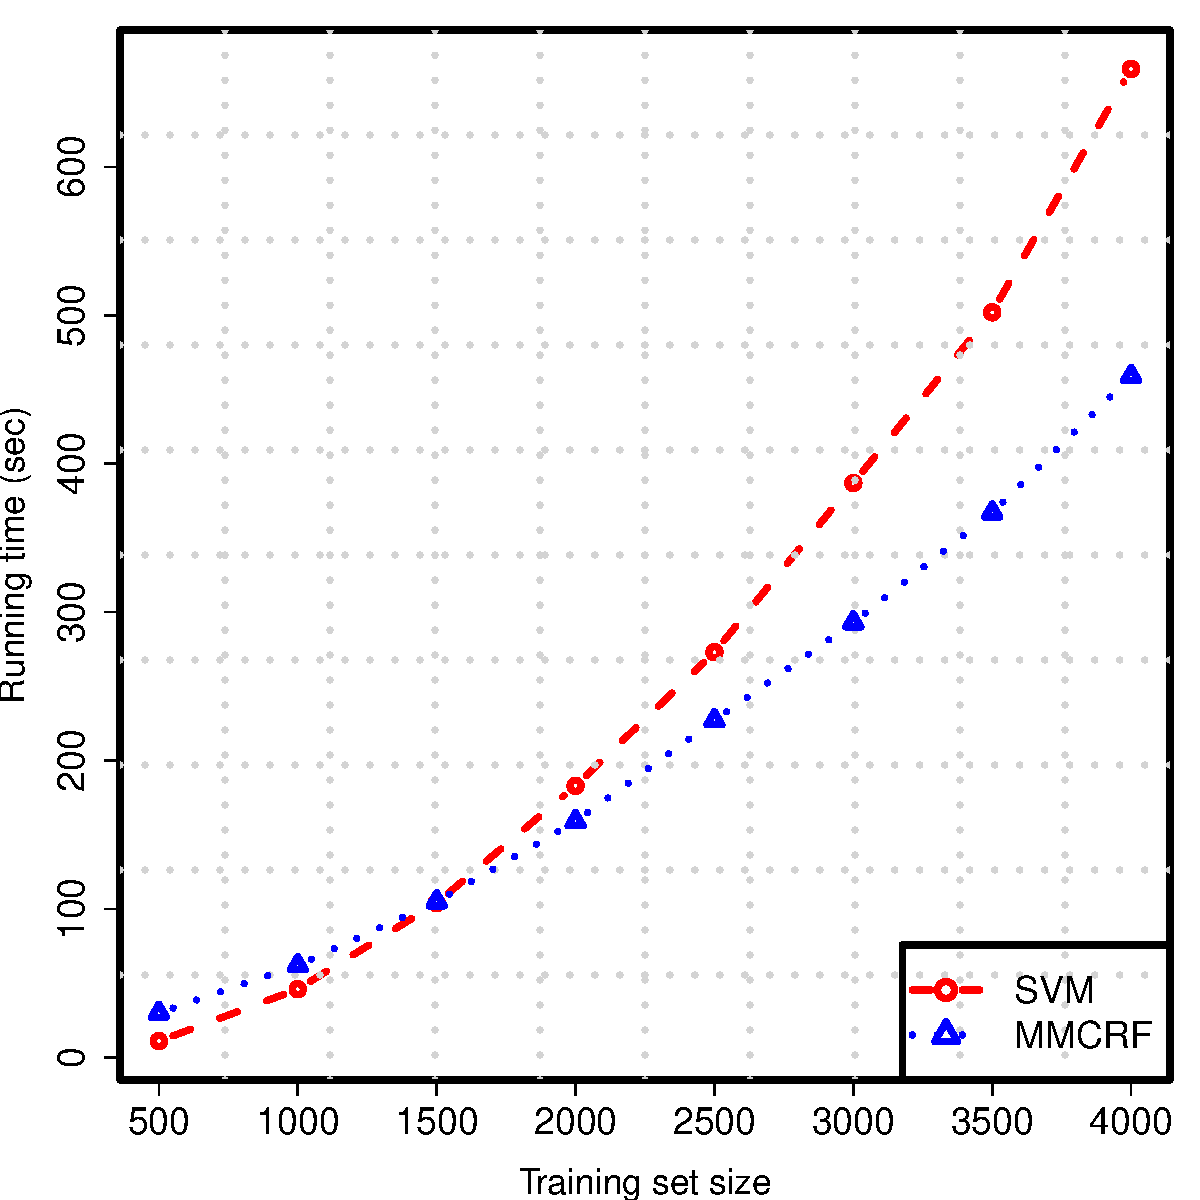
\includegraphics[width=0.6\columnwidth]{plots/cputime.pdf}
\caption[Training times from MMCRF against SVM.]{Training time for SVM and MMCRF classifiers on training sets of different sizes.}
\label{cpu_time}
\end{center}
\end{figure}



%%%%%%%%%%%%%%%%%%%%%%%%%%%%%%%%%%%%%%%%%%%%%%%%%%%%%%%%%%%%%%%%%%%%%%%%%%%%%%%%
%
% conclusion
%
%%%%%%%%%%%%%%%%%%%%%%%%%%%%%%%%%%%%%%%%%%%%%%%%%%%%%%%%%%%%%%%%%%%%%%%%%%%%%%%%
\clearpage
\section{Conclusions}

This work explores a machine learning approach for classification of drug-like molecules. Specifically, we focused on two learning algorithms and various graph kernel methods. Support vector machine (SVM) in binary classification scenario and max-margin conditional random field (MMCRF) tailored for multilabel classification task were addressed. We then reviewed and implemented several the state-of-the-art graph kernel methods, and evaluated their performances under binary classification setups. The best kernel method was selected, which achieved top accuracies on Mutag dataset and NCI-cancer dataset of different versions in our experiments.

The multilabel structural classification approach utilized by MMCRF algorithm assumes the dependencies between single labels and predicts all labels in one shot. Significant improvements over SVM classifiers on NCI-cancer dataset were achieved in our experiments by employing multilabel setups. Especially, MMCRF clearly outperformed SVM in one version of NCI-cancer dataset where biased molecules (the ones active against few cell lines or in many cell lines) were excluded.

The performance of MMCRF algorithm was also briefly described in the thesis. The experiment on loopy belief propagation shown that the inference algorithm converged when the iteration parameter was close to the diameter of the underlay network. Hence, the belief had time to propagate from one end of the network to another. The algorithm would not reach a global optimal with a small iteration parameter, and a large parameter only increased the converging time.

The Markov network for modeling the dependencies between the targets can be extracted from auxiliary data with different methods. Currently, only correlation thresholding was considered in our experiments. Other methods, for example graph lasso estimation, still remain mystery to us. Besides, reduced graph which maintains only important structures of original molecular graphs seems to be promising. We need more experiments to find out its effects on predictions. Furthermore, the necessity of the Markov network being generated from auxiliary data is another interesting direction. Comparative experiments are still needed for us to understand the differences between the meaningful networks and random ones. All these questions contribute to a good basis for future work. 



%%%%%%%%%%%%%%%%%%%%%%%%%%%%%%%%%%%%%%%%%%%%%%%%%%%%%%%%%%%%%%%%%%%%%%%%
%
% bibliography
%
%%%%%%%%%%%%%%%%%%%%%%%%%%%%%%%%%%%%%%%%%%%%%%%%%%%%%%%%%%%%%%%%%%%%%%%%
\clearpage
\nocite{*}
\bibliographystyle{tktl}
\bibliography{thesis}

\lastpage


%%%%%%%%%%%%%%%%%%%%%%%%%%%%%%%%%%%%%%%%%%%%%%%%%%%%%%%%%%%%%%%%%%%%%%%%
%
%	appendix
%
%%%%%%%%%%%%%%%%%%%%%%%%%%%%%%%%%%%%%%%%%%%%%%%%%%%%%%%%%%%%%%%%%%%%%%%%
\appendices



\end{document}

%%%%%%%%%%%%%%%%%%%%%%%%%%%%%%%%%%%%%%%%%%%%%%%%%%%%%%%%%%%%%%%%%%%%%%%%
%
%	END
%
%%%%%%%%%%%%%%%%%%%%%%%%%%%%%%%%%%%%%%%%%%%%%%%%%%%%%%%%%%%%%%%%%%%%%%%%
